% UCL Thesis LaTeX Template
% 
% This is a template/skeleton for PhD/MPhil/MRes theses.
%
% It uses a rather split-up file structure because this tends to
%  work well for large, complex documents.
% We suggest using one file per chapter, but you may wish to use more
%  or fewer separate files than that.
% We've also separated out various bits of configuration into their
%  own files, to keep everything neat.
% Note that the \input command just streams in whatever file you give
%  it, while the \include command adds a page break, and does some
%  extra organisation to make compilation faster. Note that you can't
%  use \include inside an \include-d file.
% We suggest using \input for settings and configuration files that
%  you always want to use, and \include for each section of content.
% If you do that, it also means you can use the \includeonly statement
%  to only compile up the section you're currently interested in.
% You might also want to put figures into their own files to be \input.

% For more information on \input and \include, see:
%  http://tex.stackexchange.com/questions/246/when-should-i-use-input-vs-include


% Formatting rules for theses are here: 
%  http://www.ucl.ac.uk/current-students/research_degrees/thesis_formatting
% Binding and submitting guidelines are here:
%  http://www.ucl.ac.uk/current-students/research_degrees/thesis_binding_submission

% This package goes first and foremost, because it checks all 
%  your syntax for mistakes and some old-fashioned LaTeX commands.
% Note that normally you should load your documentclass before 
%  packages, because some packages change behaviour based on
%  your document settings.
% Also, for those confused by the RequirePackage here vs usepackage
%  elsewhere, usepackage cannot be used before the documentclass
%  command, while RequirePackage can. That's the only functional
%  difference.
\RequirePackage[l2tabu, orthodox]{nag}


% ------ Main document class specification ------
% The draft option here prevents images being inserted,
%  and adds chunky black bars to boxes that are exceeding 
%  the page width (to show that they are).
% The oneside option can optionally be replaced by twoside if
%  you intend to print double-sided. Note that this is
%  *specifically permitted* by the UCL thesis formatting
%  guidelines.
%
% Valid options in terms of type are:
%  phd
%  mres
%  mphil
%\documentclass[12pt,phd,draft,a4paper,oneside]{ucl_thesis}
\documentclass[12pt,phd,a4paper,oneside]{ucl_thesis}


% Package configuration:
%  LaTeX uses "packages" to add extra commands and features.
%  There are quite a few useful ones, so we've put them in a 
%   separate file.
% -------- Packages --------

% This package just gives you a quick way to dump in some sample text.
% You can remove it -- it's just here for the examples.
\usepackage{blindtext}

% This package means empty pages (pages with no text) won't get stuff
%  like chapter names at the top of the page. It's mostly cosmetic.
\usepackage{emptypage}

% The graphicx package adds the \includegraphics command,
%  which is your basic command for adding a picture.
\usepackage{graphicx}

% This command is provided by the graphicx package, and 
%  controls the default dpi resolution of images you use.
%  72 is the default, but 300 is more normal, and 600 is
%  as good as you can expect to be able to get on normal paper.
\pdfimageresolution=300


% The float package improves LaTeX's handling of floats,
%  and also adds the option to *force* LaTeX to put the float
%  HERE, with the [H] option to the float environment.
\usepackage{float}

% The amsmath package enhances the various ways of including
%  maths, including adding the align environment for aligned
%  equations.
\usepackage{amsmath}

% Use these two packages together -- they define symbols
%  for e.g. units that you can use in both text and math mode.
\usepackage{gensymb}
\usepackage{textcomp}
% You may also want the units package for making little
%  fractions for unit specifications.
%\usepackage{units}


% The setspace package lets you use 1.5-sized or double line spacing.
\usepackage{setspace}
\setstretch{1.5}

% That just does body text -- if you want to expand *everything*,
%  including footnotes and tables, use this instead:
%\renewcommand{\baselinestretch}{1.5}


% PGFPlots is either a really clunky or really good way to add graphs
%  into your document, depending on your point of view.
% There's waaaaay too much information on using this to cover here,
%  so, you might want to start here:
%   http://pgfplots.sourceforge.net/
%  or here:
%   http://pgfplots.sourceforge.net/pgfplots.pdf
%\usepackage{pgfplots}
%\pgfplotsset{compat=1.3} % <- this fixed axis labels in the version I was using

% PGFPlotsTable can help you make tables a little more easily than
%  usual in LaTeX.
% If you're going to have to paste data in a lot, I'd suggest using it.
%  You might want to start with the manual, here:
%  http://pgfplots.sourceforge.net/pgfplotstable.pdf
%\usepackage{pgfplotstable}

% These settings are also recommended for using with pgfplotstable.
%\pgfplotstableset{
%	% these columns/<colname>/.style={<options>} things define a style
%	% which applies to <colname> only.
%	empty cells with={--}, % replace empty cells with '--'
%	every head row/.style={before row=\toprule,after row=\midrule},
%	every last row/.style={after row=\bottomrule}
%}


% The mhchem package provides chemistry formula typesetting commands
%  e.g. \ce{H2O}
%\usepackage[version=3]{mhchem}

% And the chemfig package gives a weird command for adding Lewis 
%  diagrams, for e.g. organic molecules
%\usepackage{chemfig}

% The linenumbers command from the lineno package adds line numbers
%  alongside your text that can be useful for discussing edits 
%  in drafts.
% Remove or comment out the command for proper versions.
%\usepackage[modulo]{lineno}
% \linenumbers 


% Alternatively, you can use the ifdraft package to let you add
%  commands that will only be used in draft versions
%\usepackage{ifdraft}

% For example, the following adds a watermark if the draft mode is on.
%\ifdraft{
%  \usepackage{draftwatermark}
%  \SetWatermarkText{\shortstack{\textsc{Draft Mode}\\ \strut \\ \strut \\ \strut}}
%  \SetWatermarkScale{0.5}
%  \SetWatermarkAngle{90}
%}


% The multirow package adds the option to make cells span 
%  rows in tables.
\usepackage{multirow}


% Subfig allows you to create figures within figures, to, for example,
%  make a single figure with 4 individually labeled and referenceable
%  sub-figures.
% It's quite fiddly to use, so check the documentation.
%\usepackage{subfig}

% The natbib package allows book-type citations commonly used in
%  longer works, and less commonly in science articles (IME).
% e.g. (Saucer et al., 1993) rather than [1]
% More details are here: http://merkel.zoneo.net/Latex/natbib.php
%\usepackage{natbib}

% The bibentry package (along with the \nobibliography* command)
%  allows putting full reference lines inline.
%  See: 
%   http://tex.stackexchange.com/questions/2905/how-can-i-list-references-from-bibtex-file-in-line-with-commentary
\usepackage{bibentry} 

% The isorot package allows you to put things sideways 
%  (or indeed, at any angle) on a page.
% This can be useful for wide graphs or other figures.
%\usepackage{isorot}

% The caption package adds more options for caption formatting.
% This set-up makes hanging labels, makes the caption text smaller
%  than the body text, and makes the label bold.
% Highly recommended.
\usepackage[format=hang,font=small,labelfont=bf]{caption}

% If you're getting into defining your own commands, you might want
%  to check out the etoolbox package -- it defines a few commands
%  that can make it easier to make commands robust.
\usepackage{etoolbox}


% IRINA's Packages
\usepackage[normalem]{ulem}
\usepackage{caption}
\usepackage{subcaption}

% Sets up links within your document, for e.g. contents page entries
%  and references, and also PDF metadata.
% You should edit this!
%%
%% This file uses the hyperref package to make your thesis have metadata embedded in the PDF, 
%%  and also adds links to be able to click on references and contents page entries to go to 
%%  the pages.
%%

% Some hacks are necessary to make bibentry and hyperref play nicely.
% See: http://tex.stackexchange.com/questions/65348/clash-between-bibentry-and-hyperref-with-bibstyle-elsart-harv
\usepackage{bibentry}
\makeatletter\let\saved@bibitem\@bibitem\makeatother
\usepackage[pdftex,hidelinks]{hyperref}
\makeatletter\let\@bibitem\saved@bibitem\makeatother
\makeatletter
\AtBeginDocument{
    \hypersetup{
        pdfsubject={Thesis Subject},
        pdfkeywords={Thesis Keywords},
        pdfauthor={Author},
        pdftitle={Title},
    }
}
\makeatother
    


% And then some settings in separate files.
% These settings are from:
%  http://mintaka.sdsu.edu/GF/bibliog/latex/floats.html

% They give LaTeX more options on where to put your figures, and may
%  mean that fewer of your figures end up at the tops of pages far
%  away from the thing they're related to.

% Alters some LaTeX defaults for better treatment of figures:
% See p.105 of "TeX Unbound" for suggested values.
% See pp. 199-200 of Lamport's "LaTeX" book for details.

%   General parameters, for ALL pages:
\renewcommand{\topfraction}{0.9}	% max fraction of floats at top
\renewcommand{\bottomfraction}{0.8}	% max fraction of floats at bottom

%   Parameters for TEXT pages (not float pages):
\setcounter{topnumber}{2}
\setcounter{bottomnumber}{2}
\setcounter{totalnumber}{4}     % 2 may work better
\setcounter{dbltopnumber}{2}    % for 2-column pages
\renewcommand{\dbltopfraction}{0.9}	% fit big float above 2-col. text
\renewcommand{\textfraction}{0.07}	% allow minimal text w. figs

%   Parameters for FLOAT pages (not text pages):
\renewcommand{\floatpagefraction}{0.7}	% require fuller float pages
% N.B.: floatpagefraction MUST be less than topfraction !!
\renewcommand{\dblfloatpagefraction}{0.7}	% require fuller float pages

% remember to use [htp] or [htpb] for placement,
% e.g. 
%  \begin{figure}[htp]
%   ...
%  \end{figure} % For things like figures and tables
\bibliographystyle{unsrt}   % For bibliographies

% Title Settings
\setcounter{secnumdepth}{3}
\setcounter{tocdepth}{3}
\title{Enhancing POSSUM with Parallel Imaging Capabilities}
\author{Irina Grigorescu}
\department{Microstructure Imaging Group \\ Centre for Medical Image Computing}


\begin{document}



\nobibliography*
% This is a dumb trick that works with the bibentry package to let
%  you put bibliography entries whereever you like.
% I used this to put references to papers a chapter's work was 
%  published in at the end of that chapter.
% For more information, see: http://stefaanlippens.net/bibentry

% If you haven't finished making your full BibTex file yet, you
%  might find this useful -- it'll just replace all your
%  citations with little superscript notes.
% Uncomment to use.
%\renewcommand{\cite}[1]{\emph{\textsuperscript{[#1]}}}

% At last, content! Remember filenames are case-sensitive and 
%  *must not* include spaces.
\maketitle
\makedeclaration

\begin{abstract} % 300 word limit
Magnetic Resonance Imaging (MRI) is an imaging technique which is widely used clinically as it is non-invasive and uses non-ionising radiation. However, MRI has a few potential drawbacks which include motion artifacts caused by patient movement and the high costs involved with every scan. In order to mitigate these problems, a collection of acquisition and reconstruction algorithms called parallel imaging techniques (pMRI) are clinically used in conjunction with already established MRI sequences in order to reduce scan time. However, as with any other MRI techniques, these are also prone to a handful of problems which need to be investigated in a controlled and reliable manner. The  only  way  of  accurately  assessing  the  reconstruction schemes which are used in pMRI is to simulate the parallel imaging acquisition pipeline.  As a result, the main aim of this thesis is to enhance an already existing MRI simulator called POSSUM with parallel imaging capabilities and to evaluate a popular image based reconstruction algorithm called SENSE under various combinations of parameters. For this, three objectives were met. First, multi-coil capabilities were added to POSSUM. This is an important first step as pMRI techniques rely on the sensitivity profiles of the phased-array receiver coils. Second, a parallel imaging pipeline was simulated with the enhanced version of POSSUM. Using  the  newly  enhanced  POSSUM, simulations of  increasing  acceleration  factors  were  performed for multiple types of coil geometries and sensitivity profiles. Finally, the quality of SENSE reconstructions and its robustness to noise was evaluated for various acceleration factors. The work has the potential to be extended and integrated seamlessly into the proposed simulator environment. %Moreover, it can be paired with diffusion MRI simulations to more accurately represent underlying brain microstructure.





\end{abstract}

\begin{acknowledgements}
First of all I would like to thank my supervisor Dr. Gary Hui Zhang for his constant support, invaluable guidance and all of our debugging and problem solving sessions. I would also like to thank Dr. Ivana Drobnjak for all the hours she spent explaining MR simulation concepts and for her constant moral support. Special thanks goes to my colleague and friend, Danny Raj Ramasawmy, for all those times he helped me disentangle a problem. I would also like to thank my fiance, Tudor, for being there for me every time I needed him to be. Finally, I would like to thank both my families, the one back home and the one I found here within the CDT group. 
\end{acknowledgements}

\setcounter{tocdepth}{2} 
% Setting this higher means you get contents entries for
%  more minor section headers.

\tableofcontents
\listoffigures
\listoftables


\chapter{Introduction}
\label{chapterlabel1}

%%%%%%%%%%%%%%%%%%%%%%%%%%
\section{Motivation}

Magnetic Resonance Imaging is an imaging technique that is widely used today in clinics and medical  research facilities to aid the understanding of how the human body works. It has many applications in the biomedical sciences such as the study of human anatomy, pathology and even function. Clinically, magnetic resonance imaging is also commonly preferred over other imaging modalities as it can provide good soft tissue contrast, it is non-invasive and uses non-ionising radiation.

However, MRI has a few potential drawbacks. First of all, MRI scans are expensive due to the high costs involved in purchasing and maintaining an MRI scanner. As the cost per scan is generally proportional to the scanning time, a large body of research is being done in trying to reduce the amount of time needed for a scan. Secondly, the imaging process is sensitive to movement. Any type of motion, such as patient motion, pulsatile flow, and even external disturbances, can affect the quality of the resulting MRI images. Hence, there is a need to mitigate these problems. One way to do so is to use parallel imaging techniques. 

Partially parallel magnetic resonance imaging is a class of acquisition schemes and reconstruction algorithms that uses less time to produce the same images as with a standard MRI pipeline. The advantage of pMRI is that it can be used in conjunction with well established MRI sequences. In fact, pMRI has become a standard in many clinically available scanners, as it can reduce scanning time as much as 2 or even 3 times the original without losing spatial resolution. However, as with all other MRI techniques, these are also prone to a handful of problems which need to be investigated in a controlled and reliable manner. 

Given that the only way to accurately assess the reconstruction algorithms used in pMRI techniques is to use an MRI simulator, the aim of this thesis is to accurately simulate the entire parallel imaging pipeline. In order to accomplish this, an existing MRI simulator, called POSSUM (\textit{Physics Oriented Simulated Scanner for Understanding MRI}), was used. This decision was influenced by both the open source nature of the simulator and its lack of support for multiple channel acquisitions. As a result, this project was focused on enhancing POSSUM with parallel imaging capabilities.

%%%%%%%%%%%%%%%%%%%%%%%%%%
\section{Scope and Objectives}

The aims of the research presented in this thesis are to build upon the structure of an already available  MRI simulator called POSSUM and to test the quality of reconstructions performed with an image-based reconstruction algorithm under various circumstances. In order to achieve this, the following objectives are to be met:

\begin{itemize}
    \item \textit{Enhance POSSUM with multi-coil acquisition}. The first step towards the parallel imaging pipeline is to make multi-coil acquisition possible within POSSUM. For this, arrays of multi-channel RF receiver coils of different sensitivity profiles were generated and used in our simulations. 
    
    \item \textit{Simulate parallel imaging with enhanced POSSUM}. Using the newly enhanced POSSUM, simulations of increasing acceleration factors were performed for multiple types of coil geometries and sensitivity profiles.
    %In pMRI techniques, an array of non-homogeneous receiver coils is used to collect the signal during readout. Each of these channels will have an associated sensitivity profile which describes how sensitive the respective coil is to the signal originating from a certain spatial location within the object. As the sensitivity profiles were generated previously, the next step is to use them in the simulation pipeline for a variety of parameter combinations. These parameters are: the number of channels in the array, the spatial variation of the coil sensitivity profile, the pMRI acceleration factor and the level of noise added to the sensitivity maps of the coils.
    
    \item \textit{Evaluate the performance of SENSE-type reconstructions}. An image-based reconstruction algorithm was used in conjunction with the dataset generated previously to evaluate the quality of reconstruction and the robustness to noise of the proposed SENSE algorithm.
    
    % \begin{itemize}
    %     \item \textit{The number of channels in the array}. This parameters will be varied starting from a 2-channel array up to a 16-channel array.
    
    %     \item \textit{The spatial variation of the coil sensitivity profile}. This parameter describes how much of the field-of-view is covered and how sensitive a specific coil is to the signal generating from a spatial location within the object.
    
    %     \item \textit{The acceleration factor $R$}. This parameter describes the amount of scanning time reduction. 
        
    %     \item \textit{The amount of noise added to the sensitivity profiles of the coils}.
    % \end{itemize}
    
    % \item Every non-homogeneous coil in the array must be able to acquire undersampled k-space data in the phase-encoding direction. 
    %     %As a result, the reconstructed field-of-view will be smaller than the object being imaged, leading to aliasing artifacts in the phase-encoding direction of the final images.
        
    
    % \item \textit{Use POSSUM to create aliased images by reducing the scanning time}. Aliasing occurs when the k-space is undersampled, leading to a smaller reconstructed field-of-view than the object being imaged. By reducing the phase-encoding steps of, for example an EPI sequence acquisition, aliasing will occur in the final images in the phase-encoding direction.
    
    % \item \textit{Perform image-based parallel imaging reconstructions (more specifically, the SENSE reconstruction algorithm) for different acceleration factors}. A SENSE-based reconstruction algorithm was tested with the POSSUM generated aliased images and the coil sensitivity maps for various acceleration factors $R = \{1, 2, 3, 4\}$.
    
    % \item \textit{Investigate the effect of noise on SENSE reconstructions}. Noise is inherently present in all MRI scans and is also a big issue in parallel imaging techniques. For this, the effect of noise added to coil sensitivity profiles was investigated.
    
    % \item \textit{Investigate whether motion can be averted when scanning time is reduced}. Motion is supposedly the most frequent source of artifacts in MRI images. Parallel imaging techniques are known to solve this issue by lowering the scanning time and thus reducing the probability of motion happening during acquisition. For this, a proof of concept experiment was devised to show that higher acceleration factors will be less prone to motion. 
    
\end{itemize}

%%%%%%%%%%%%%%%%%%%%%%%%%%
\section{Thesis Outline}

This project aims to develop a parallel imaging pipeline within the state-of-the-art simulator called POSSUM. In accomplishing this, a certain path mush be taken. 

First, a good understanding of the MRI physics must be shown. For this, \textbf{Chapter 2 (Magnetic Resonance Imaging)} describes the building blocks for understanding the physical concepts of the MRI pipeline and, therefore, the more advanced techniques described later on. This chapter will take the reader from the physical concepts of nuclear magnetic resonance, to the steps required for MR image formation and, finally, the motivation for and the important concepts of parallel imaging techniques.

Second, as simulation is the key player in this research, \textbf{Chapter 3 (MRI Simulation)} sets the scene for currently active MRI simulators. The main aim of this chapter is to place POSSUM (the simulator used throughout this thesis) into the MRI simulation context and to identify the most sought for simulator features.

Third, an in-depth description of how the pipeline was implemented is provided in \textbf{Chapter 4 (Simulating Parallel Imaging)}. More specifically, this chapter describes the methods used for simulating parallel imaging within POSSUM and it is also equipped with a comprehensive description of the reconstruction algorithm used for all our experiments.

Next, we demonstrate that the proposed pipeline is viable. Namely, multiple receiver surface coil acquisition is shown to work within POSSUM and parallel imaging is simulated under different combinations of parameters. These results are to be found in \textbf{Chapter 5 (Results)}.

The final remarks, together with the conclusions and future work will be outlined in \textbf{Chapter 6 (Conclusions and Future Work)}. This chapter ties everything together by presenting, on top of current limitations of the work and future improvements, the long term aim of my PhD thesis.


\chapter{Magnetic Resonance Imaging}
\label{chapterlabel2}

This section provides the necessary mathematical background for understanding the magnetic resonance imaging process. It starts with describing the NMR (nuclear magnetic resonance) phenomena which are at the heart of magnetic resonance imaging, continues with the basic concepts behind image formation and ends with a description of parallel imaging, the main focus of this thesis.

%%%%%%%%%%%%%%%%%%%%%%%%%%
\section{NMR Physics}
Magnetic resonance imaging (MRI) is a non-invasive imaging technique that is based on the physical phenomena of atomic nuclei (protons) responding and interacting with external magnetic fields. The key participant in the process of constructing MR images is the hydrogen proton, the most abundant element in our bodies. In fact, other species of protons can also be used, but in this thesis the main focus is on the hydrogen proton. For the most part, an MRI experiment is made up of two steps. First, a series of magnetic fields are used to manipulate the proton 'spin' orientation in order to create a net magnetization arising from the collective spins. Second, this net magnetization is manipulated with radio frequency magnetic fields in order to be measured using a coil detector. That being said, in this subsection the focus is on the underlying physics of magnetic resonance imaging, starting from the behaviour of a single magnetic moment placed in a static magnetic field and ending with the principles of signal detection.

%%%%%%%%%%%%%
\subsection{Classical Response of a Single Nucleus to a Magnetic Field}
In magnetic resonance imaging the key participator is the magnetic moment of the proton. In this subsection the fundamental interaction of a proton when placed in a static magnetic field is described.

Following the work of Stern and Gerlach in the early 1920's, 
a fundamental property of an odd numbered atomic nucleus was inferred from experiment. 
This property is called \textit{angular momentum $\vec{J}$} (or \textit{spin}) and it gives rise, from a classical perspective, to a small \textit{magnetic moment} $\vec{\mu}$. 
The relationship between the two properties is found from experiment:

\begin{equation} \label{eq:21}
    \vec{\mu} = \gamma \vec{J}
\end{equation}

where $\gamma$ is called the \textit{gyromagnetic ratio} and it is a particle dependent constant. For hydrogen nuclei, this quantity is found to be:

\begin{equation} \label{eq:22}
    \gamma_{H} = 2.675 \times 10^8 \text{  } rad/s/T
\end{equation}

or the 'gamma-bar' quantity:

\begin{equation} \label{eq:23}
    \text{\sout{$\gamma$}}_H \equiv \frac{\gamma}{2 \pi} = 42.58 \text{  } MHz/T
\end{equation}
where T is Tesla, the unit for magnetic field strength, and it is the equivalent of $10,000$ Gauss \cite{Haacke1999}.

In addition, when placing the spin in an external magnetic field $\vec{B}$, it will experience a torque $\vec{N}$ that will align the magnetic moment $\vec{\mu}$ along the direction of the field according to
\begin{equation} \label{eq:24}
    \vec{N} = \vec{\mu} \times \vec{B}
\end{equation}
Furthermore, knowing that a nonzero net torque on a loop implies that the total angular momentum $\vec{J}$ will change with:

\begin{equation} \label{eq:25}
    \frac{d\vec{J}}{dt} = \vec{N}
\end{equation}

and taking into account equations \ref{eq:21} and \ref{eq:24}, we find the following:

\begin{equation} \label{eq:26}
    \frac{d\vec{\mu}}{dt} = \gamma \vec{\mu} \times \vec{B}
\end{equation}
which is the fundamental equation of motion for a single spin in a magnetic field.

Furthermore, by forming a scalar (dot) product of both sides of equation \ref{eq:26} we get:

\begin{flalign*}
	\frac{d\vec{\mu}}{dt} \cdot \vec{\mu} + \vec{\mu} \cdot
	     \frac{d\vec{\mu}}{dt} &= 0  \Rightarrow \\
	\frac{d(\vec{\mu} \cdot \vec{\mu})}{dt} &= 0  \Rightarrow \\
	\frac{d\mu^2}{dt} &= 0 \Rightarrow \\
	\frac{d \mu}{dt} \, \mu + \mu \, \frac{d \mu}{dt} &= 0 \Rightarrow \\
	2 \, \mu \, \frac{d \mu}{dt} &= 0 \Rightarrow \\
	\frac{d \mu}{dt} &= 0
\end{flalign*}

which shows that the magnitude of the magnetic moment does not change with time. On the other hand, the direction of the magnetic moment does change with time, the cross product between $\vec{\mu}$ and $\vec{B}$ 'pushing' the tip of the magnetic moment vector in a clockwise precession. This behaviour is shown in Figure~\ref{fig:21} where the angular frequency of precession is found with the following deduction: \\

We know that:
\begin{equation} \label{eq:27}
    \lvert d\vec{\mu} \rvert = 
        \lvert \vec{\mu} \rvert sin \theta \lvert d \phi \rvert 
\end{equation}

But we also know that:
\begin{equation} \label{eq:28}
    \lvert d\vec{\mu} \rvert = 
        \gamma \lvert \vec{\mu} \times \vec{B} \rvert dt = 
        \gamma \, \mu \, B \, sin \theta \, dt 
\end{equation}

Therefore, from equations \ref{eq:27} and \ref{eq:28} above we get:
\begin{equation} \label{eq:29}
    \lvert d\phi \rvert = \gamma \, B \, \lvert dt \rvert
\end{equation}

which brings us to the well-known \textit{Larmor precession} formula given below:
\begin{equation} \label{eq:210}
    \omega \equiv \lvert \frac{d\phi}{dt} \rvert = \gamma B
\end{equation}

This equation is at the heart of MR imaging as it relates the strength of the magnetic field and the frequency of the spins' precession. 

\begin{figure}[ht]
    \centering
    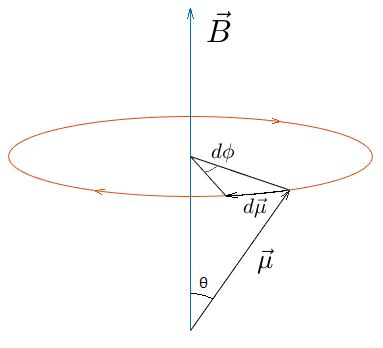
\includegraphics[width=0.7\textwidth,keepaspectratio]{precession}
    \caption{Clockwise precession of a proton's spin about a magnetic field}
    \label{fig:21}
\end{figure}

%%%%%%%%%%%%%
\subsection{Rotating reference frames and resonance}
So far we have seen how a single spin behaves when placed in a static magnetic field. Next, our focus shifts to the magnetic moment's behaviour when the combined effect of two perpendicular fields is present. This is an important step to consider as it is one of the requirements when generating a detectable signal. Therefore, in this subsection the mathematics behind rotating reference frames and harmonic fields is presented. Also, it is shown that the magnetic moment can be effectively rotated away from the static field's direction by using an RF field that matches the Larmor frequency.

\begin{figure}[ht]
    \centering
    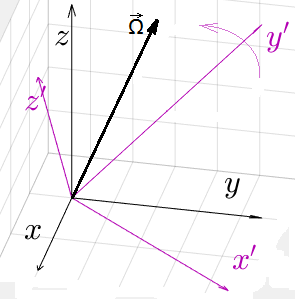
\includegraphics[width=0.7\textwidth,keepaspectratio]{primedframe}
    \caption{The primed reference frame rotating according to the angular velocity vector $\vec{\Omega}$}
    \label{fig:22}
\end{figure}

To start with, let us consider two reference frames, a fixed (unprimed) and a rotating one (primed), such that the latter is rotating about an arbitrary axis with respect to the static one (see Figure~\ref{fig:22}). The rotation is defined by a rotational angular velocity vector $\vec{\Omega}$ and any vector $\vec{V}$ at rest in the rotating frame will have its time rate of change equal to:

\begin{equation}
    \frac{d\vec{V}}{dt} = \vec{\Omega} \times \vec{V}    
\end{equation}

Next, let's consider an arbitrary vector function $\vec{C}(t)$ defined by as $\vec{V}(t) = V_x(t) \hat{x} + V_y(t) \hat{y} + V_z(t) \hat{z}$ in the fixed coordinate system. Alternatively, it can also be expressed in terms of the primed reference frame and it will take the following form: $\vec{V}(t) = V_{x'}(t) \hat{x}(t) + V_{y'}(t) \hat{y}(t) + V_{z'}(t) \hat{z}(t)$. As the two representations refer to the same vector, taking the time derivative of $\vec{V}(t)$ in both forms should yield the same answer, i.e.,

\begin{flalign*}
	\frac{dV_x}{dt}\hat{x} + \frac{dV_y}{dt}\hat{y} + \frac{dV_z}{dt}\hat{z} 
	\, = \, & \frac{dV_{x'}}{dt} \hat{x}'(t) + \frac{dV_{y'}}{dt} \hat{y}'(t) + \frac{dV_{z'}}{dt} \hat{z}'(t) + \\
	& V_{x'}\frac{d\hat{x}'(t)}{dt} + V_{y'}\frac{d\hat{y}'(t)}{dt} + 
	        V_{z'}\frac{d\hat{z}'(t)}{dt}
\end{flalign*}

We know that any vector at rest in the primed coordinate system will have its time derivative with respect to the unprimed system defined as the cross product between the angular velocity vector and itself. As a result, the time derivatives of the unit vectors from the equation above can be written as: $\frac{d\hat{x}'}{dt} = \vec{\Omega} \times \hat{x}'$, $\frac{d\hat{y}'}{dt} = \vec{\Omega} \times \hat{y}'$ and $\frac{d\hat{z}'}{dt} = \vec{\Omega} \times \hat{z}'$.

From here we can write the compact form of our equation as such:

\begin{equation} \label{eq:212}
    \frac{d\vec{V}}{dt} = (\frac{d\vec{V}}{dt})' + \vec{\Omega} \times \vec{V}
\end{equation}

Replacing our arbitrary vector $\vec{V}(t)$ with the magnetic moment $\vec{\mu}$ we get:
\begin{equation} \label{eq:213}
    \frac{d\vec{\mu}}{dt} = (\frac{d\vec{\mu}}{dt})' + \vec{\Omega} \times \vec{\mu}
\end{equation}

From equations \ref{eq:26} and \ref{eq:213} we can write:

\begin{flalign*}
	 (\frac{d\vec{\mu}}{dt})' &= \gamma \vec{\mu} \times \vec{B} - \vec{\Omega} \times \vec{\mu} \Rightarrow \\
	(\frac{d\vec{\mu}}{dt})' &= \gamma \vec{\mu} \times \vec{B} + \vec{\mu} \times \vec{\Omega} \Rightarrow \\
	(\frac{d\vec{\mu}}{dt})' &= \gamma \vec{\mu} \times (\vec{B} + \frac{\vec{\Omega}}{\gamma})
\end{flalign*}

which yields 

\begin{equation} \label{eq:214}
    (\frac{d\vec{\mu}}{dt})' = \gamma \vec{\mu} \times \vec{B}_{eff}
\end{equation}

and therefore shows that in the rotating reference frame the precession motion of the magnetic moment vector can be described according to an 'effective magnetic field' \cite{Haacke1999}. This is a key concept in MRI as it is the basis of magnetic moment analysis in general.

Next, we need to show how to construct this magnetic field so that we can most effectively 'tip' the magnetic moment vector in the transverse plane. It is clear from equation \ref{eq:214} that $\vec{B}_{eff}$ has to have both $x$ and $y$ components in order to move the magnetic moment away from the $z$ axis. For this we can combine our static field $\vec{B}_0 = B_0 \hat{z}$ with a circularly polarised 
rf field $\vec{B}_1^{cir} = B_1(\hat{x} \, cos \omega t - \hat{y} \, sin \omega t) = B_1 \hat{x}'$. By substituting in equation \ref{eq:214} we get:

\begin{equation} \label{eq:215}
    (\frac{d\vec{\mu}}{dt})' = \vec{\mu} \times [\hat{z}'(\omega_0 - \omega) + \hat{x}' \omega_1] = \gamma \vec{\mu} \times \vec{B}_{eff}
\end{equation}

where $\omega_0 = \gamma B_0$ is the Larmor frequency, $\omega$ is the rf field's laboratory frequency and $\omega_1 = \gamma B_1$ is the spin precession frequency generated by $\vec{B}_1^{cir}$.

It is clear from the above equation that an effective 'tipping' around the $\hat{x}'$ axis will happen when the applied rf field's frequency is equal to the Larmor frequency. This leads to the equation of motion of the magnetic moment in the rotating reference frame:

\begin{equation} \label{eq:216}
    (\frac{d\vec{\mu}}{dt})' = \omega_1 \vec{\mu} \times \hat{x}'
\end{equation}

while the condition that accomplishes this:

\begin{equation} \label{eq:217}
    \omega = \omega_0    
\end{equation}

is called the \textit{on-resonance condition}.

In fact, this rotation can be controlled by choosing the amount of time the on-resonance rf field is applied. For a finite amount of time $\tau$, the angle of rotation, called the \textit{flip angle}, can be calculated with the following formula:

\begin{equation} \label{eq:218}
    \Delta \theta = \gamma B_1 \tau
\end{equation}

For example, for a $90^o$ flip angle, the $B_1$ field should have a magnitude of $5.9 \, \mu T$ and be applied for $1.0 \, ms$ for hydrogen protons \cite{Haacke1999}.


%%%%%%%%%%%%%
\subsection{Magnetization, Relaxation and the Bloch Equation}
In the previous subsections, the focus was on a single proton's spin. 
%Also, rotating reference frames and the resonance condition for effectively tipping the magnetic moment were discussed. 
In this subsection, a collection of spins is considered and the interactions with their environment is described. The focus is on the phenomenological Bloch equation that models the relaxation phenomena by means of decay times.

In MRI, as the objects we are imaging are on a macroscopic scale, the next logical step is to consider collections of spins. Therefore, a vector quantity called the \textit{magnetization vector} $\vec{M}(\vec{r},t)$ is now introduced and it is defined as the local magnetic moment per unit volume. Considering a volume $V$ such that all spins residing inside it experience the same external magnetic field, the magnetization is defined as:

\begin{equation} \label{eq:219}
    \vec{M} = \frac{1}{V} \sum_{i \in \text{protons in V}} \vec{\mu}_i
\end{equation}

This set of spins is called an \textit{isochromat} and, ideally, it contains spins which have the same phase. Under these circumstances, extending equation \ref{eq:26} to the volume $V$ we arrive at:

\begin{equation} \label{eq:220}
    \frac{1}{V} \sum_i \frac{d\vec{\mu}_i}{dt} = \frac{\gamma}{V} \sum_i \vec{\mu}_i \times \vec{B}
\end{equation}

which, together with equation \ref{eq:219} yields:

\begin{equation} \label{eq:221}
    \frac{d\vec{M}}{dt} = \gamma \vec{M} \times \vec{B}
\end{equation}
for non-interacting protons.

Decomposing this magnetization vector into parallel and perpendicular components ($\vec{M}_{\parallel} = M_z \hat{z}$ and $\vec{M}_{\perp} = M_x \hat{x} + M_y \hat{y}$) while considering $\vec{B} = B_0 \, \hat{z}$, we arrive at the following two equations:

\begin{equation} \label{eq:222}
    \frac{dM_z}{dt} = 0
\end{equation}

\begin{equation} \label{eq:223}
    \frac{d\vec{M}_{\perp}}{dt} = \gamma \vec{M}_{\perp} \times \vec{B}
\end{equation}

both for non-interacting protons.

It follows now that our next discussion turns to interacting protons. This leads to additional terms in the previous equations which are due to the energy exchange between the spins and their environment, and between themselves. These terms describe different relaxation phenomena because the magnetization vector does not have a fixed magnitude, since it is the sum of individual proton spins. 

At thermal equilibrium and when exposed to a constant, static magnetic field $\vec{B} = B_0 \, \hat{z}$, the magnetization vector is:

\begin{equation} \label{eq:224}
    \vec{M} = M_0 \, \hat{z}
\end{equation}

where $M_0$ is found from quantum statistics to be:

\begin{equation} \label{eq:225}
    M_0 = \frac{\gamma^2 \text{\sout{$h$}}^2 \, B_0 \, \rho}{4 \, K \, T}
\end{equation}

where \sout{$h$} is the reduced Planck constant $h$ ($6.626 \times 10^{-34} J$) or \textit{h-bar} and is equal to $\frac{h}{2 \pi}$, $\rho$ is the number of spins per unit volume (spin density), $K$ is the Boltzmann constant ($1.38 \times 10^{-23} J \, K^{-1}$) and $T$ is the absolute temperature of the system in Kelvin \cite{Haacke1999}. As can be seen from this equation, the only controllable parameter is the external magnetic field's strength, or $B_0$, which in MRI scanners can range between 0.2 to 9 Tesla. 

Now, if the external magnetic field experiences any disturbance, the spin system will be taken out of its initial thermal equilibrium state. However, according to the laws of thermodynamics, the system will return to that state if enough time is given. In MRI, this process can be characterized by two independent relaxation phenomena which are summarized below:

\begin{enumerate}
    \item \textbf{The Spin-Lattice Interaction} which causes the relaxation of the \textit{longitudinal} component of the magnetization vector.
    
    \item \textbf{The Spin-Spin Interaction} which causes the disappearance of the \textit{transverse} component of the magnetization vector.
\end{enumerate}

Under these circumstances, the equations presented above for non-interacting protons have to be changed to accommodate the spin's interaction with their environment. First, the spin-lattice interaction introduces a constant growth rate called $T_1$ which is empirically determined and changes equation \ref{eq:222} to:

\begin{equation} \label{eq:226}
    \frac{dM_z}{dt} = \frac{1}{T_1} (M_0 - M_z) \, \text{ (for } \vec{B}_0 \parallel \hat{z} \text{)}
\end{equation}

with the solution:

\begin{equation} \label{eq:227}
    M_z(t) = M_z(0) e^{-t/T_1} + M_0(1-e^{-t/T_1}) \, \text{ (for } \vec{B}_0 \parallel \hat{z} \text{)}
\end{equation}

Second, the spin-spin interaction introduces a decay rate called $T_2$ which is also empirically determined and which changes equation \ref{eq:223} to:

\begin{equation} \label{eq:228}
    \frac{d\vec{M}_{\perp}}{dt} = \gamma \vec{M}_{\perp} \times \vec{B} - \frac{1}{T_2} \vec{M}_{\perp}
\end{equation}

or 

\begin{equation} \label{eq:229}
    (\frac{d\vec{M}_{\perp}}{dt})' = - \frac{1}{T_2} \vec{M}_{\perp} \, \text{ (in the rotating frame)} 
\end{equation}

with the solution:

\begin{equation} \label{eq:230}
    \vec{M}_{\perp}(t) = \vec{M}_{\perp}(0) e^{-t/T_2} \, \text{ (in the rotating frame)}
\end{equation}
The two solutions are shown in Figure \ref{fig:relax}.

\begin{figure}[ht]
    \centering
    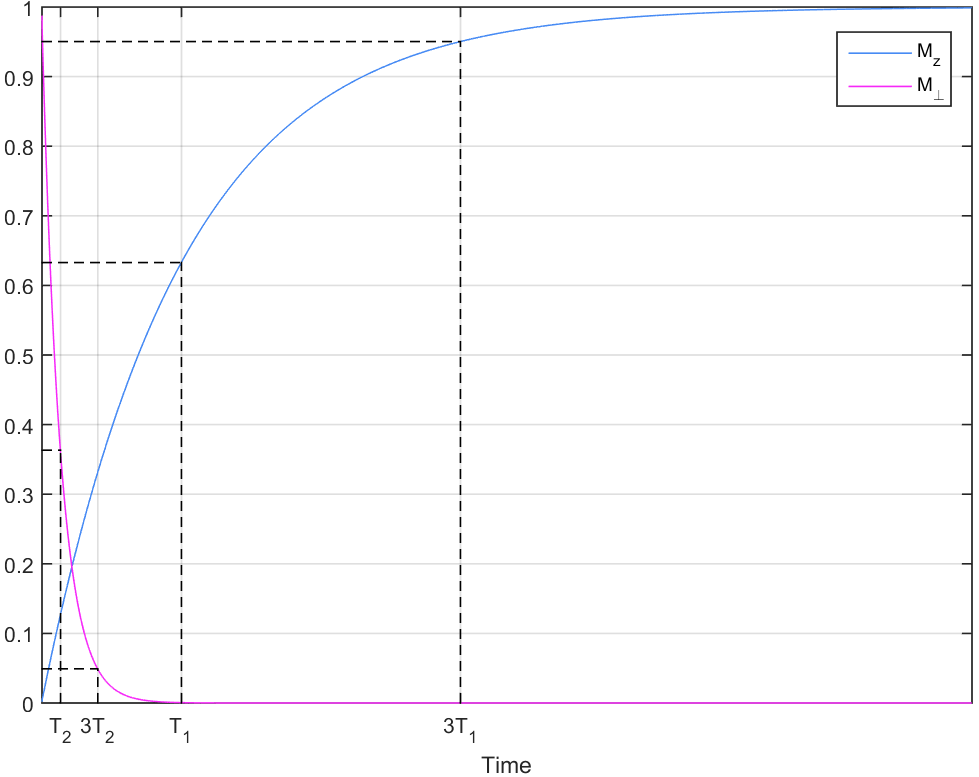
\includegraphics[width=1\textwidth,keepaspectratio]{MzMt}
    \caption{The regrowth of the longitudinal magnetization from $0$ to its initial value $M_z$ and the decay of the transverse magnetization from an initial value $M_{\perp}(0)$ to $0$} 
    \label{fig:relax}
\end{figure}

% \begin{figure}
%     \centering
    
%     \begin{subfigure}[b]{0.48\textwidth}
%         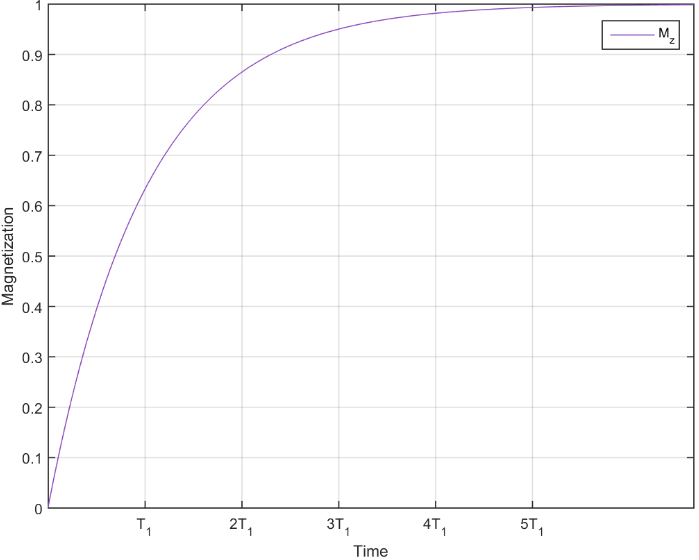
\includegraphics[width=\textwidth]{Mpara}
%         \caption{The regrowth of the longitudinal magnetization from $0$ to its initial value $M_z$}
%         \label{fig:Mpara}
%     \end{subfigure}
%     ~ %add desired spacing between images, e. g. ~, \quad, \qquad, \hfill etc. 
%       %(or a blank line to force the subfigure onto a new line)
%     \begin{subfigure}[b]{0.48\textwidth}
%         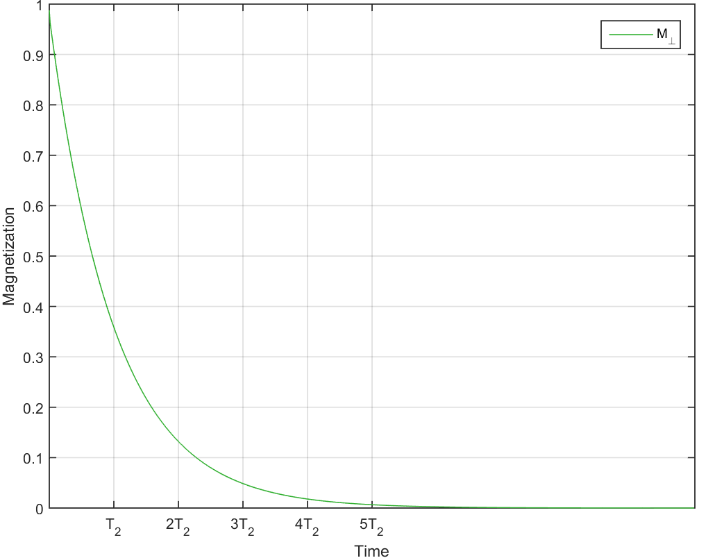
\includegraphics[width=\textwidth]{Mperp}
%         \caption{The decay of the transverse magnetization from an initial value $M_{\perp}(0)$ to $0$}
%         \label{fig:Mprep}
%     \end{subfigure}
    
    
%     \caption{TODO: Write caption text AND Label y axis with Mz(0) Mtr(0) and so on. See fig 4.1 book} 
%     \label{fig:relax}
% \end{figure}

Actually, the transverse relaxation happens at a higher rate because of additional field inhomogeneities which cause the spins to dephase faster. This is characterised by a separate decay time called $T_2'$. We can therefore define the total relaxation rate $R_2^*$ as the sum between the internal ($R_2$) and external ($R_2'$) relaxation rates: $R_2^* = R_2 + R_2'$. This yields the following relation between the relaxation times:

\begin{equation} \label{eq:231}
    \frac{1}{T_2^*} = \frac{1}{T_2} + \frac{1}{T_2'}
\end{equation}

It is noteworthy to mention that the loss of phase due to external field inhomogeneities can be recovered by means of an \textit{echo} which can be achieved under certain circumstances, while the intrinsic $T_2$ losses are not recoverable. 

It follows that an equation which combines both types of processes is defined. This one vector equation is called \textit{the Bloch equation} and is presented below:
\begin{equation} \label{eq:232}
    \frac{d\vec{M}}{dt} = \gamma \vec{M} \times \vec{B} + \frac{1}{T_1} (M_0 - M_z) \hat{z} - \frac{1}{T_2} \vec{M}_{\perp}
\end{equation} 
which, for $\vec{B} = B_0 \hat{z}$, has the following solutions:
\begin{equation} \label{eq:233}
    \frac{dM_z}{dt} = \frac{M_0 - M_z}{T_1}
\end{equation}
\begin{equation} \label{eq:234}
    \frac{dM_x}{dt} = \omega_0 M_y - \frac{M_x}{T_2}
\end{equation}
\begin{equation} \label{eq:235}
    \frac{dM_x}{dt} = -\omega_0 M_x - \frac{M_y}{T_2}
\end{equation}
where $\omega_0 = \gamma B_0$.

\begin{figure}[ht]
    \centering
    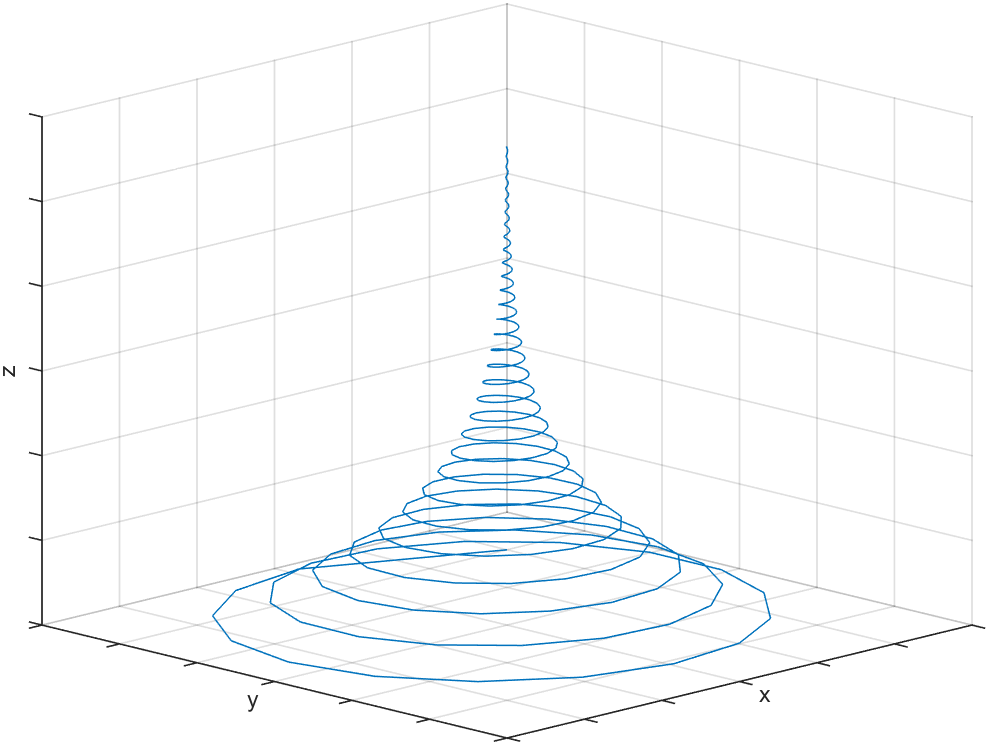
\includegraphics[width=1\textwidth,keepaspectratio]{spiral}
    \caption{The trajectory of the tip of the magnetization vector showing at the same time the regrowth and the decay of its components.}
    \label{fig:spiral}
\end{figure}

Furthermore, the three differential equations presented above have the following solutions in \textit{Cartesian representation}:
\begin{equation} \label{eq:236}
    M_x(t) = e^{-t/T_2} (M_x(0) \, cos \, \omega_0 t + M_y(0) \, sin \, \omega_0 t)
\end{equation}
\begin{equation} \label{eq:237}
    M_y(t) = e^{-t/T_2} (M_y(0) \, cos \, \omega_0 t - M_x(0) \, sin \, \omega_0 t)
\end{equation}
\begin{equation} \label{eq:238}
    M_z(t) = M_z(0) e^{-t/T_1} + M_0 (1 - e^{-t/T_1})
\end{equation}
with the following steady-state solutions: $M_x(\infty) = M_y(\infty) = 0$ and $M_z(\infty) = M_0$.

A graphical representation of the magnetization vector components evolution throughout time for a white matter tissue sample with $T_1 = 600 \, ms$ and $T_2 = 80 \, ms$, placed in a constant magnetic field of strength $B = 7 \, T$ can be found in Figure~\ref{fig:MxMyMz}, while the three dimensional representation of how the magnetization vector reaches its equilibrium state can be seen in Figure~\ref{fig:spiral}.

\begin{figure}[ht]
    \centering
    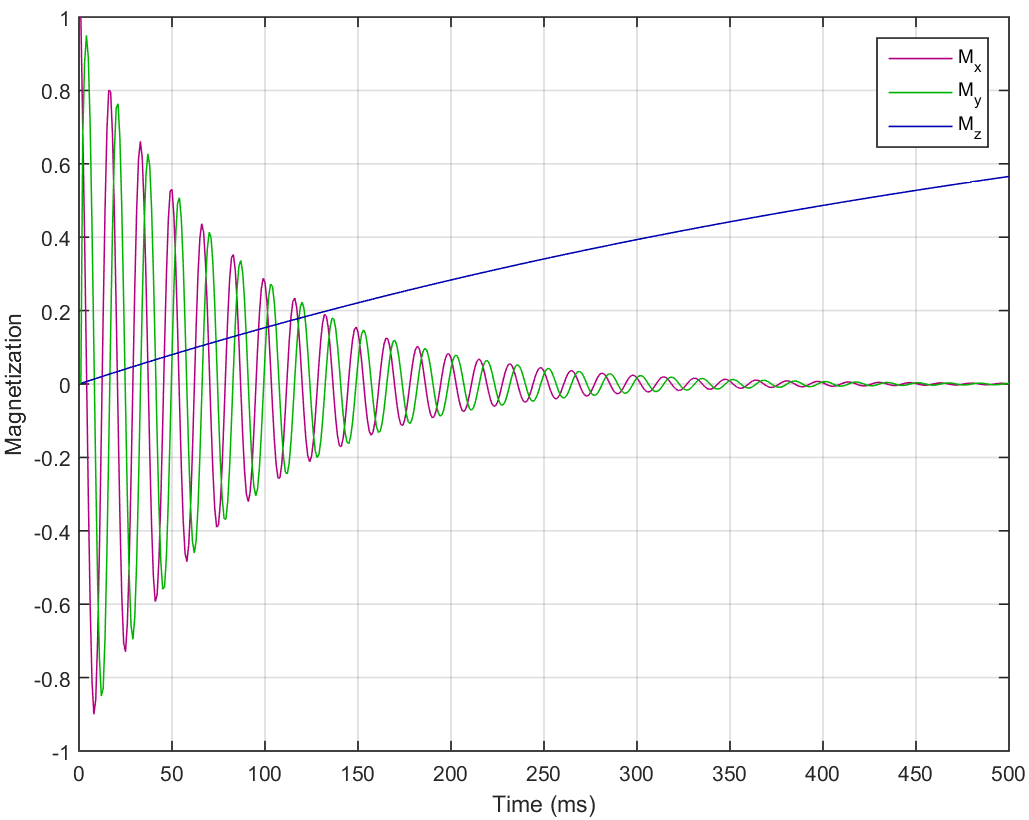
\includegraphics[width=1\textwidth,keepaspectratio]{MxMyMz}
    \caption{The regrowth of the longitudinal $M_z$ component of the magnetization vector from $0$ to its initial value $M_0$ shown in blue and the decay of both transverse components $M_x$ and $M_y$ from an initial value to 0 shown in purple and green. $M_0$ is considered to be equal to $1$ for illustration purposes.}
    \label{fig:MxMyMz}
\end{figure}

The vector components can also be viewed in \textit{matrix representation}. First, the rotation matrix about the z axis in a clockwise fashion is defined as:

\begin{equation}
    R_z ( \theta ) = \left[
    \begin{array}{c c c}
          cos \theta & sin \theta & 0 \\
        - sin \theta & cos \theta & 0 \\
           0         &  0         & 1 
    \end{array}
    \right]
\end{equation}

Second, the decay factors are placed in matrix form as well:

\begin{equation}
    A ( t ) = \left[
    \begin{array}{c c c}
          e^{-t/T_2} &     0      &     0 \\
              0      & e^{-t/T_2} &     0 \\
              0      &     0      & e^{-t/T_1}
    \end{array}
    \right]
\end{equation}

and

\begin{equation}
    B ( t ) = \left[
    \begin{array}{c}
        0 \\
        0 \\
    M_0(1 - e^{-t/T_1})
    \end{array}
    \right]
\end{equation}

Finally, we can write the solution as:

\begin{equation} \label{eq:242}
    M(t) = A(t) R_z(\omega_0 t) M(0) + B(t)
\end{equation}

where $M(t)$ is:

\begin{equation}
    M ( t ) = \left[
    \begin{array}{c}
        M_x(t) \\
        M_y(t) \\
        M_z(t)
    \end{array}
    \right]
\end{equation}

A final representation can also be considered and it is called the \textit{complex representation} of the transverse magnetization. Its notation is:

\begin{equation}
    M_{+} \equiv M_x(t) + i M_y(t)
\end{equation}

By using equations \ref{eq:236} and \ref{eq:237} we get:

\begin{flalign*}
    M_{+}(t) &= e^{-t/T_2} (M_x(0) \, cos \, \omega_0 t + M_y(0) \, sin \, \omega_0 t) \\
             &+ i \, e^{-t/T_2} (M_y(0) \, cos \, \omega_0 t - M_x(0) \, sin \, \omega_0 t) \\
             &= e^{-t/T_2} \, [  M_x(0) (cos \omega_0 t - i \, sin \omega_0 t) + 
                            i \, M_y(0) (cos \omega_0 t - i \, sin \omega_0 t) ] 
\end{flalign*}

which yields:

\begin{equation} \label{eq:245}
    M_{+}(t) = e^{-t/T_2} M_{+}(0) e^{-i \omega_0 t}
\end{equation}

The complex form is useful when characterizing imaging signals. Therefore, by defining $M_{+}(t) = \lvert M_{+}(t) \rvert e^{i \phi(t)}$, where $\phi(t) = - \omega_0 t + \phi (0)$, equation \ref{eq:245} becomes:

\begin{equation} \label{eq:246}
    M_{+}(t) = \lvert M_{+}(0) \rvert e^{-t/T_2 \, -i (\omega_0 t - \phi(0))}
\end{equation}

which is the solution of the transverse magnetization in complex representation.



%%%%%%%%%%%%%%%%%%%%%%%%%%
\section{Image Formation}
The discussion so far was centered around the physical principles of nuclear magnetic resonance. The next step is to describe how MRI images are obtained, from signal acquisition to image reconstruction. 

%%%%%%%%%%%%%
\subsection{Signal Detection}
A crucial part of Magnetic Resonance Imaging is the signal detection process. This happens once the magnetization vector has been tipped away from the equilibrium position and it starts to relax back. The basic principle behind this process comes from \textit{Faraday's law of induction} which states that an electromotive force will be created in a coil through which a magnetic flux sweeps \cite{Haacke1999}. This force is equal to the rate at which the magnetic flux $\Phi(t)$ passing through the receiver coil is changing in time:
\begin{equation} \label{eq:247}
    emf = - \frac{d \Phi(t)}{dt}
\end{equation}
where 
\begin{equation}
    \Phi(t) = \int_{sample} \vec{B}^{receive}(\vec{r}) \cdot \vec{M}(\vec{r}, t) d\vec{r}
\end{equation}
and $\vec{B}^{receive}(\vec{r})$ is the 'received' magnetic field produced by the RF detection coil, while $\vec{M}(\vec{r}, t)$ is the magnetization vector at position $\vec{r}$ and time $t$.

The signal produced by the receiver coil is proportional to $emf$ found in equation \ref{eq:247} and has the following form:
\begin{equation}
    S(t) \propto - \frac{d}{dt} 
    \int_{sample}
          [B_x^{receive} (\vec{r}) M_x (\vec{r}, t) + 
          B_y^{receive} (\vec{r}) M_y (\vec{r}, t) + 
          B_z^{receive} (\vec{r}) M_z (\vec{r}, t)]  d\vec{r}
\end{equation}
for a sample that is placed in a static constant field $\vec{B} = B_0 \hat{z}$, after an RF pulse has been applied and the magnetization vector has all three components: $M_x$, $M_y$ and $M_z$.

Turning to the magnetization vector components described in the previous section in equations \ref{eq:238} and \ref{eq:246}, it follows that the solutions can be written for each position $\vec{r}$ in the sample:
\begin{equation}
    M_z(\vec{r}, t) = M_z(\vec{r}, 0) e^{-t/T_1(\vec{r})} + M_0 (1 - e^{-t/T_1(\vec{r})})
\end{equation}
and
\begin{equation}
    M_{+}(\vec{r}, t) = M_{\perp}(\vec{r},0) e^{-t/T_2(\vec{r})} e^{-i (\omega_0 t - \phi(\vec{r}))}
\end{equation}
where the transverse components can be recovered with $M_x = Re (M_{+})$ and $M_y = Im (M_{+})$.

Taking the time derivative of the two equations the following 2 equations are found:
\begin{equation}
    \frac{d}{dt} M_z(\vec{r}, t) = 
        - \frac{1}{T_1} M_z (\vec{r}, 0) e^{-t/T_1(\vec{r})} 
        - \frac{1}{T_1} M_0 (1 - e^{-t/T_1(\vec{r})})
\end{equation}
and
\begin{equation}
    \frac{d}{dt} M_{+}(\vec{r}, t) = 
        - \frac{1}{T_2} M_{\perp}(\vec{r},0) e^{-t/T_2(\vec{r})} e^{-i (\omega_0 t - \phi(\vec{r}))}
        - i \omega_0  M_{\perp}(\vec{r},0) e^{-t/T_2(\vec{r})} e^{-i (\omega_0 t - \phi(\vec{r}))}
\end{equation}

Because the Larmor frequency $\omega_0$ is at least four orders-of-magnitude higher than $1/T_1$ and $1/T_2$  \cite{Haacke1999}, the derivative of $e^{-t/T_1}$ and $e^{-t/T_2}$ can be neglected giving the signal, $S(t)$, as:
\begin{equation} \label{eq:254}
\begin{split}
    S(t) \propto \, 
        \omega_0 \int_{sample} e^{-t/T_2(\vec{r})} M_{\perp}(\vec{r},0) 
            [& B_x^{receive}(\vec{r}) sin(\omega_0 t - \phi_0(\vec{r})) \\
           + & B_y^{receive}(\vec{r}) cos(\omega_0 t - \phi_0(\vec{r})) ] d\vec{r}
 \end{split}
\end{equation}

Writing $B_x^{receive}(\vec{r}) \equiv B_{\perp} cos(\theta_B)$ and $B_y^{receive}(\vec{r}) \equiv B_{\perp} sin(\theta_B)$ with $\theta_B$ being the angle of reception and $B_{\perp}$ the magnitude of the $xy$ receive field \cite{Haacke1999}, equation \ref{eq:254} becomes:

\begin{equation}
    S(t) \propto
        \omega_0 \int_{sample} e^{-t/T_2(\vec{r})} M_{\perp}(\vec{r},0) 
            B_{\perp}(\vec{r}) sin(\omega_0 t + \theta_B(\vec{r}) - \phi_0(\vec{r})) d\vec{r}
\end{equation}
which can be modified to incorporate external field inhomogeneities by replacing $T_2$ with $T_2^*$.

Next, the oscillations at the frequency $\omega_0$ are removed by a process called \textit{demodulation} \cite{Haacke1999}. This transforms the previous signal expression in the following one:
\begin{equation} \label{eq:256}
    S(t) \propto
        \omega_0 \int_{sample} e^{-t/T_2(\vec{r})} M_{\perp}(\vec{r},0) 
            B_{\perp}(\vec{r}) e^{i(\phi_0(\vec{r}) + \theta_B(\vec{r}))} d\vec{r}
\end{equation}

Considering the signal in complex representation $s(t) \equiv s_{re}(t) + i s_{im}(t)$, where $s_{re}$ and $s_{im}$ are the real and imaginary channel demodulated signals and writing the receive field in complex form as well $B_{+} \equiv B_x^{receive} + i B_y^{receive} = B_{\perp} e^{i \theta_B}$, equation \ref{eq:256} becomes:

\begin{equation} \label{eq:257}
    S(t) \propto
        \omega_0 \int_{sample} M_{+}(\vec{r}, t) B_{+}^* (\vec{r}) d\vec{r}
\end{equation}



%%%%%%%%%%%%%
\subsection{K-Space Construction}
The acquired MRI signal discussed previously represents the global signal coming from the tissue sample. Therefore, a way to determine the spatial distribution of the signal is needed. This is done by a combination of gradients applied to the main magnetic field which will make the spins precess at different rates and acquire different phases. The information is then stored in a matrix form called \textit{k-space} which represents the Fourier coefficients of the image.

These gradients can be applied on each of the three directions or on any combination of them. The gradient field is defined by:
\begin{equation}
    \begin{split}
        \vec{G}(t) & \equiv \nabla B_{G_z}(\vec{r}, t) \\
                   &    =   \frac{\partial B_{G_z}(\vec{r},t)}{\partial x} \hat{x} + \frac{\partial B_{G_z}(\vec{r},t)}{\partial y} \hat{y} + \frac{\partial B_{G_z}(\vec{r},t)}{\partial z} \hat{z} \\
                   & \equiv G_x(t) \hat{x} + G_y(t) \hat{y} + G_z(t) \hat{z}
    \end{split}
\end{equation}

which leads to the following equation for the total magnetic field:

\begin{equation}
    \vec{B}(\vec{r},t) = (B_0 + B_{G_z}(\vec{r}, t))\hat{z} = (B_0 + G_x(t)x + G_y(t)y + G_z(t)z) \hat{z} = (B_0 + \vec{G}(t) \cdot \vec{r}) \hat{z}
\end{equation}

In terms of the angular frequency of the precessing spins which are now placed in a spatially varying magnetic field, the formula changes to:

\begin{equation} \label{eq:260}
    \omega(\vec{r}, t) = \gamma \lvert \vec{B}(\vec{r}, t) \rvert = \gamma B_0 + \gamma B_{G_z} (\vec{r}, t) = \omega_0 + \gamma \vec{G}(t) \cdot \vec{r}
\end{equation}

Equation \ref{eq:260} is of utmost importance in MRI as it makes the connection between spatial coordinates and frequency of precession.

As a consequence, the first step towards image formation is done by spatially varying the main magnetic field in the z-axis. This is called the \textit{slice-select gradient ($G_z \hat{z}$)} and it will make the protons spin at different frequencies in that direction  \cite{Haacke1999}. Applying an RF pulse of frequency $\omega_0$ will now excite only the spins whose positions are at $z_0$. In practice, an infinitely small slice is not achievable, and therefore we talk about \textit{slice thickness}. This is achieved by applying sinc RF pulses of certain frequency bandwidths $\Delta \omega_0$, which have the nice property of selecting a range of frequencies of corresponding thickness $\Delta z_0$. This can be seen in Figure \ref{fig:sliceselect}. 

\begin{figure}[ht]
    \centering
    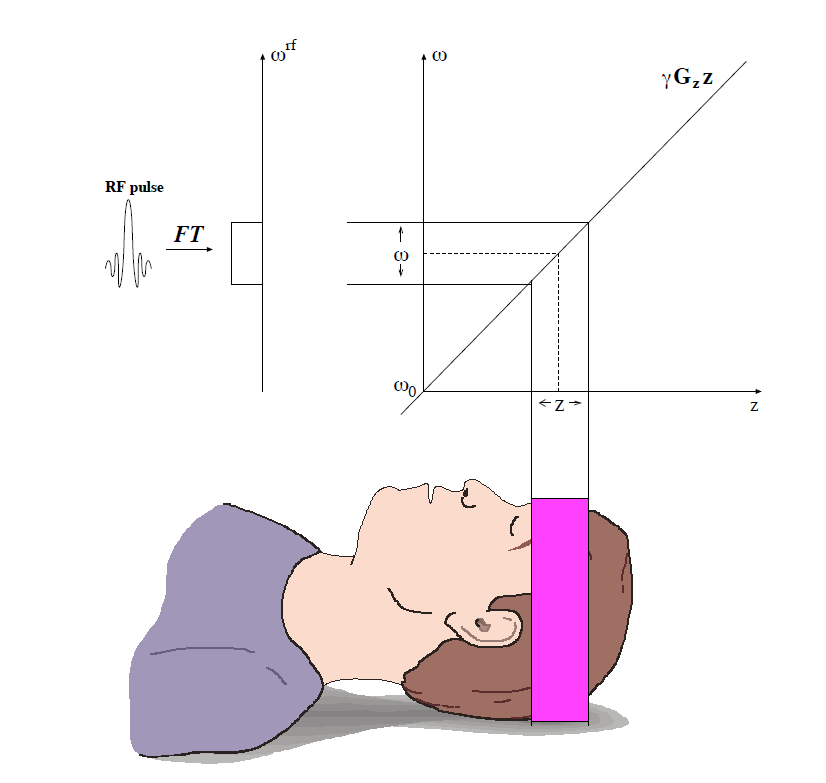
\includegraphics[width=1\textwidth,keepaspectratio]{sliceselect}
    \caption{Slice selection is shown in this image for a slice in the x-y plane. The slice select gradient ($G_z$) is applied along the z-axis. The RF pulse of frequency bandwidth $\Delta \omega$ will excite the protons precessing at this frequency range. Figure courtesy of \cite{Drobnjak07}}
    \label{fig:sliceselect}
\end{figure}

The second step is called \textit{spatial information encoding} and it is done after the RF pulse has excited a slice. Throughout the relaxation period, the Bloch equations will take the following form:

\begin{equation} \label{eq:258}
    \frac{dM_z}{dt} = \frac{M_0 - M_z}{T_1}
\end{equation}
\begin{equation} \label{eq:259}
    \frac{dM_x}{dt} = ( \omega_0 + \gamma \vec{G}(t) \cdot \vec{r} ) M_y - \frac{M_x}{T_2}
\end{equation}
\begin{equation} \label{eq:260}
    \frac{dM_x}{dt} = - (\omega_0 + \gamma \vec{G}(t) \cdot \vec{r}) M_x - \frac{M_y}{T_2}
\end{equation}

The solution for these equations will also include an accumulation in phase $\phi(\vec{r}, t) = - \int_0^t \omega(\vec{r}, t') dt' = -\omega_0 t - \gamma \int_0^t \vec{r} \cdot \vec{G}(t') dt'$. Thus, the solution in complex representation for the transverse magnetization will be:

\begin{equation}
    M_{+}(\vec{r},t) = \lvert M_{+}(\vec{r},0) \rvert e^{-t/T_2(\vec{r}) \, -i (\omega_0 t + \gamma \int_0^t \vec{r} \cdot \vec{G}(t') dt')}
\end{equation}

Considering the slice selection gradient being in the z direction, only x- and y-gradients are needed to encode spatial information in the selected slice. This information can be found in the spatial frequency of the detected signal:

\begin{equation}
    S(t) = \int \int 
            e^{-t/T_2(\vec{r})} M_{\perp}(\vec{r},0) 
                B_{\perp}(\vec{r}) 
                e^{ -i \gamma \int_0^t G_x(t')x + G_y(t')y dt'} dx dy
\end{equation}

This signal is collected during \textit{read out} as uniformly spaced time points \cite{Haacke1999} and stored in a matrix called the \textit{k-space}, where:
\begin{equation}
    k_x(t) = \frac{\gamma}{2 \pi} \int_0^t \vec{G}_x(t') dt' 
    \qquad\text{and}\qquad
    k_y(t) = \frac{\gamma}{2 \pi} \int_0^t \vec{G}_y(t') dt' 
\end{equation}
which, for constant gradients become:
\begin{equation}
    k_x(t) = \frac{\gamma}{2 \pi} G_x t
    \qquad\qquad\text{and}\qquad\qquad
    k_y(t) = \frac{\gamma}{2 \pi} G_y t
\end{equation}

Now, not taking into consideration the decay term $e^{-t/T_2(\vec{r})}$ during signal collection and using equation \ref{eq:225} to introduce the spin density of the sample, the signal in terms of k-space becomes:
\begin{equation}
    S(k_x, k_y) = \int \int \rho(x,y) e^{-i 2 \pi (k_x x + k_y y)} dx dy
\end{equation}

A visual representation of the k-space can be found in Figure~\ref{fig:kspace}. Note that k-space undergoes a Fourier transform in order to obtain the final image as seen in Figure~\ref{fig:reconstruction}.

Generally, k-space data is acquired line by line. Other techniques do exist, but they will not be discussed in this thesis. Every k-space line is a new repetition of the undergoing MRI sequence with a different phase-encoding step. This results in a total acquisition time ($T_A$) of:

\begin{equation}
    T_A = T_R \times N_{PE}
\end{equation}

where $T_R$ is the repetition time and $N_{PE}$ is the number of phase-encoding steps.

\begin{figure}[H]
    \centering
    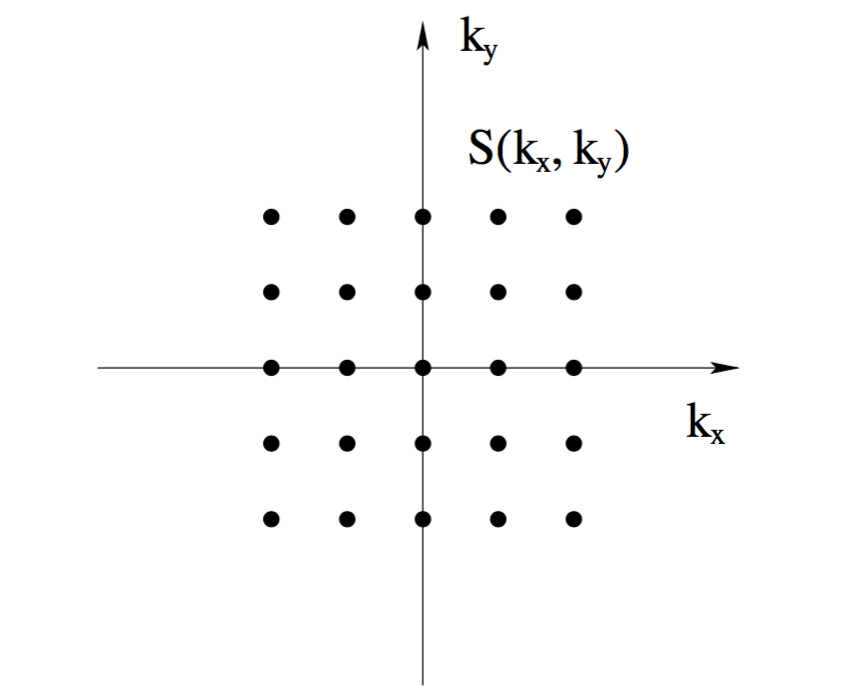
\includegraphics[width=.8\textwidth,keepaspectratio]{kspace}
    \caption{An example of a 4x4 k-space. Figure courtesy of \cite{Drobnjak07}}
    \label{fig:kspace}
\end{figure}

%%%%%%%%%%%%%
\subsection{Image Reconstruction}
We have seen so far how k-space is being constructed. The main steps are: first, by spatially varying the magnetic field and thus allowing for different frequencies and phases into spin's precessing behaviour, we encode spatial information into collections of spins. Second, the signal coming from the selected slice is sampled and a line of k-space is filled in with the corresponding Fourier coefficients. Third, the sequence is repeated with different phase-encoding steps until all lines of k-space are filled in. Once all the data has been collected, the Fourier transform is used to transform the k-space into an image (Figure~\ref{fig:reconstruction}). 

The distance between two adjacent points in k-space is called $\Delta k_x$ and $\Delta k_y$, depending on the direction (phase-encoding or frequency-encoding). These sampling intervals are inversely proportional to the image field-of-view (FOV) \cite{Deshmane2012}. This means that an increase in $\Delta k$ will lead to a decrease in the field-of-view in that direction. The highest spatial frequencies sampled in k-space are called $k_{x,max}$ and $k_{y,max}$ and they are inversely proportional to the resolution of the image (i.e. distance between consecutive points in the image: $\Delta x$ and $\Delta y$). Again, this means that by increasing $k_{x,max}$ or $k_{y,max}$ the distances will decrease and therefore the resolution of the final image will be higher. In conclusion, the final MR image characteristics are dependent upon the number of k-space points and the distance between them, all of which can be manipulated to obtain the desired image. 

\begin{figure}[ht]
    \centering
    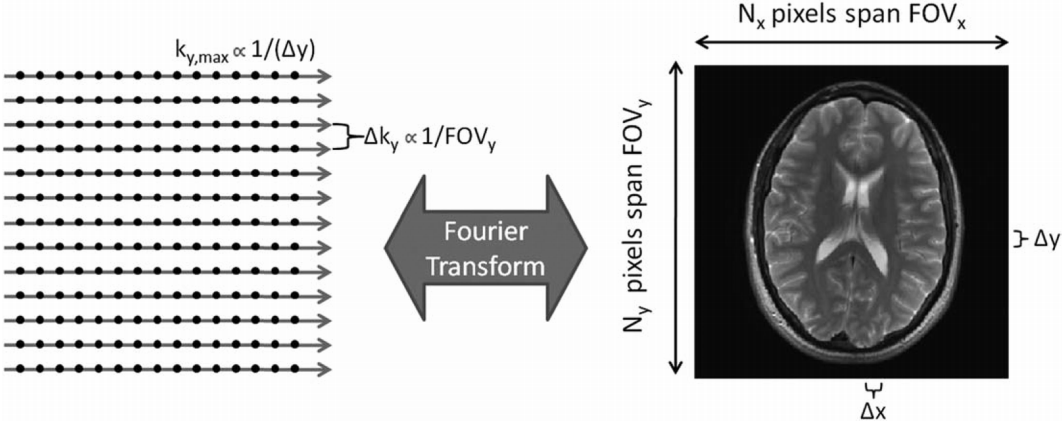
\includegraphics[width=1\textwidth,keepaspectratio]{reconstruction}
    \caption{A cartesian k-space undergoing a Fourier Transform to obtain the final image. Figure courtesy of \cite{Deshmane2012}}
    \label{fig:reconstruction}
\end{figure}

The main relationships discussed so far are presented in a mathematical form in equations \ref{eq:269}, \ref{eq:270}, \ref{eq:272} and \ref{eq:273}. The relationship between FOV and the sampling intervals are shown in the following two equations:

\begin{equation} \label{eq:269}
    FOV_x = \frac{1}{\Delta k_x} = \frac{1}{\frac{\gamma}{2 \pi} G_x \Delta t}
\end{equation}
and
\begin{equation} \label{eq:270}
    FOV_y = \frac{1}{\Delta k_y} = \frac{1}{\frac{\gamma}{2 \pi} \Delta G_y t_y}
\end{equation}

while the spatial resolution of the image is related to the highest spatial frequencies sampled in k-space by:

\begin{equation} \label{eq:272}
    \Delta x = \frac{1}{N_x \Delta k_x} = \frac{1}{2 k_{x,max}} = \frac{1}{\frac{\gamma}{2 \pi} G_x T}
\end{equation}
and
\begin{equation} \label{eq:273}
    \Delta y = \frac{1}{N_y \Delta k_y} = \frac{1}{2 k_{y,max}} = \frac{1}{\frac{\gamma}{2 \pi} 2 G_{y,max} t_y}
\end{equation}

A more interesting discussion arises when k-space data are missing. This can happen if the sampling rate is not high enough (at least twice as fast as the highest frequency component contained within the MRI signal) to reconstruct the signal. This is called the \textit{Nyquist-Shannon} theorem and if it is broken an interesting artefact occurs called \textit{aliasing} \cite{Deshmane2012}. A nice depiction of this phenomenon can be seen in Figure~\ref{fig:partialkspace} where the rightmost column shows what happens when undersampling occurs in the phase-encoding direction.

\begin{figure}[ht]
    \centering
    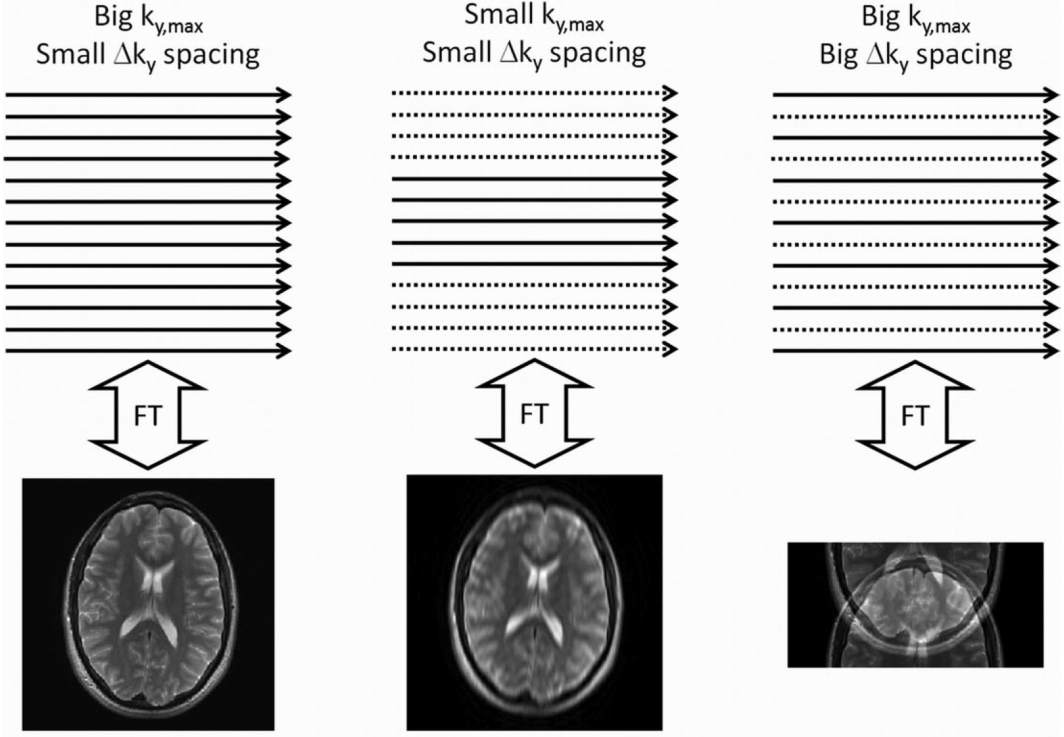
\includegraphics[width=1\textwidth,keepaspectratio]{partialkspace}
    \caption{The left column shows a fully sampled k-space which will yield a high-resolution image. The middle column shows what happens to the final image when higher frequencies are discarded ($k_{y,max}$ is decreased). This will yield a lower resolution image, but keep the same FOV. The last column shown an aliased image example which happened because $\Delta k_y$ was increased while $k_{y,max}$ was kept constant. Figure courtesy of \cite{Deshmane2012}}
    \label{fig:partialkspace}
\end{figure}

Mathematically, this can be explained with the following deduction. We start from the relationship between $\Delta k$ and FOV for the case shown in the left side of Figure~\ref{fig:partialkspace}: $\Delta k_y = \frac{1}{FOV_y}$. By missing every other line of k-space we basically increase the spacing twofold. Therefore, let's consider this new relationship as $\Delta k_y' = \frac{1}{FOV_y'}$. But, we also know that:

\begin{flalign*}
    \Delta k_y' = 2 \Delta k_y = \frac{2}{FOV_y} = \frac{1}{\frac{FOV_y}{2}} = \frac{1}{FOV_y'}
\end{flalign*}

Therefore, our new field-of-view is half of the previous one $FOV_y' = \frac{FOV_y}{2}$. This leads to aliasing as the missing FOV folds itself on top of the halved one. This theoretical consideration is important to remember for the next section where Parallel Imaging techniques are introduced as a means of reducing the amount of time a scan requires by reducing the number of phase-encoding steps and resolving the aliasing that inevitably happens.

%%%%%%%%%%%%%%%%%%%%%%%%%%
\section{Parallel Imaging}

%%%%%%%%%%%%%
\subsection{Motivation}
We have discussed so far about the basic steps needed to acquire MR images, from the physics of spins precessing in magnetic fields to image reconstruction from k-space data. However, one topic that has not been fully addressed was the imaging time. Indeed, an MRI scan is a procedure that can take from a few minutes to a few hours depending on the characteristics of the resulting images. As can be expected, a way to reduce the scan time is a nice to have requirement for both patient comfort and reduced movement artefacts. 

For this reason, in the late 1980s, fast imaging sequences such as \textit{Echo Planar Imaging (EPI)} or \textit{Fast Low-Angle Shot (FLASH)} were invented. Both FLASH \cite{Haase1986} and EPI \cite{DeLaPaz1994} manage to reduce the imaging time per slice to a few tens of milliseconds which leads to imaging full volumes in a couple of seconds and limit the possibility of movement during acquisition. However, pushing the imaging time even further down becomes problematic as the hardware components face technical limitations when it comes to rapidly switching on and off the gradients. Also, patient safety is at risk when gradient strengths and slew rates exceed certain thresholds. 

Under these circumstances, new techniques had to be implemented to overcome these limitations. This is how \textit{parallel acquisition techniques} came into being. These are not new imaging sequences, but they are a collection of reconstruction algorithms that can be applied to almost all existing imaging sequences without changing the scanner's hardware behaviour.  

Actually, the main idea behind \textit{Parallel MRI (pMRI)} is to replace phase-encoding steps from k-space data with rf coil information. The coil data comes from a collection of receivers working in parallel (simultaneously). Their spatial sensitivity profiles can be used to undersample k-space, which translates into skipping some time-consuming phase-encoding steps. As a result, the acquisition time is reduced by a so called \textit{acceleration factor R}, while the reconstruction algorithms take the time-consuming burden. 

Undoubtedly, there are many advantages that parallel imaging techniques bring. Some of them are worth mentioning:
\begin{itemize}
    \item Real-time imaging
    \item Less artifacts caused by movement
    \item Shorter periods for holding one's breath
    \item Less contrast agent in MR angiographies
\end{itemize}

All in all, pMRI is widely used in clinics nowadays and so a closer look at how they work and on what principles they are based upon is worthwhile. This will be the subject of the next subsections where basic concepts are presented and one of the algorithms is presented in more depth.

%%%%%%%%%%%%%
\subsection{Basic Concepts}
Parallel Imaging is used in MRI in order to reduce scanning time. This is possible because time-consuming phase-encoding steps are skipped during the scan. Unfortunately, this means that the final images will be aliased. The purpose of pMRI techniques is, therefore, to resolve the 'folding' and to provide clinicians with good data sets. Currently, there are a few approaches to this issue, but before mentioning them it is worth discussing about what they all have in common:

\begin{enumerate}

    \item For all available techniques k-space data are undersampled in the phase-encoding direction. As a result, the definition of the acceleration factor is $R = \frac{\text{number of lines for a fully sampled k-space}}{\text{number of lines for the undersampled k-space}}$ \cite{Deshmane2012}. For example, skipping every other line of k-space results in an acceleration factor $R = 2$.
    
    \item Imaging is done using an array of coils whose sensitivity profiles are acquired during a prescan at the beginning of the MRI examination. Because the coils do not have a homogeneous sensitivity map, but they are rather more sensitive to the signal originating from the tissue mass which is located more closely to the coil, they add an extra source of spatial information for the reconstruction step.
    
    \item An algorithm reconstructs the final unaliased, full FOV image by using the undersampled data and the individual coil sensitivities.
    
\end{enumerate}

\begin{figure}[ht]
    \centering
    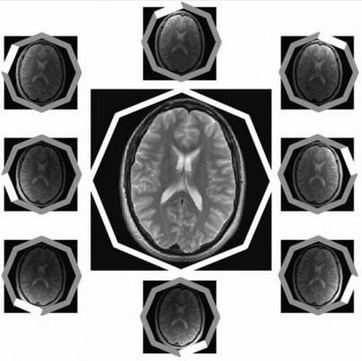
\includegraphics[width=.7\textwidth,keepaspectratio]{coils}
    \caption{This image shows an example of an 8-channel array, with the coils distributed around the object of interest. Figure courtesy of \cite{Deshmane2012}}
    \label{fig:coils}
\end{figure}

As it is evident by now, in pMRI techniques an important actor is the coil. This piece of hardware is more commonly known as \textit{the multichannel receiver array} as it is made up of a series of receiver coils which are uniformly distributed around the organ of interest. Any of the individual channels are more sensitive to the signal coming from an area closer to it and less sensitive as the distance increases.

Clinically, the multicoil receiver array contains from 4 to more than 32 channels that have their own associated sensitivity profiles. They can be arranged either linearly as it happens for spine MR imaging, or radially as it is more common for neuroimaging. An example of how 8 coils could be circularly placed is seen in Figure~\ref{fig:coils}. As the reconstruction algorithm relies on extra information brought by the coils' sensitivity maps, i.e. the sensitivity differences that exist between coils, the acceleration can only take place in the direction of the receiver array. This means that, in practice, there is a lot of thought put behind the placement of these channels such that the final configuration provides the maximum possible acceleration in the phase-encoding direction. Moreover, any overlap between the sensitivity profiles is avoided as much as possible.

\begin{figure}[ht]
    \centering
    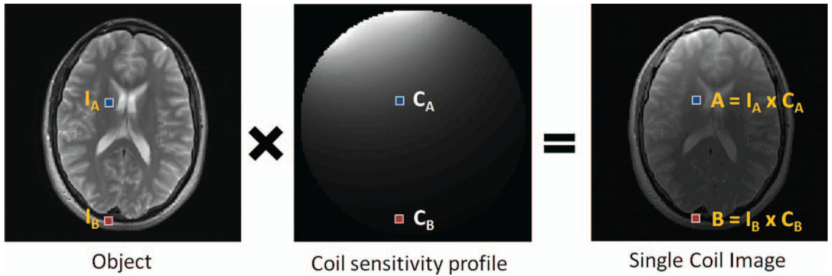
\includegraphics[width=\textwidth,keepaspectratio]{onecoilsens}
    \caption{A single coil image is obtained by 'weighting' the coil sensitivity profile with the object image. Figure courtesy of \cite{Deshmane2012}}
    \label{fig:onecoilsens}
\end{figure}

Turning to an individual coil, an MR image which could possibly result is shown in Figure~\ref{fig:onecoilsens}. The mathematical interpretation of how the final image looks when the signal was collected by a receiver coil which has an associated sensitivity map (as shown in the middle image) is that every voxel in the final image will be 'weighted' by the corresponding sensitivity index. As such, the 2 locations, A and B, from the final MR image can be thought of as having intensity values which result from multiplying the coil sensitivity at location A with the actual intensity of the given object if the coil used was a homogeneous one:

\begin{equation}
    A = C_A \times I_A \text{ and } B = C_B \times I_B
\end{equation}

Consequently, an acceleration of scan time can be achieved if each individual coil only collects a smaller FOV which is also closer to itself. This is the basis for a very simple parallel imaging reconstruction algorithm called PILS (\textit{Partially parallel imaging with localized sensitivities} \cite{Griswold2000}) which simply puts together the images generated by each coil. An example with 2 coils can be seen in Figure~\ref{fig:pils}.

\begin{figure}[ht]
    \centering
    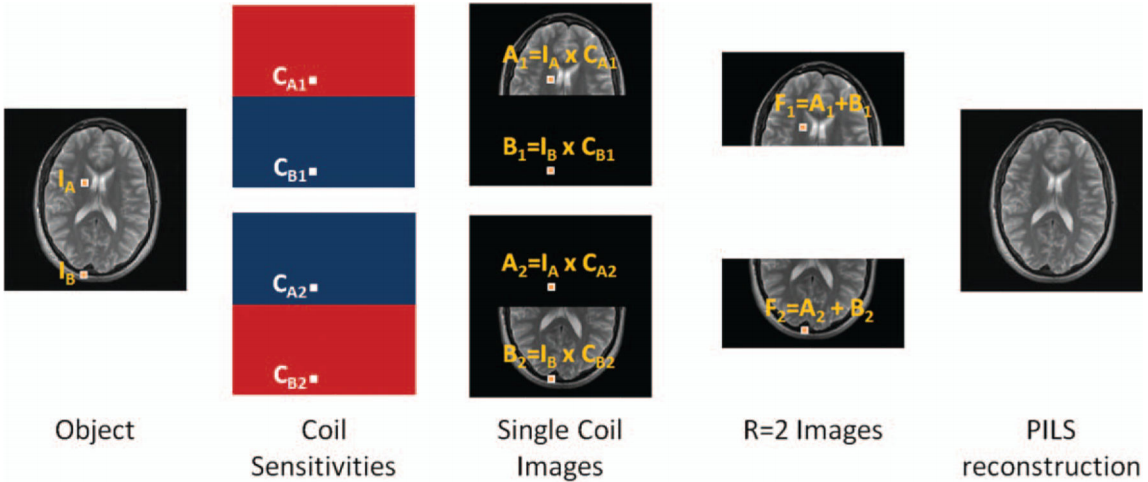
\includegraphics[width=\textwidth,keepaspectratio]{pils}
    \caption{An example of a parallel imaging technique performed with a 2 channel array where the coils have non-overlapping sensitivity profiles. Figure courtesy of \cite{Deshmane2012}}
    \label{fig:pils}
\end{figure}

Obviously, in practical terms this is not feasible. Coil sensitivities will overlap and an algorithm like PILS will fail to reconstruct the image. A more powerful algorithm which unfolds the aliased images, reconstructs a full FOV final image, uses overlapping sensitivity profiles and is actually widely used clinically called SENSE will be the subject of our discussion in the following subsection.

%%%%%%%%%%%%%
\subsection{SENSE Reconstruction} \label{sect:senserec}
Sensitivity Encoding for Fast MRI, or SENSE, is a parallel imaging reconstruction algorithm which is widely used in the clinics. It relies on knowledge of the sensitivity profiles of the individual coils which are used to receive the signal. In practice, the coil maps are calculated at the beginning of a sequence during a prescan. This section is concerned with the main concepts that form the basis for SENSE reconstructions. Although not without problems, mainly caused by patient movement during scan time, SENSE is one of the most popular algorithms used in clinics today. 

As we have discussed before, all parallel imaging techniques have a few things in common. First, undersampled k-space data is acquired and this results in aliased images. If an acceleration factor $R = 2$ is used, then the folding that occurs will translate into 2 pixels being on top of each other. An example of how this might look for 4 channels is presented in Figure~\ref{fig:sense}.

\begin{figure}[ht]
    \centering
    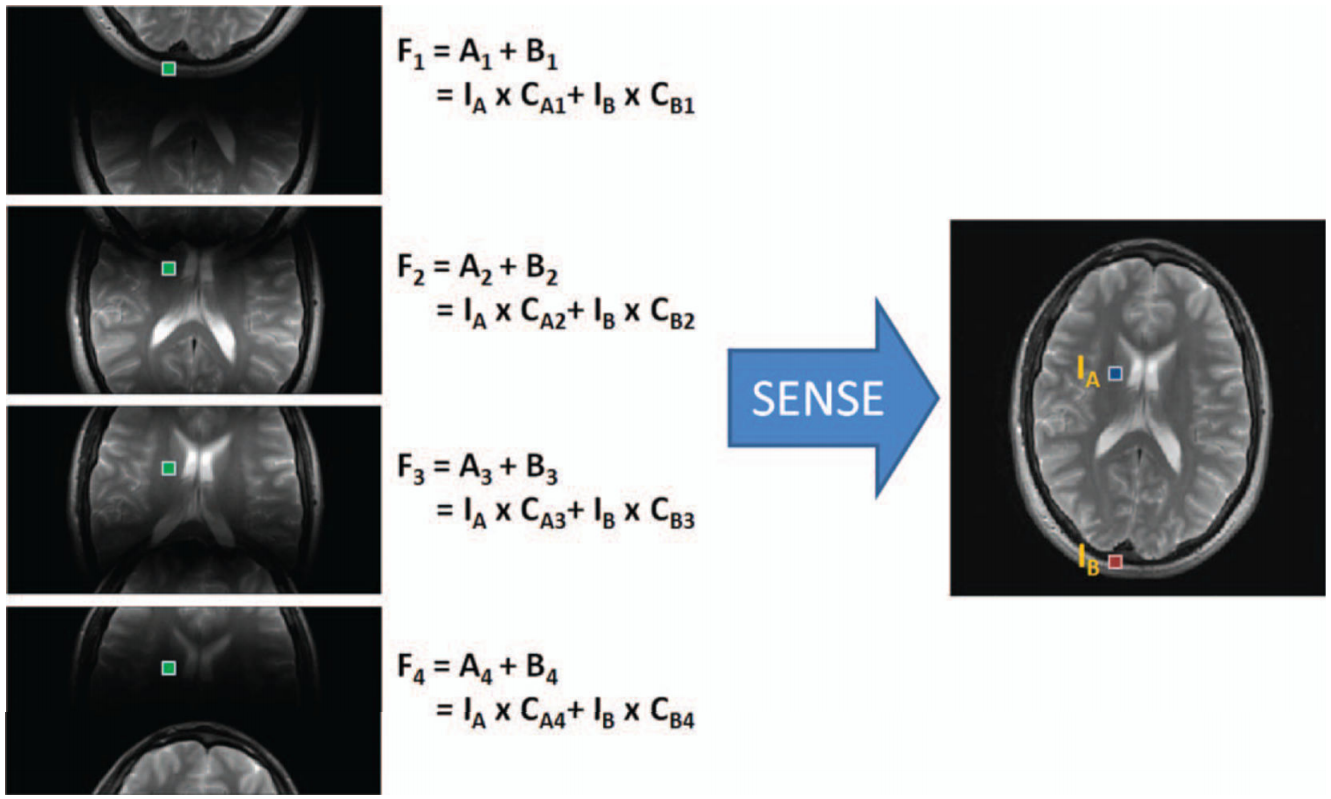
\includegraphics[width=1\textwidth,keepaspectratio]{sense}
    \caption{A 4 channel array SENSE reconstruction for an acceleration factor $R = 2$ is shown here as example. Figure courtesy of \cite{Deshmane2012}}
    \label{fig:sense}
\end{figure}

As mentioned before, SENSE relies on the sensitivity profiles of the coils. It uses this information and the aliased images to 'unfold' the image. This works because, as can be seen in Figure~\ref{fig:sense} where $R = 2$, every voxel intensity is a juxtaposition of 2 intensity values that are coming from the 2 spatial locations which are now on top of each other. So, for example, at the coordinate shown in the first image from the figure, the intensity from the aliased image is just the sum of intensities of those 2 spatial locations ($A_1$ and $B_1$). Moreover, these two locations are actually, as was shown in Figure~\ref{fig:onecoilsens}, directly related to the sensitivity value of the coil at that position. Now, using the same approach for all voxels found at the same spatial coordinate in all images and using the coil sensitivity profiles, we form a linear system that can be solved mathematically.

In our example, the four equations (one for each coil) are:

\begin{flalign*}
    F_1 & = A_1 + B_1 = I_A \times C_{A1} + I_B \times C_{B1} \\
    F_2 & = A_2 + B_2 = I_A \times C_{A2} + I_B \times C_{B2} \\
    F_3 & = A_3 + B_3 = I_A \times C_{A3} + I_B \times C_{B3} \\
    F_4 & = A_4 + B_4 = I_A \times C_{A4} + I_B \times C_{B4} 
\end{flalign*}

which, in matrix form is:

\begin{flalign*}
    \left[
    \begin{array}{c}
        F_1 \\
        F_2 \\
        F_3 \\
        F_4
    \end{array}
    \right]
    = 
    \left[
    \begin{array}{c c }
        C_{A1} & C_{B1} \\
        C_{A2} & C_{B2} \\
        C_{A3} & C_{B3} \\
        C_{A4} & C_{B4} 
    \end{array}
    \right] 
    \times
    \left[
    \begin{array}{c}
        I_A \\
        I_B
    \end{array}
    \right] 
    \Rightarrow
    F = C I
\end{flalign*}

By using Moore-Penrose pseudoinverse, the system of equations can be solved to find the underlying intensity values of the 2 locations, A and B:
\begin{flalign*}
    I = (C^T C)^{-1} C^T F = C^\dagger F
\end{flalign*}
This operation is applied for every spatial location in the image.

As can be expected, a few requirements are needed in order to be able to solve the system of equations. First of all, the number of coils has to be higher than the number of pixels which are juxtaposed for the reconstruction to work. Second, independent channels must not fully intersect each others' sensitivity profiles in order to allow for different weightings of the folded signals. Finally, parallel imaging is known to cause lower signal-to-noise ratio (SNR) values than non-parallel imaging methods due to k-space undersampling \cite{Aggarwal2003}\cite{Xu2005} and coil design \cite{Weiger2001}\cite{Zhu2004}\cite{Ohliger2003}\cite{Lee2004}. The signal-to-noise ratio for SENSE is calculated with the following formula:
\begin{equation}
    SNR_{SENSE} = \frac{SNR_{Original}}{g \sqrt{R}}
\end{equation}
where $g$ is defined as the geometry factor of the coil, or \textit{g-factor} and $SNR_{Original}$ is the signal-to-noise ratio of an MRI image when pMRI is not performed. The "g-factor" describes how good the multichannel receiver array encodes the magnetization distribution of the object \cite{Omer2010}. It is a measure which indicates how much a coil array magnifies the noise at a given location and it is dependent on the number of aliased replicates.

In mathematical terms, the \textit{g-factor} at location $y$ is defined as:
\begin{equation}
    g_y = \sqrt{ [(C^T \Psi^{-1} C )^{-1}]_{yy} (C^T \Psi^{-1} C )_{yy} }
\end{equation}
where $\Psi$ is the noise correlation matrix and $C$ is the sensitivity encoding matrix. This concept is highly used in parallel imaging techniques as it enforces the physical arrangement of the coils used in pMRI scans.

In summary, this section has described the most important concepts behind parallel imaging techniques and reconstructions, with a focus on one of the most popular algorithms, SENSE. The main disadvantage of SENSE reconstruction is the need for accurate coil sensitivity profiles. In addition, motion can be a determining factor when it comes to image quality. Despite these difficulties, SENSE is widely used clinically in order to accelerate MRI scans.






\chapter{MRI Simulation}
\label{chapterlabel3}

Magnetic Resonance Imaging is an imaging technique that is widely used today in clinics and medical research facilities to aid the understanding of how the human body works. It has many applications in the biomedical sciences such as the study of the human anatomy, pathology and even function. 

In contrast to other well established imaging modalities, MRI is incredibly versatile as it is capable of displaying high quality images of any orientation through the human body without the need for the patient to be uncomfortable or move. Furthermore, MRI is based on non-ionizing radiation and it is classified as a non-invasive modality achieving great soft tissue resolution. Its applications span from neuroimaging, heart imaging, angiography, to spectroscopy, diffusion, perfusion imaging, and many others.

The entire process of an MRI scan, from proton to picture, is incredibly complex and requires a great understanding of the underlying physics. Nevertheless, from a high level perspective, a clinical examination using an MR scanner is made up of a few important steps. First, the object that is being imaged and which consists of billions of protons randomly oriented inside the tissue is needed. This object can be an MRI phantom, a tissue sample or an organ of interest. Second, the actual hardware of the MRI scanner is needed in order to create the strong magnetic field used to orient the spins magnetic moments. In addition, gradient coils are needed in order to spatially resolve the spins positions. Also, radio frequency coils are used to transmit rf pulses and to receive the signal generated by the sample. Third, a recipe for how to use the scanner in order to acquire images of desired contrast is needed. Parameters such as RF flip angle, the repetition time and the echo time can be set by the clinician. 

These three main building blocks are necessary in order to produce the signal. Once the signal is generated, it can be collected and sampled in order to be stored in a matrix form, called k-space. When the whole of k-space has been covered, the reconstruction process (a 2D Fast Fourier transform is applied) can start and the final image is obtained. This pipeline is visually presented in Figure~\ref{fig:mriscan}. 

\begin{figure}[H]
    \centering
    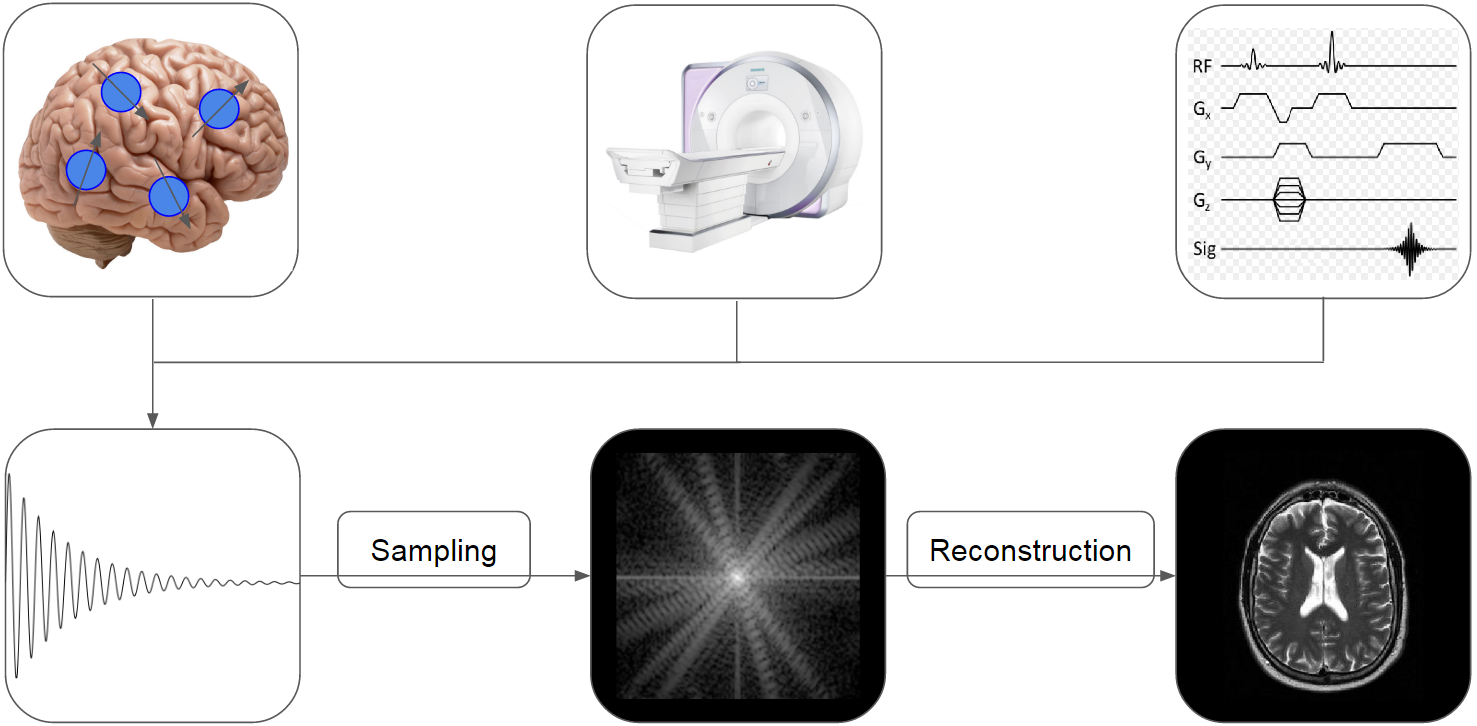
\includegraphics[width=1\textwidth,keepaspectratio]{mriscan}
    \caption{The MRI scan pipeline}
    \label{fig:mriscan}
\end{figure}

However, it is not the full story. A high quality image cannot be achieved unless a few criteria are met. First, the object being imaged has to be completely stationary or motion artefacts will appear in the final image. Even if the patient manages not to move, there is always some movement caused by pulsatile flow or respiration. Second, the scanner's electronic components have an inherent level of noise which will appear in the images. Third, air-tissue boundaries create inhomogeneities in the main magnetic field which will cause distortions in the final images. Fourth, good contrast between the tissue types that are being imaged is achieved when the right combination of sequence parameters is found. All in all, these are just a few of the problems that lead to imperfect images and therefore MRI images need to be corrected and MR parameters need to be mingled with in order to have the best results. 

Under these circumstances, 
the need for MRI simulation was born. There are at least three main reasons for creating an accurate and realistic MR simulator and they can be summarised as follows. First, MR physicists and clinicians need to learn how to use the scanner in order to gain experience. By using an actual MR scanner they would also need a patient or a good phantom to be able to learn how to program a sequence. Moreover, trying out new sequences could take time and scanners are precious medical devices that are needed by patients throughout the year. Second, there is always place for improvement when it comes to contrast-to-noise ratio in MR images. For example, enhancing a pathology in an image requires a fine tuning of the sequence parameters and this process is too time consuming for it to be practiced on a real person and a real MR scanner. Third, there is a large body of research concerning the correction of different imaging artefacts that appear in MR images. All these algorithms require ground truth to be tested and validated against. An MRI simulator can provide this ground truth. In conclusion, simulating the MRI process from object to final image is important and needed in the biomedical sciences.

That being said, the following subsections will be focused on how the ideal simulator should look, what approaches different MRI simulators have taken up until today and how they fit inside the ideal picture and, finally, a review of the active simulators will be provided.

%%%%%%%%%%%%%%%%%%%%%%%%%%
\section{Ideal Simulator}
We have discussed so far about the importance of MRI and the benefits of having an MRI simulator. In this subsection the focus will be on an ideal MRI simulator. As can be expected with any type of physics oriented simulation, the best approach is to emulate the reality as close as possible. That being said, the pipeline presented before is changed to accommodate simulated objects, simulated hardware and simulated sequences. This can be seen in Figure~\ref{fig:mrisimscan}. Now, instead of a real object, we have tissue samples, description of motion patterns and tissue specific parameters. Also, instead of a scanner, we have the scanner specifications being simulated as close to reality as possible and, instead of a real sequence, the sequence specifications are provided and simulated.

\begin{figure}[H]
    \centering
    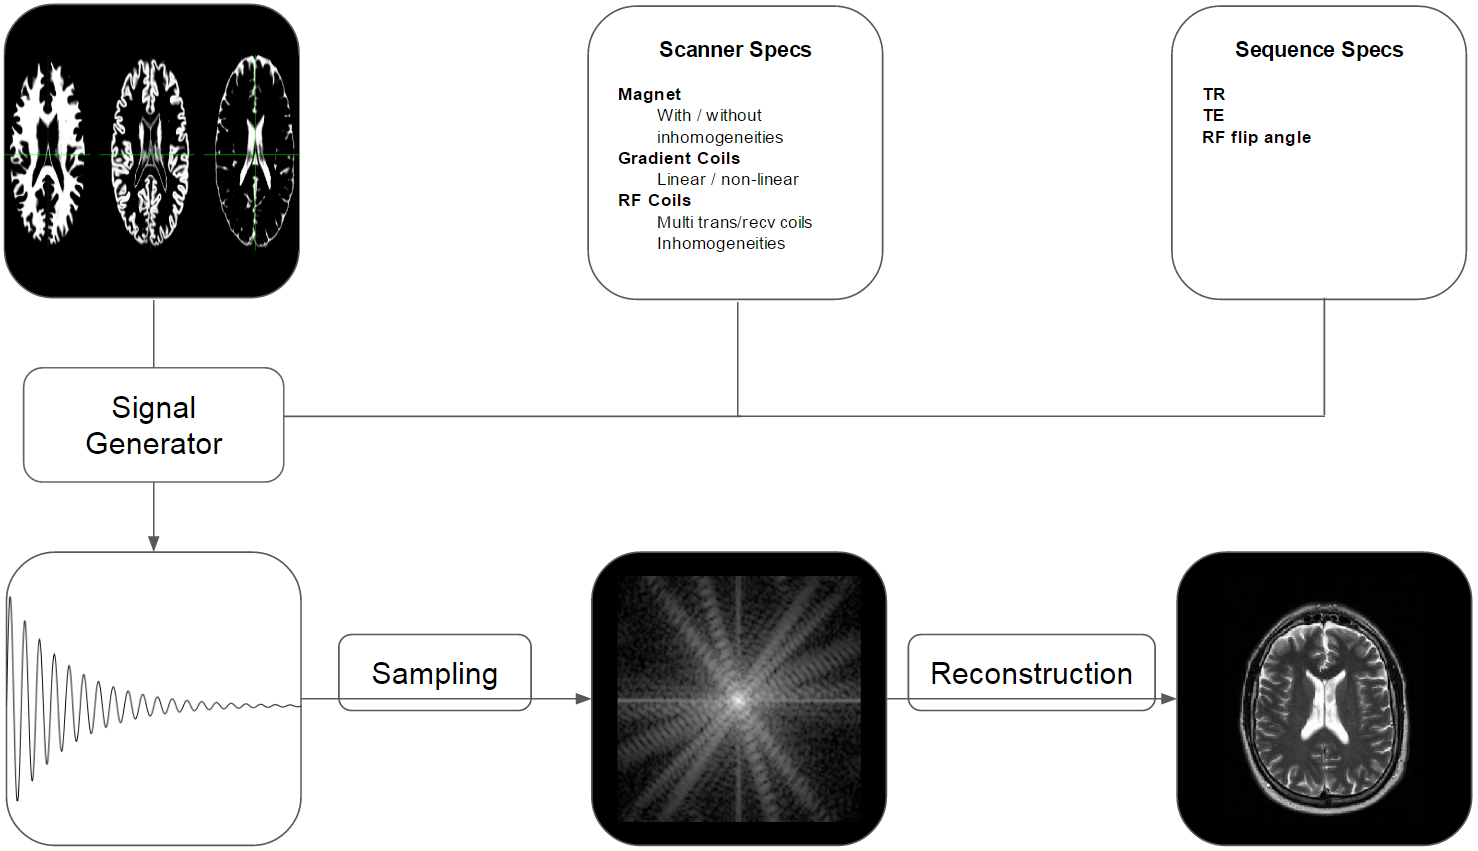
\includegraphics[width=1\textwidth,keepaspectratio]{mrisimscan}
    \caption{The MRI simulation pipeline}
    \label{fig:mrisimscan}
\end{figure}

As can be seen from Figure~\ref{fig:mrisimscan}, a new step was added for the signal creation. Without actual motion from precessing spins, the requirement now is to have a mathematical model that emulates that. Generally speaking, the \textit{Signal Generator} is a Bloch equation solver. 

It follows that, in order to develop a realistic MRI simulator a few criteria must be met. These requirements can be organized in the next categories:

% The next step is to create a taxonomy for the ideal MRI simulator. That being said, the main criteria and their divisions are: \\

\begin{itemize}
%%%% SAMPLE
\item{Sample}

\begin{enumerate}
    %% Geometry
    \item Geometric Representation
    % \begin{itemize}
    %     \item Shape
    %     \begin{itemize}
    %         \item Parametric form
    %         \item Non-parametric form
    %         \begin{itemize}
    %             \item Piecewise constant representation
    %             \item Lattice
    %         \end{itemize}
    %     \end{itemize}
        
    %     \item Resolution
        
    %     \item Relative positions of figures
    %     \begin{itemize}
    %         \item Euclidean representation
    %         \item Graph representation
    %     \end{itemize}
        
    % \end{itemize}
    
    %% Tissue Specific Parameters
    \item Tissue Specific Parameters
    % \begin{itemize}
    %     \item Proton Density
    %     \item $T_1$
    %     \item $T_2$
    %     \item $T_2^*$
    %     \item Chemical Shift
    %     \item Exchange Rates
    %     \item Susceptibility values
    % \end{itemize}
    
    %% Motion
    \item Motion
    % \begin{itemize}
    %     \item Rigid motion
    %     \item Non-rigid motion
    % \end{itemize}
\end{enumerate}


%%%% HARDWARE
\item{Hardware}
\begin{enumerate}
    %% Magnet
    \item Magnet
    % \begin{itemize}
    %     \item Strength
    %     \item Intrinsic inhomogeneities
    % \end{itemize}
    
    %% Gradients
    \item Gradient Coils
    % \begin{itemize}
    %     \item Slew Rates
    %     \item Gradient non-linearities
    % \end{itemize}
    
    %% RF Coils
    \item RF Coils
    % \begin{itemize}
    %     \item Type
    %     \item Number of Coils
    %     \item Intrinsic inhomogeneities
    % \end{itemize}
\end{enumerate}


%%%% SEQUENCE
\item{Sequence}
\begin{enumerate}
    \item Time constants
    % \begin{itemize}
    %     \item TR
    %     \item TE
    %     \item Gradients durations
    %     \item In-between gradients durations
    % \end{itemize}
    
    \item RF Pulse 
    % \begin{itemize}
    %     \item Shape
    %     \begin{itemize}
    %         \item Amplitude
    %         \item Carrier Frequency
    %         \item Initial Phase
    %     \end{itemize}
        
    %     \item Flip Angle
    % \end{itemize}
    
\end{enumerate}

%%%% SIGNAL GENERATOR
% \textbf{4. Signal Generator}
% \begin{itemize}
%     \item Solver
    
%     \item 
% \end{itemize}

%%%% RECONSTRUCTION
\item{Reconstruction}
% \begin{itemize}
    % \item By number of coils
    % \begin{itemize}
    %     \item Single Coil reconstruction
    %     \item Parallel Imaging reconstruction
    % \end{itemize}
% \end{itemize}

%%%% IMPLEMENTATION
% \item{Software Implementation}
\end{itemize}

Next, a survey of existing MRI simulators is being presented in terms of the previously stated criteria.

%%%%%%%%%%%%%%%%%%%%%%%%%%
\section{A survey of MRI Simulators}
%\textbf{Go in depth and explain how every simulator fits in the picture} \\

%%%%%%%%%%%%%%%%%%%
\subsection{Sample}
\subsubsection{Geometric Representation}

Real world objects can have different shapes and sizes. The question now is how these objects are represented geometrically. A first category that can be distinguished is related to how the shape of an object is defined digitally. That being said, the most commonly opted form is the \textit{piecewise constant representation}. This is because storing data in a structured, non-changing shape, where every position in the object is clearly defined and every neighbour is quickly found, is much more convenient for time requirements. 

Indeed, having defined a multi-dimensional matrix with each index representing a position in the object, the search and retrieval of information from the structure is faster than in a linked-list type of structure such as a mesh. Since the first realistic MR imaging simulators developed by Bittoun et al in 1984 \cite{Bittoun1984} who solved the Bloch equation for each point in a 1D object, followed by Summers et al \cite{Summers1986} and by Olsson et al \cite{Olsson1995} who went further, to 3D objects, this has become a standard for all simulators since. 

A different approach was taken by Kwan et al \cite{Kwan1999} who used tissue templates instead of finely grained collections of object points. This helped with computational speed as the magnetization vector was calculated only for the tissue types considered (such as WM, GM and CSF). The object of interest is still divided into cuboid elements and it contains the proportion of each tissue type present. The magnetization for a given voxel is then obtained by weighting the overall magnetization with the proportion of a certain tissue type and then summed over all templates. Although fast, it has many limitations such as the fact that it is not able to simulate certain artifacts caused by different object voxels experiencing different magnetic field inhomogeneities.

\subsubsection{Tissue Specific Parameters}
In terms of tissue specific parameters, ideally, an MRI simulator would have knowledge of every quantifiable element within the real tissue that is of interest to NMR. 

Generally speaking, the contrast in MR images is given by the proton density in that voxel and the tissue relaxation parameters, $T_1$ and $T_2$. That being said, most simulators to date rely on at least these 3 specifications. Bittoun et al \cite{Bittoun1984}, Olsson et al \cite{Olsson1995}, Petterson et al \cite{Petersson1993}, Hacklander et al \cite{Hacklander2005}, Kwan et al \cite{Kwan1999}, Benoit-Cattin et al \cite{Benoit-Cattin2005}, Xanthis et al \cite{Xanthis2014} and Jochimsen et al \cite{Jochimsen2004} require knowledge of PD, $T_1$ and $T_2$. Some other simulators such as the one developed by Drobnjak et al \cite{Drobnjak2006} use $T_2^*$ values instead of $T_2$ as their main focus is on functional MRI which takes into account the local magnetic field inhomogeneities. Others, such as the one created by Stocker et al \cite{Stocker2010} uses knowledge of both $T_2$ and $T_2^*$.

Another interesting aspect of the object being imaged is that of chemical shift as it produces inhomogeneities in the main magnetic field. This is a very important source of imaging artifacts and it is therefore a desired feature in a realistic simulator. Kwan et al \cite{Kwan1999}, Benoit-Cattin et al \cite{Benoit-Cattin2005}, Drobnjak et al \cite{Drobnjak2006}, Stocker et al \cite{Stocker2010}, Xanthis et al \cite{Xanthis2014}, Yoder et al \cite{Yoder2004} and Liu et al \cite{Liu2013} incorporate a $B_0$ inhomogeneity in their simulations.

In addition to these, for more sophisticated simulations, such as those required in \textit{magnetization transfer imaging}, knowledge of the various pools of spins is needed. Such an approach is presented by Liu et al \cite{Liu2016}. 

\subsubsection{Motion}
MRI is a very powerful imaging technique that provides great contrast between soft tissue types. Although one of the most used imaging modalities today, it is known to be prone to motion artifacts. Indeed, the quality of its images is affected by patient movements and pulsatile motion. For this, an accurate and realistic MRI simulator needs to take this into account. 

Clearly, this is a computationally intensive task as it requires calculations of magnetization vectors for all object voxels at each time point when motion is in place. Although it was not possible to simulate until more powerful computers arrived, it has now become one of the most desired traits in a simulator. Indeed, the still active, very powerful and realistic simulators treat this aspect within their software tool. Petterson et al \cite{Petersson1993} incorporates movement (or flow) in its k-space formalism approach without the possibility of simulating blurring artifacts. More sophisticated approaches such as those developed by Drobnjak et al \cite{Drobnjak2006} and Jochimsen et al \cite{Jochimsen2004} simulate rigid body motion during acquisition.

%%%%%%%%%%%%%%%%%%%
\subsection{Hardware}
\subsubsection{Magnet}
One of the key components of the MR scanner is the main magnet. It is an expensive piece of equipment used to generate the high fields required in MR imaging. Clinically, there are a few types of magnets available: closed bore (most widely used clinically as its strength range starts at 1T), open bore (these are permanent magnets with strengths that range from 0.2T and 0.7T) and dipolar electromagnets configurations (with a range of 0.5T to 1.2T) \cite{Morrow2000}. Regardless of their type, MR imaging requires perfect homogeneity in the field such that every part of the object being scanned experiences the expected field strength. In reality, parallel field lines are hard to obtain and so a scanner is equipped with shim coils which adjust the homogeneity of the field \cite{Romeo1984}.

That being said, a realistic MRI simulator should be equipped with at least 2 specifications: field strength and inhomogeneities in the main magnetic field. As the current aim of many MRI simulators is to provide a realistic, yet controlled way of generating MR images, all simulators available offer the possibility of field strength choice. In terms of intrinsic magnet inhomogeneities, there are no available simulators that model that, most of them focusing on susceptibility induced inhomogeneities as was discussed previously.

\subsubsection{Gradient Coils}
Gradient coils are part of the MR scanner hardware. Their purpose is to linearly vary the main magnetic field in a certain direction. Nearly all clinically available MR scanners have 3 types of gradient coils: the x-, y- and z- gradients, which alter the main magnetic field such that different parts of the object being imaged experience a slightly different field strength \cite{Hidalgo-Tobon2010}. This is at the heart of slice selection and frequency encoding, concepts which were discussed in the previous chapter. 

Turning to MRI simulation, it is obvious that the most important requirements that need to be part of the simulation pipeline are the gradient's strength and its direction. Besides this, other aspects are also essential. For example, one might want to model a non-linear variation in the gradients strength. This is available in the simulators developed by Benoit-Cattin et al \cite{Benoit-Cattin2005}, Stocker et al \cite{Stocker2010} and Liu et al \cite{Liu2013}. In addition, the time it takes for a gradient to reach its peak, called the \textit{rise time}, must be taken into consideration when realistic MRI simulation is desired. The most important reason for this is that the slew rates affect the minimum attainable TR or the spacing between spin echoes in fast imaging sequences. Among the available simulators, Drobnjak et al \cite{Drobnjak2006} and Xanthis et al \cite{Xanthis2014} allow for rise time configuration.

Furthermore, Jochimsen et al \cite{Jochimsen2004} provide a list of rotation matrices that can be used to move the gradient objects for diffusion MRI experiments. These matrices can also be user defined. In addition, Drobnjak et al \cite{Drobnjak2010} simulate time varying magnetic fields which are the main cause for eddy currents artifacts in diffusion MRI. 

\subsubsection{RF Coils}
The third main hardware component of an MR scanner is the RF coil. There are roughly two types of coils: volume and surface coils. The main difference between the two, besides their suggestive usage, is that the surface coils have a lower penetration depth than the volume ones. The surface coils are therefore able to retrieve better SNR for surface originating signals, while the volume coils provide a more homogeneous field. The spatially varying signal strength specific to surface coils is modelled by Stocker et al \cite{Stocker2010} and by Xanthis et al \cite{Xanthis2014} in their MRI simulators.

Now, as with any piece of electronic equipment, the scanner's RF coils are not perfect. It is therefore important when simulating the MRI pipeline to take inhomogeneities into consideration. Hacklander et al \cite{Hacklander2005} and Drobnjak et al \cite{Drobnjak2006} model noise and inhomogeneities in the receiving and transmitting coils. 

Moreover, multiple coils can be used simultaneously to transmit and receive signals. This is an available feature in the simulators developed by Jochimsen et al \cite{Jochimsen2004}, Liu et al \cite{Liu2014} and Stocker et al \cite{Stocker2010}.

%%%%%%%%%%%%%%%%%%%
\subsection{MRI Sequence}
The discussion so far was centered around the object being imaged and the MR scanner hardware. Another important part of the pipeline is the MRI sequence, which can be described as a set of radiofrequency pulses and changing magnetic field gradients, together with the order in which each of them should be performed and for how long. This "recipe" dictates the contrast in the image or the type of information available. For example, there are MRI sequences which can provide good anatomical contrast between different tissue types, while more sophisticated ones can be sensitized to flow or perfusion. Despite their large number, all of them rely on a set of parameters that can be modified in order to provide the best contrast for the requirements. 
%There are two main ways of categorizing the sequences: by the contrast provided (proton density, $T_1$, $T_2$ or $T_2^*$ weighted) or by their type (spin echo, gradient echo, etc).
In this section different MRI simulators will be investigated in terms of how they simulate the MR sequence.

\subsubsection{Time constants}
As stated before, all MRI sequences have a set of time related parameters that ultimately define the image contrast. That being said, one particularly popular approach in terms of simulation is to use the steady state solutions of the Bloch equations for some of the most clinically used sequences. For example, the spin-echo sequence can be described in terms of tissue specific parameters (proton density, $T_1$ and $T_2$) and sequence specific parameters such as: time to echo ($TE$) and time to repetition ($TR$). This approach aids the understanding of MR image contrast when the time constants are modified and is present in MRI simulations developed by Ortendahl et al \cite{Ortendahl1984}, Riederer et al \cite{Riederer1984}, Bobman et al \cite{Bobman1985}, Lufkin et al \cite{Lufkin1986}, Torheim et al \cite{Torheim1994}, Simmons et al \cite{Simmons1996} and Hacklander et al \cite{Hacklander2005}. 

Spin echo is not the only sequence that can be simulated this way. By adding a different time constant, the inversion time ($TI$), inversion-recovery sequences can be modelled. These are simulated by Ortendahl et al \cite{Ortendahl1984}, Torheim et al \cite{Torheim1994}, Simmons et al \cite{Simmons1996} and Torheim et al \cite{Torheim1994}. More sophisticated sequences such as saturation recovery or fast sequences such as FLASH or turbo spin echo, which require a flip angle smaller than $90^o$, are also modelled by Simmons et al \cite{Simmons1996} and Hacklander et al \cite{Hacklander2005}.

Turning to simulators which solve the Bloch equation for each object voxel and for each time point during the sequence, the time constants are generally the same. That being said, $TE$, $TR$ and $\alpha$ (flip angle) can be chosen in simulators developed by Benoit-Cattin et al \cite{Benoit-Cattin2005}, Stocker et al \cite{Stocker2010}, Drobnjak et al \cite{Drobnjak2006} and Kwan et al \cite{Kwan1999}. Moreover, predefined gradient echo and spin echo sequences are offer by Benoit-Cattin et al \cite{Benoit-Cattin2005} and Drobnjak et al \cite{Drobnjak2006}, while Jochimsen et al \cite{Jochimsen2004} offer, in addition, predefined PROPELLER-EPI, single-shot TrueFISP, multi-slice MDEFT and fully flow-compensated FLASH sequences.

Finally, Drobnjak et al \cite{Drobnjak2006} and Xanthis et al \cite{Xanthis2014} allow users to define their own pulse sequences. These take the form of an input file which contains the sequence parameters ($TE$, $TR$, field-of-view, flip angle, gradient strengths, etc) in a simulator dependent structure. Jochimsen et al \cite{Jochimsen2004} treats the pulse sequence creation from a object-oriented perspective, providing a class structure that can be easily extended with new functionality.

\subsubsection{RF Pulse}
RF pulses are an important part of the MRI scanning pipeline. They are key to image formation as they "tip" the net magnetization vector away from the main magnetic field allowing it to be eventually measured, sampled, stored into k-space and finally reconstructed into an image. Moreover, the carrier frequency of the RF pulses has to be equal to the Larmor frequency of the spins which reside in the slice of interest. This is one of the key components of slice selection.

It is therefore important to accurately simulate this behaviour. Although most simulators treat the RF pulse as an event which rotates the net magnetization vector through a flip angle, simulators developed by Xanthis et al \cite{Xanthis2014}, Jochimsen et al \cite{Jochimsen2004} and Liu et al \cite{Liu2013} offer different types of RF pulse models to be investigated. Among all, the common ones are: slice selective RF pulses (sinc and Gauss shaped), rectangular and adiabatic. Moreover, composite pulses, created by concatenating other available pulses, are offered by ODIN, the simulator developed by Jochimsen et al \cite{Jochimsen2004}.

%%%%%%%%%%%%%%%%%%%
\subsection{Reconstruction}
The steps described thus far included the object, the scanner hardware and the process of obtaining different types of contrasts in the final MR images. Next, signal arising from the excited tissue is collected during read out, sampled and then stored in a matrix form. The matrix form represents the image in the frequency domain and it is known as k-space. Performing an inverse Fourier transform allows the normal image to be reconstructed.

However, almost all clinical MRI scanners have recently incorporated more sophisticated reconstruction methods. One of these methods sits under the \textit{parallel imaging techniques} umbrella. These are a collection of reconstruction algorithms that can be used in conjunction with many existing imaging sequences to speed up scanning time. This can be achieved by skipping time-consuming phase-encoding steps and replacing the missing information with data coming from multiple receiver coils. 

Therefore, in order to achieve parallel imaging, two criteria must be met. First, instead of using one homogeneous volume coil, multiple rf surface coils distributed around the object of interest will be used. Each of these coils will have a particular sensitivity profile which is used to recover the missing information caused by skipping phase-encoding steps. Second, a reconstruction algorithm will reconstruct the final, unaliased, image by using the undersampled data and the individual coil sensitivities. 

Generally speaking, there are two types of reconstruction algorithms: the \textit{GRAPPA\footnote{GeneRalized Auto-calibrating Partially Parallel
Acquisition}-type} algorithms, which use the k-space undersampled data to reconstruct the images and the \textit{SENSE\footnote{SENSitivity Encoding}-type} algorithms, which use the aliased images to reconstruct the final artifact free images \cite{Deshmane2012}. There are also hybrid algorithms such as ASSET\footnote{Array Spatial Sensitivity Encoding Technique} and ARC\footnote{Auto-calibrating Reconstruction for Cartesian
Imaging}, both being implemented by GE\footnote{General Electric} scanners \cite{Yanasak2015}.

That being said, parallel imaging techniques should be addressed in simulation in order to develop new algorithms or to test the validity of the already existing ones. Moreover, besides being more cost effective than normal scans, pMRI can increase motion tolerance \cite{Yanasak2014}, making it a highly desirable feature. Although the simulators developed by Stocker et al \cite{Stocker2010}, Liu et al \cite{Liu2013} and Jochimsen et al \cite{Jochimsen2004} have multi-coil capabilities, only the latter one implements a pMRI reconstruction algorithm, more specifically, GRAPPA.

%%%%%%%%%%%%%%%%%%%%%%%%%%
\section{Active MRI Simulators}
This section will be concerned with the active MRI simulators. A description of each will be provided with the focus being on the most desirable features. In doing so, the key players will be identified and the MRI simulation stage will be set.

To begin with, patient movement is the most common cause for imaging artifacts. More often than not it is caused by involuntary actions such as blood flow, respiration or cardiac pulse, but it can also be caused by external factors such as mechanical vibrations. The resulting artifacts are called \textit{blurring} and \textit{ghosting} and are the result of phase and amplitude incongruities \cite{Pusey1986} between consecutive phase encoding steps. That being said, simulating motion artifacts is one of the most highly desirable MRI simulation features. Out of all active simulators, three of them simulate rigid-body motion during acquisition. These simulators are called POSSUM\footnote{Physics-Oriented Simulated Scanner for Understanding MRI} \cite{Drobnjak2006}, JEMRIS \cite{Stocker2010} and MRiLab \cite{Liu2013}.

Second, multicoil acquisition has become a standard in clinical MRI scanners as it is the first step towards faster scans when used in conjunction with parallel imaging reconstruction algorithms. That being said, it is an important feature to have in an MRI simulator. Of all active players, JEMRIS \cite{Stocker2010}, MRiLab \cite{Liu2013} and ODIN \cite{Jochimsen2004} provide multicoil acquisitions. Moreover, MRiLab \cite{Liu2013} offers the possibility to graphically construct the coil configuration or to load a user defined one.

Third, as MRI simulation is highly expensive computationally, most available simulators perform their experiments on cluster systems to reduce run time. In case one does not have a readily available cluster, a couple of the active simulators offer an alternative: GPU\footnote{Graphics processing unit} implementation. This is a more user friendly approach as GPUs are known to be highly powerful processing units and are most often than not available on personal computers. The MRI simulators which have this feature are MRISIMUL \cite{Xanthis2014} and MRiLab \cite{Liu2013}.

Finally, as previously stated, parallel reconstruction is a highly desirable trait. This is because all known MRI scanners clinically available implement one or two pMRI reconstruction algorithms. The only available simulator which performs GRAPPA reconstructions is ODIN \cite{Jochimsen2004}. 

These four described aspects of MRI simulation and the key players which implement them can be visually inspected in Figure~\ref{fig:activesim}, which also sets the stage for currently active MRI simulators.  

\begin{figure}[H]
    \centering
    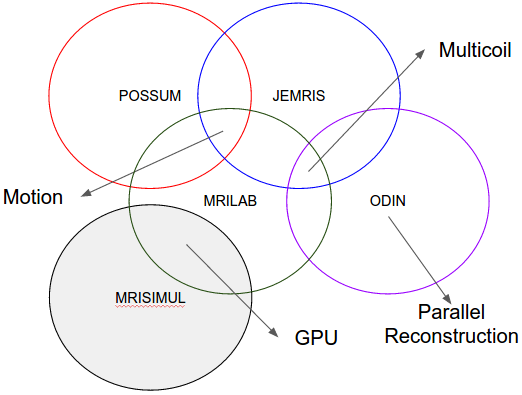
\includegraphics[width=\textwidth,keepaspectratio]{activesim}
    \caption{Active MRI Simulators}
    \label{fig:activesim}
\end{figure}

In conclusion, this section has presented the history of MRI simulation and its most important aspects in terms of a realistic MRI scan. The final subsection was focused on some of the most desirable features an MRI simulator should have. In doing so, it was found that parallel imaging techniques are not currently investigated by many of the aforementioned players. The purpose of this project is therefore to add parallel imaging capabilities to POSSUM, the \textit{Physics Oriented Simulated Scanner Utility for MRI} software tool developed by Drobnjak et al \cite{Drobnjak2006} and part of the FMRIB's software library\footnote{Created by the Analysis Group, FMRIB, Oxford, UK  \url{http://fsl.fmrib.ox.ac.uk/fsl/fslwiki/FSL}}.


\chapter{Simulating Parallel Imaging}
\label{chapterlabel4}

Following on from the last chapter, which discussed existing simulation strategies, this chapter will focus on how parallel imaging was implemented in POSSUM, from generating sensitivity profiles for the coils, to SENSE image reconstruction. This chapter will also describe SENSE in more detail.

%%%%%%%%%%%%%%%%%%%%%%%%%%
\section{Introduction}
The MRI simulation software used in this thesis is called \textit{Physics Oriented Simulated Scanner Utility for MRI}, or \textit{POSSUM}, and it is part of FSL (FMRIB's Software Library) \footnote{Created by the Analysis Group, FMRIB, Oxford, UK  \url{http://fsl.fmrib.ox.ac.uk/fsl/fslwiki/FSL}}. It is a Bloch equation based simulator which consists of several modules that work together in order to produce a realistic MRI image. This process can be seen in Figure~\ref{fig:possumsim}.  

As stated before, the main goal of this simulator is to produce realistic MRI images given a set of input objects. For that reason, in the remaining of this section the focus will be on the inputs to the simulator that were used in our simulations and will describe them in more depth: 

\begin{figure}[H]
    \centering
    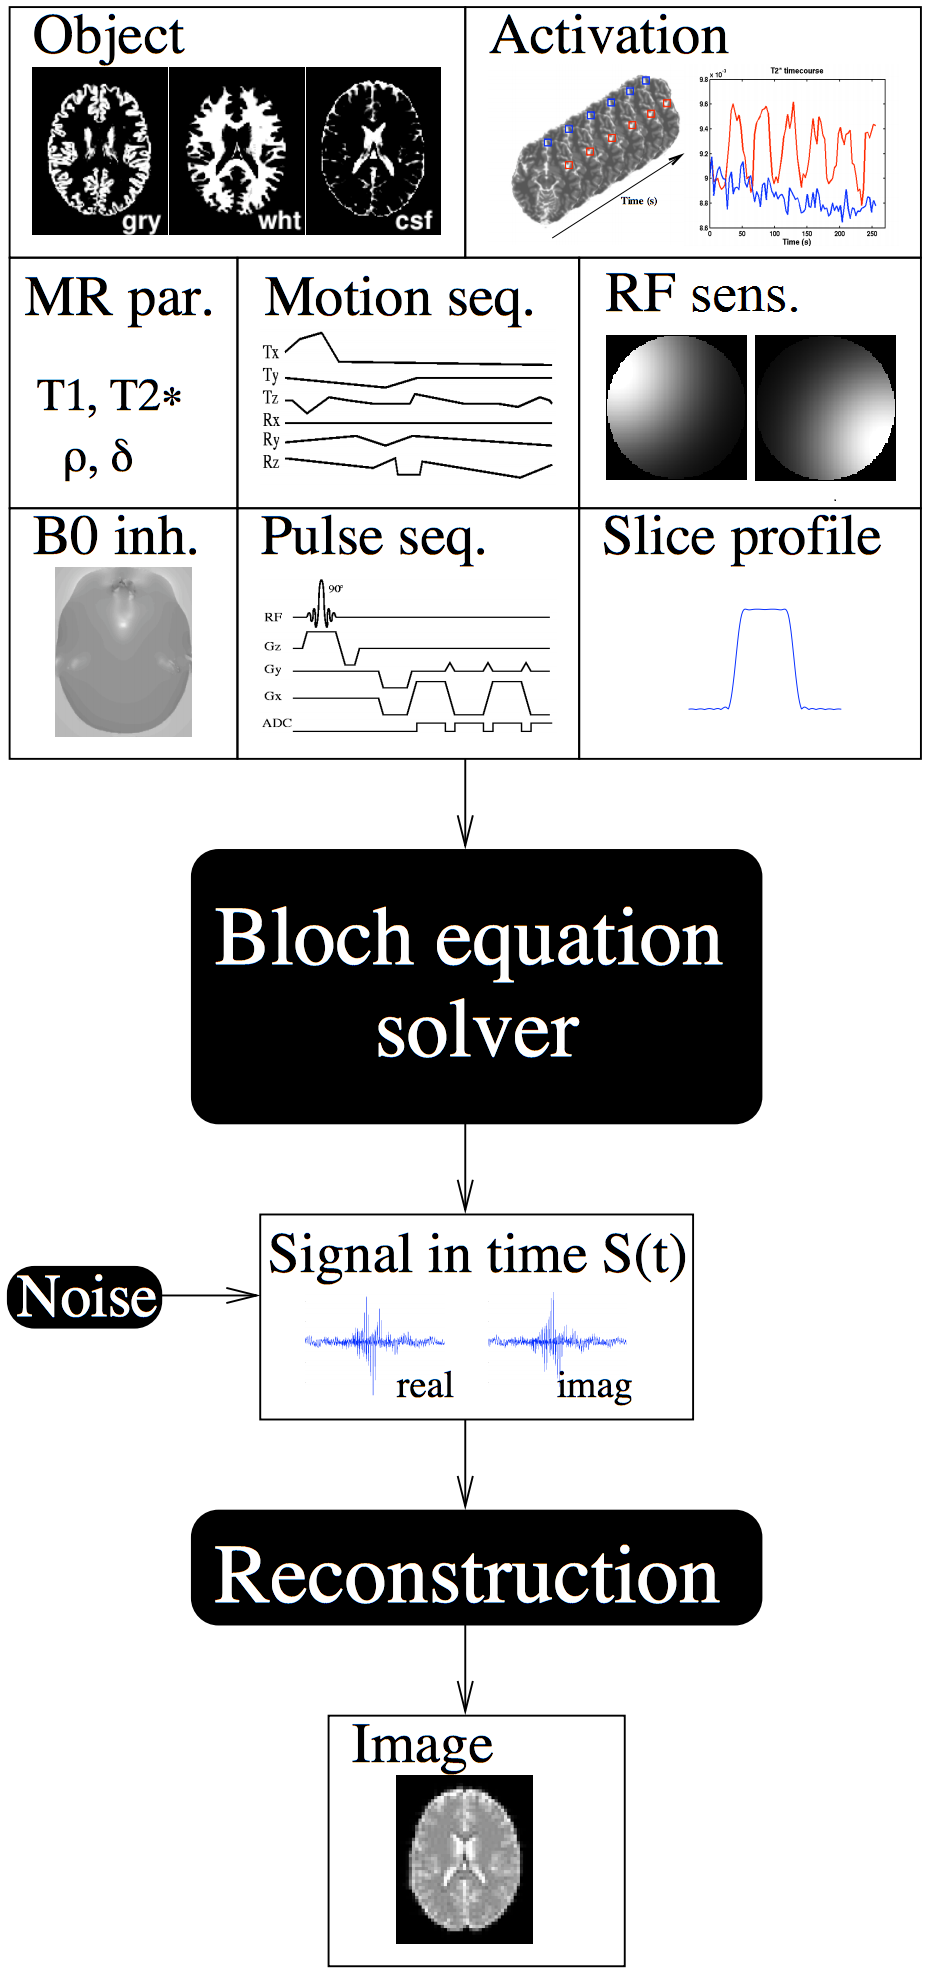
\includegraphics[width=.7\textwidth,keepaspectratio]{possumsim2}
    \caption{POSSUM simulation process in which the Bloch equation solver module receives as input: the object, motion sequence, pulse sequence, $B_0$ inhomogeneities, MR parameters, RF coil sensitivity profiles, slice profile, etc., it produces a signal, adds noise to it and then reconstructs the signal into an image using Fast Fourier Transform (FFT). Figure courtesy of: \cite{Drobnjak07}. Figure was modified to incorporate \textbf{RF coil sensitivity profiles}.}
    \label{fig:possumsim}
\end{figure}

\textit{The object} that POSSUM works with is a four-dimensional anatomical voxel model consisting of different tissue types. For the brain model, 3 tissue types are used: white matter, gray matter, and cerebro-spinal fluid, as seen in Figure~\ref{fig:tissuetemp}. The anatomical models used in POSSUM were produced by the group from McConnell Brain Imaging Centre, Montreal Neurological Institute, McGill University \cite{Kwan1999}, \cite{Cocosco1996}, \cite{Collins1998}. The brain model used in this thesis is made up of 192 x 192 x 192 cuboid voxels of 1mm x 1mm x 1mm in size. Each element contains a value between 0 and 1, representing the proportion of a particular type of tissue in that voxel.

\begin{figure}[H]
    \centering
    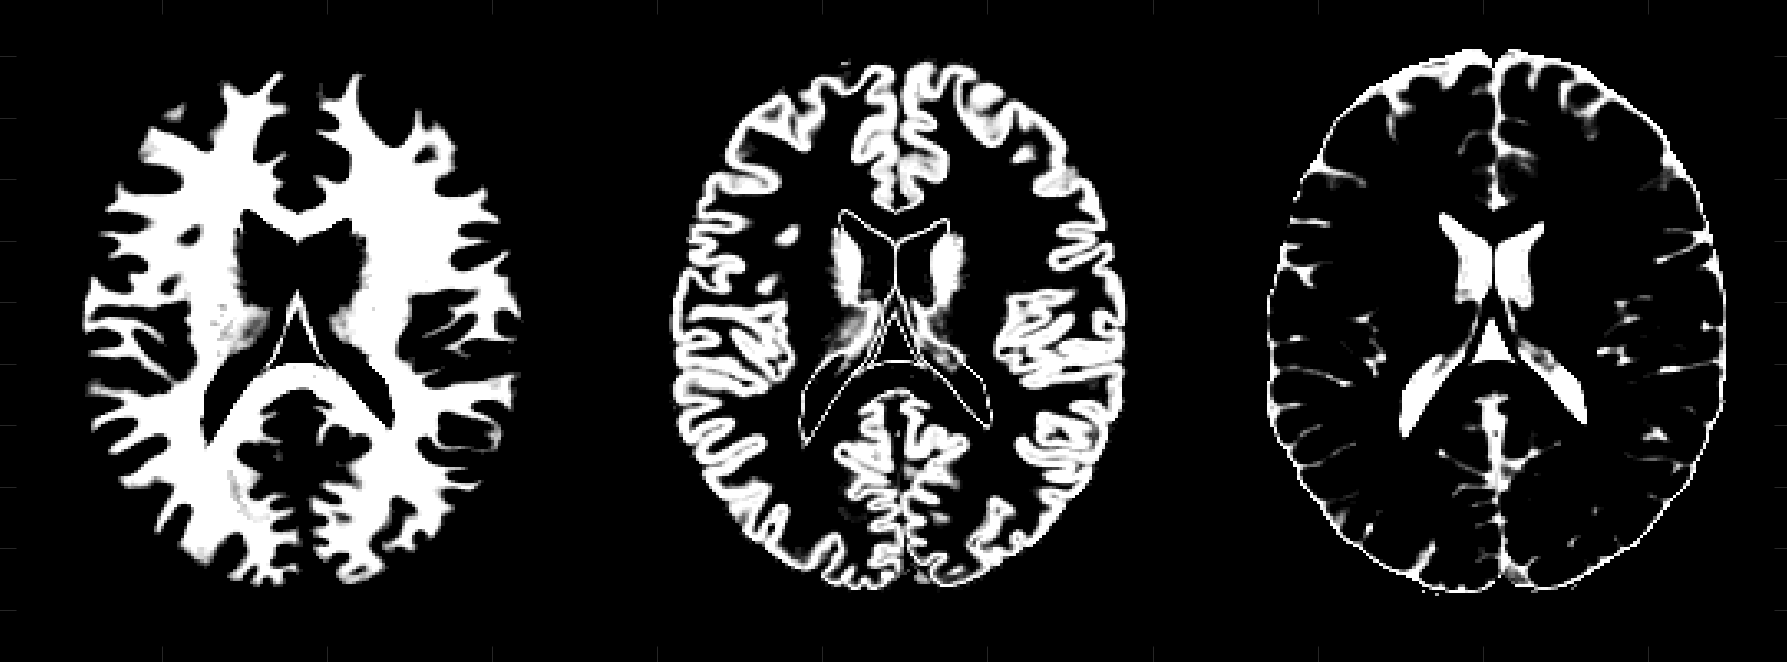
\includegraphics[width=.7\textwidth,keepaspectratio]{tissuetemp}
    \caption{Cross-section tissue templates example showing, from left to right, white matter, gray matter and cerebrospinal fluid}
    \label{fig:tissuetemp}
\end{figure}

\textit{The MR parameters} (relaxation times and spin density $\rho$) for each tissue type in the brain model are offered as input to POSSUM in the form of a matrix. The values for the three tissue types described before were derived by the same group which created the digital brain phantom and can be found in Table~\ref{tab:mrparams}. These values were used throughout all of the simulations from this thesis.

\begin{table}[h!]
\centering
\begin{tabular}{||c c c c ||} 
 \hline
 Tissue Type & $T_1$ (ms) & $T_2^*$ (ms) & $\rho$   \\ [0.5ex] 
 \hline\hline
 Gray Matter & 833 & 83 & 0.86   \\ 
 White Matter  & 500 & 70 & 0.77   \\
 CSF  & 2569 & 329 & 1 \\
 \hline
\end{tabular}
\caption{The MR parameters used in this thesis for different tissue types}
\label{tab:mrparams}
\end{table}

\textit{The pulse sequence} is defined as a series of values in matrix form for the gradients (frequency encoding, phase encoding and slice select), for the RF pulse (angle, frequency bandwidth and frequency centre parameters) and for the signal read-out times. An example of how this table looks like can be seen in Figure~\ref{fig:pulseseqtable}. Also, it is worth mentioning, that the current version of POSSUM simulates two very common pulse sequences, EPI (Echo Planar Imaging) and GE (Gradient Echo), with the possibility to provide a user-defined sequence as well.

\begin{figure}[H]
    \centering
    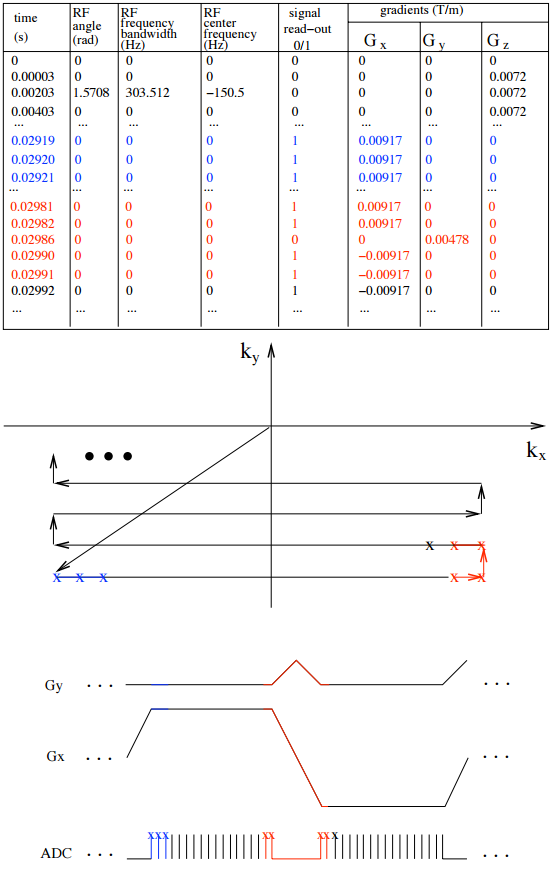
\includegraphics[width=.7\textwidth,keepaspectratio]{pulseseqtable2}
    \caption{The pulse sequence matrix for the POSSUM EPI sequence together with the k-space trajectory. Figure courtesy of \cite{Drobnjak07}}
    \label{fig:pulseseqtable}
\end{figure}

\textit{The motion sequence} can be specified as a file containing values for time (in seconds), for translations ($T_x$, $T_y$ and $T_z$, in meters) and for rotations ($R_x$, $R_y$ and $R_z$, in radians) about the centre of the volume.

\textit{The slice profile} is given in terms of a matrix where the first column specifies the frequency and the second one specifies the amplitude of the RF pulse. The slice profile used in my simulations was derived from a Varian 3T scanner and has a realistic profile which can be viewed in Figure~\ref{fig:sliceprof}. 

\begin{figure}[H]
    \centering
    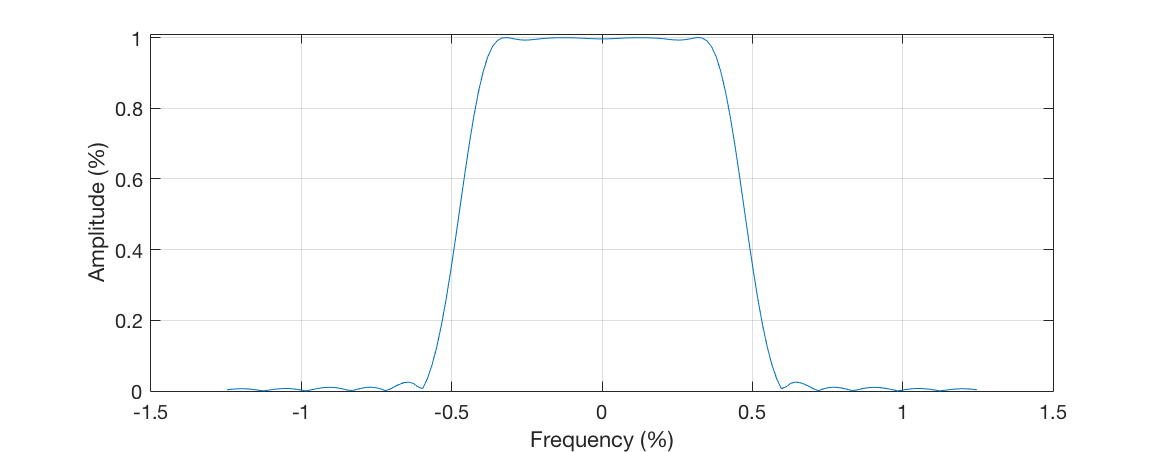
\includegraphics[width=1\textwidth,keepaspectratio]{slcprof}
    \caption{The windowed-sinc RF pulse envelope shape used in POSSUM}
    \label{fig:sliceprof}
\end{figure}

In addition to these input objects, we have created an input object called \textit{coil sensitivity profiles} which will be used for parallel imaging. The next section will cover their implementation and usage in POSSUM.

%%%%%%%%%%%%%%%%%%%%%%%%%%
\section{Coil Sensitivity Profiles}
As has been discussed before, all parallel imaging techniques rely on some knowledge of the multichannel receiver array. Each individual coil from this array has its own sensitivity profile which is dependent on the coil's position with respect to the object being imaged. These maps also show how each individual coil is sensitive to the signal coming from a different spatial location of the desired field of view. As an example, consider an array of 8 coils uniformly distributed in a circle around an object of interest. As shown in Figure~\ref{fig:8coils}, these coils will be sensitive to the signal coming from a limited region of the object.

\begin{figure}[H]
    \centering
    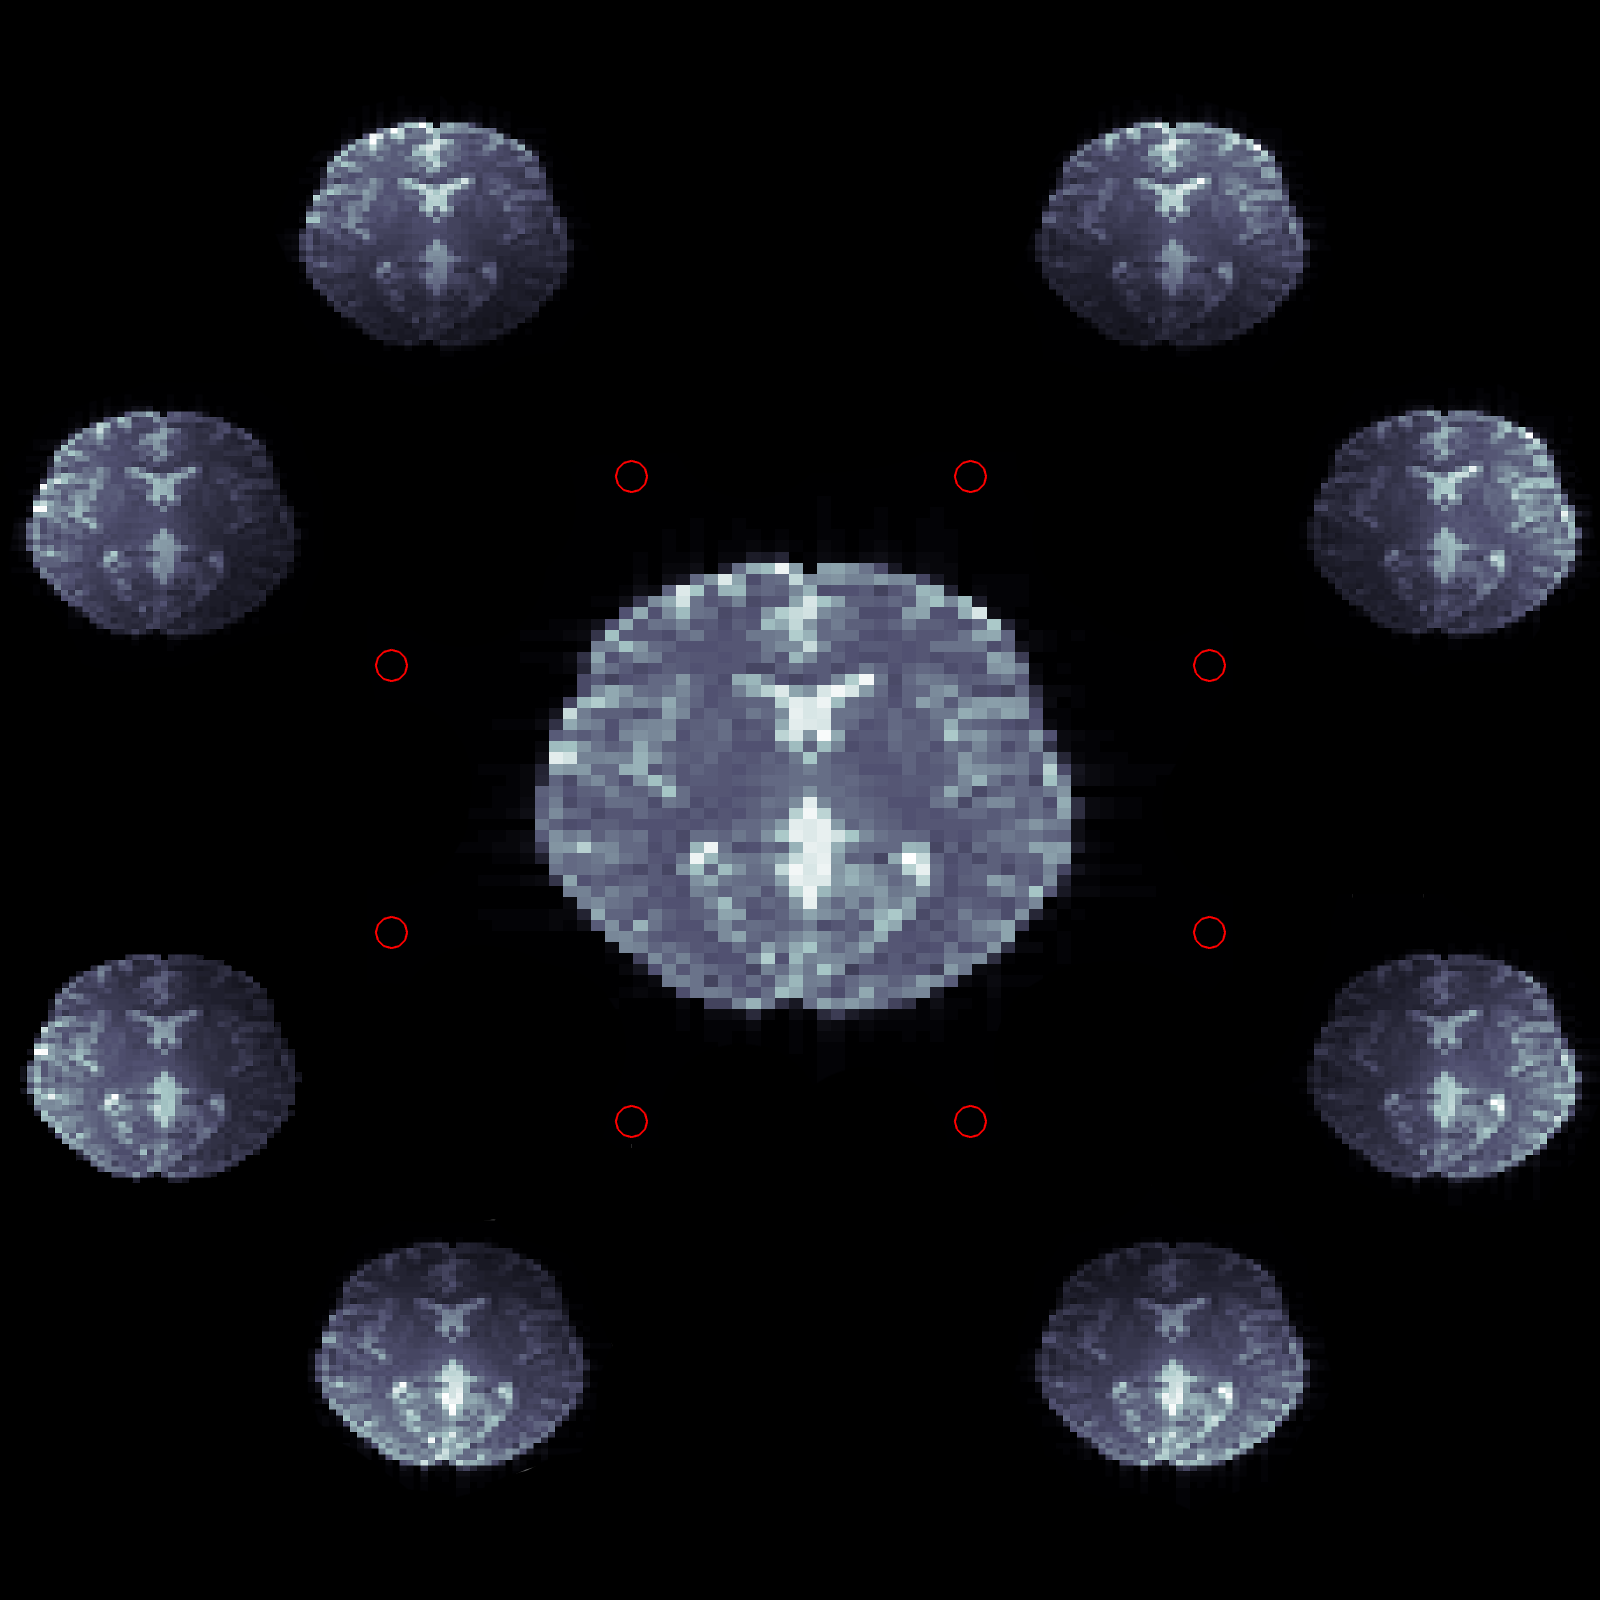
\includegraphics[width=1\textwidth,keepaspectratio]{9brains}
    \caption{An example of a head multichannel receiver array made up of 8 coils. Each red circle is the position of one of the channels}
    \label{fig:8coils}
\end{figure}

In a clinical setting, these coils will be arranged around the object of interest in such a way that each individual coil will cover only part of the FOV and, when put together, they will cover the full FOV. One application that results in increased signal-to-noise ratio \cite{Hayes1991} is to collect the signal from each channel, reconstruct the images and combine them into one final image using a sum-of-squares operation \cite{Roemer1990} or using more sophisticated methods such as those proposed by Walsh et al \cite{Walsh2000}. In addition, great care is taken with how the array is arranged to provide the best possible results, as different body parts have different requirements. For example, a head coil will be arranged in a circular fashion, while a spine array will be linear. Clinically, such arrays can be comprised of 4, 8 and can go up to 32 channels, depending on the application. Each of these coils can have a changing sensitivity in 2 or 3 directions. Since coil sensitivity profiles can provide the extra information missing when parallel imaging is desired, acceleration can occur only in the direction of sensitivity variation. For instance, in case the phased-array coil arrangement is as shown in Figure~\ref{fig:5coils}, parallel imaging will be possible only in the direction of variation between coils, and it will not be possible in the horizontal direction where coil sensitivities do not change \cite{Deshmane2012}. Moreover, in a clinical setting, phased array coils are arranged such that their channels provide maximum variation in the standard phase-encoding directions. 

\begin{figure}[H]
    \centering
    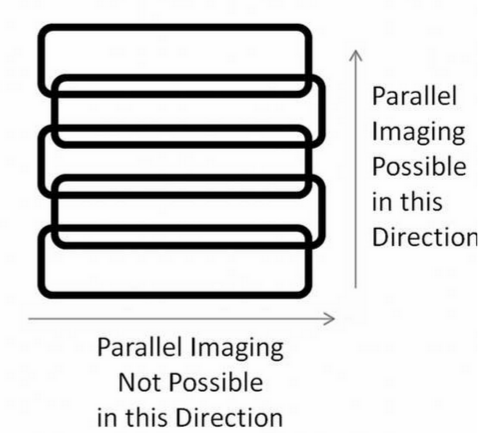
\includegraphics[width=.6\textwidth,keepaspectratio]{5coils}
    \caption{Parallel imaging possible in direction of coil sensitivity variation. Figure courtesy of \cite{Deshmane2012}}
    \label{fig:5coils}
\end{figure}

Turning to an individual coil, it is interesting to investigate more closely how each channel will change the MR image given its intrinsic non-homogeneous sensitivity profile. An example of this can be found in Figure~\ref{fig:1coil} where an object, such as the brain slice found in the left hand side of the figure, is weighted by the sensitivity profile of a given coil (middle image), resulting in the MR image as seen by that channel (right hand side of the figure). Mathematically, this says that each voxel's intensity value from the final image is the result of weighting each voxel's intensity value from the object image by the coil's sensitivity at that location.

\begin{figure}[H]
    \centering
    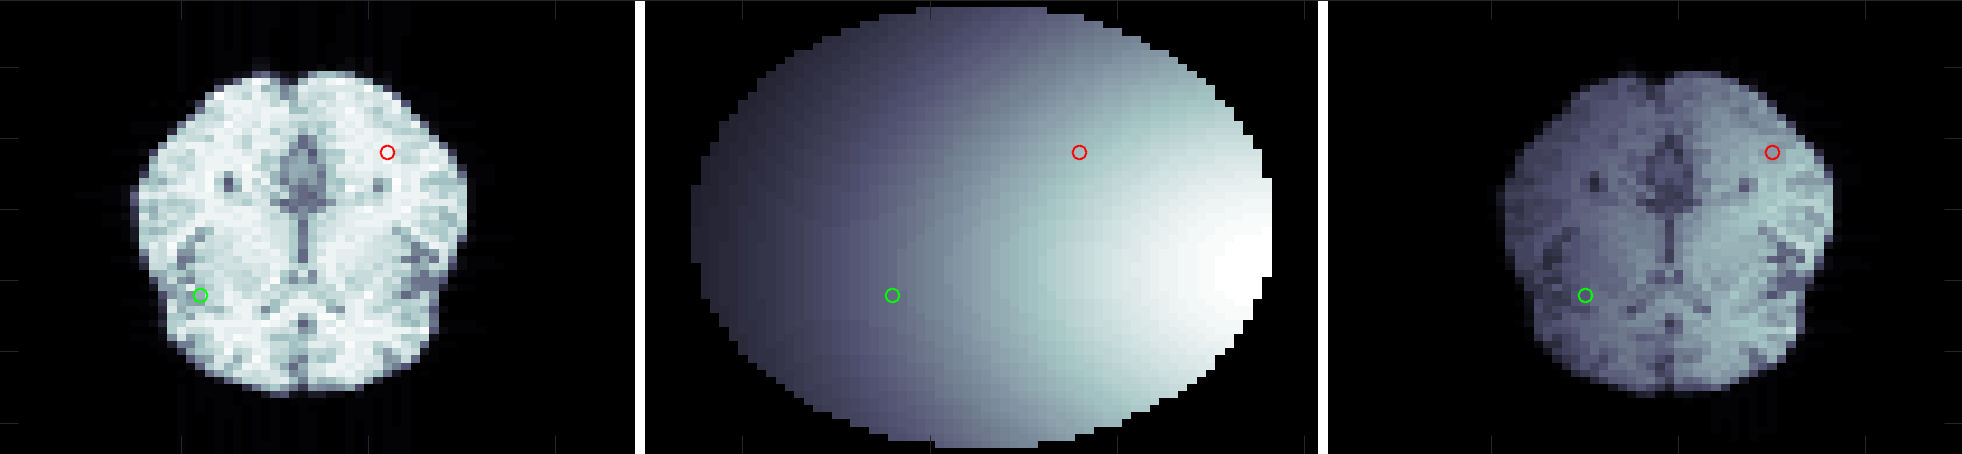
\includegraphics[width=1\textwidth,keepaspectratio]{1coil}
    \caption{From left to right this figure shows: the object, the coil's sensitivity profile and the resulting image as seen by the coil}
    \label{fig:1coil}
\end{figure}

That being said, it is worth investigating how different sensitivity profiles will affect the final reconstruction. Consequently, for this project we have created sensitivity maps that resemble the ones used in parallel imaging techniques. We have opted for a circular geometric placement around the object of interest, with each individual channel being equally apart from its nearest neighbours. Also, we have chosen to spatially vary their sensitivities by modelling a 2D normal distribution which is centered on the channel's position and can have various standard deviations. An example of 2, 4, 6, 8 and 16 channel arrays with sensitivity maps of similar standard deviations is given in Figure~\ref{fig:brainsAndCoilsDistrib}. Moreover, the maps are not spatially varying on the third axis, as the focus for this project was on reconstructing individual slices.

\begin{figure}[H]
    \centering
    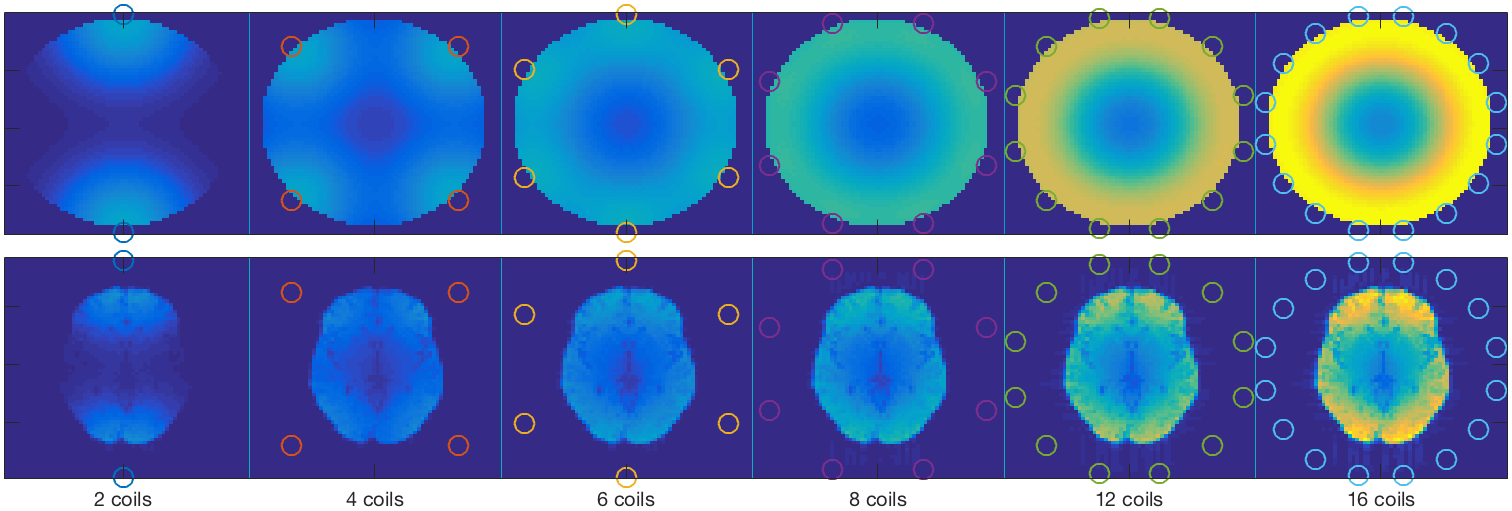
\includegraphics[width=1\textwidth,keepaspectratio]{brainsAndCoilsDistribn2}
    \caption{The 2, 4, 6, 8, 12 and 16 channel arrays used throughout this thesis}
    \label{fig:brainsAndCoilsDistrib}
\end{figure}

As stated before, parallel imaging reconstructions work better when the sensitivity profiles of the channels are spatially varying on the phase-encoding axis, which, in our case, is the y- (vertical) axis of the object. For this reason, as can be seen in Figure~\ref{fig:brainsAndCoilsDistrib}, for the arrays which are made up of 2, 4, 6 and even 8 coils, their geometrical position was chosen such that their spatial variation happens primarily along that axis. For arrays where the number of channels is above 8, that requirement is no longer available as some of the channels will be spatially varying on the x- (horizontal) axis primarily. 

\begin{figure}[H]
    \centering
    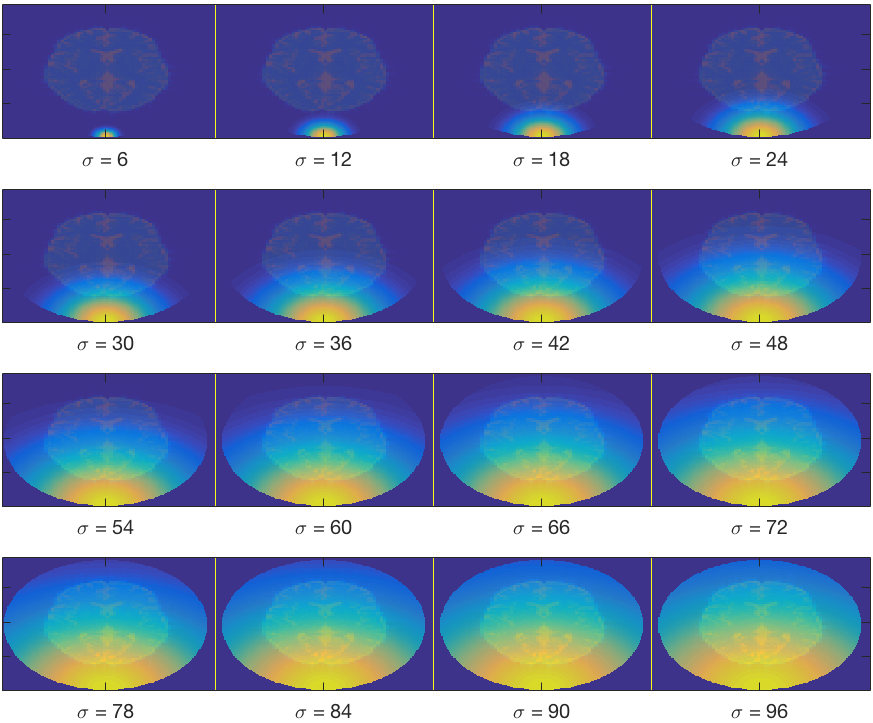
\includegraphics[width=1\textwidth,keepaspectratio]{1coildifsigmas}
    \caption{The sensitivity profiles of an individual channel for increasing standard deviations of the normal distribution used to model their spatial variation}
    \label{fig:1coildifsigmas}
\end{figure}

Another important condition for allowing reasonable reconstructions is to have little overlap between the different coils in order for each individual channel to provide the spatial information needed for a particular area. For this reason, we have chosen to generate sensitivity maps with different coverage sizes to test this theory at the reconstruction step. Figure~\ref{fig:1coildifsigmas} shows the sensitivity profiles of one channel from the 2-coil phased array for different standard deviations of the normal distributions.
%of the individual channels' signal intensity. 
As stated before, the Gaussian distributions model how the signal intensity varies across the object for each individual channel. As expected, a smaller standard deviation will translate into less field-of-view coverage and little overlap, while a higher standard deviation will cover the entire field-of-view and have more overlapping areas between coils. This phenomenon can be visualised in Figure~\ref{fig:2coilsdifsigmas} where the 2-coil array arrangement is presented.

\begin{figure}[H]
    \centering
    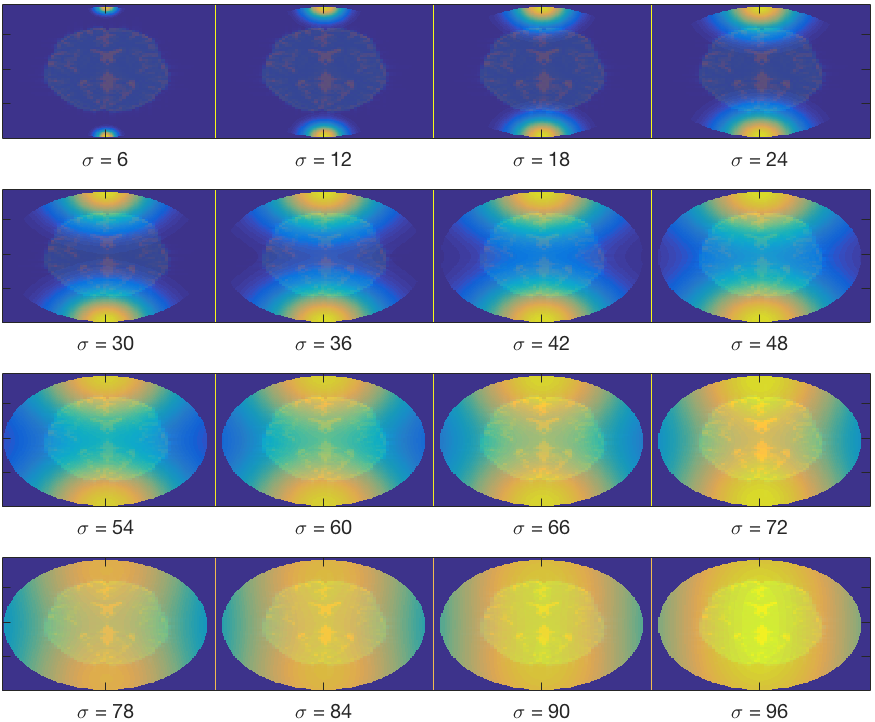
\includegraphics[width=1\textwidth,keepaspectratio]{2coilsdifsigmas}
    \caption{The sensitivity profiles of the 2 channel array}
    \label{fig:2coilsdifsigmas}
\end{figure}

%%%%%%%%%%%%%%%%%%%%%%%%%%
\section{Simulating parallel imaging in POSSUM}
Following on from the previous section which considered the method used to generate coil sensitivity profiles, this section is concerned with how these have been used in the MR simulation pipeline. As mentioned before, the implementation was done within POSSUM, the FMRIB \footnote{Oxford Centre for Functional MRI of the Brain} software tool for simulating realistic MRI and fMRI images. This section will cover in greater detail the MR simulation process when coil sensitivity profiles are present.

To begin with, we will discuss how the signal model is implemented in POSSUM. The simulation process is based on solving the Bloch equations for each individual object voxel at each time point. The overall signal is then calculated as a sum over all magnetization vectors given by the following formula:

\begin{equation} \label{eq:41}
    S(t) = \int_{sample} M_{\perp} (\vec{r}, t) d \vec{r}
\end{equation}
which can be approximated with high accuracy with its discrete form:

\begin{equation} \label{eq:42}
    S(t) = \sum_{j \in \Lambda} \sum_{\vec{r}_0 \in \Omega} s_j (\vec{r}_0, t)
\end{equation}
where $\Omega$ is the set of all object voxels and $\Lambda$ is the set of all tissue templates. 

Therefore, the final signal at time $t$ is given by the sum over all signals $s_j (\vec{r}_0, t)$ coming from the $j$th tissue component at position $\vec{r}_0$ in the input object at time $t$. This is a nice property of the simulator as it allows for tracking of the signal through time and it also allows for various realistic scanning conditions to be implemented. Out of many such scenarios, a few examples can be mentioned: $B_0$ inhomogeneities, RF inhomogeneities and also receiver coil sensitivity profiles can be investigated.

That being said, the first step towards simulating parallel imaging in POSSUM was to add an extra component to the signal calculation. In equation \ref{eq:41} a simplification has been made by considering the receiver coil's sensitivity against the magnetization vector generated by each point of the sample to be equal, and was therefore discarded. In reality, the head coils have an intrinsic sensitivity map which we want to simulate and use. Thus, equation \ref{eq:41} becomes:

\begin{equation} \label{eq:43}
    S(t) = \int_{sample} M_{\perp} (\vec{r}, t) B(\vec{r}) d \vec{r}
\end{equation}
which, again, can be approximated with its discrete version:

\begin{equation} \label{eq:44}
    S(t) = \sum_{j \in \Lambda} \sum_{\vec{r}_0 \in \Omega} s_j (\vec{r}_0, t) B(\vec{r}_0)
\end{equation}

As discussed before, the final signal is the sum over all signals coming from every point in the input object. This object, representing a brain, is made up of 192 x 192 x 192 cuboid elements (of 1mm x 1mm x 1mm in size) which contain information about the properties of each tissue type ($T_1$ and $T_2^*$ relaxation times and spin density $\rho$). These values are uniform across each object voxel. 

That being said, the sensitivity maps of each receiver coil were generated to be of the same size as the input object. In our case, each sensitivity profile is a three dimensional object of 192 x 192 x 192 in size and it contains, for each object voxel, a value between 0 and 1. This value represents how sensitive that respective coil is to the signal coming from a certain spatial location within the object.

As far as different phased-array arrangements is concerned, we have chosen to generate each sensitivity map separately. This implies that, for each mixture of channel positions, we are generating the required number of sensitivity maps and we are running POSSUM with each of them separately. This design choice allows for faster simulations as the software can be run on a cluster system and each coil will be treated by a different job, in parallel.

In practical terms this translates into running the newly enhanced \texttt{possumX} (the CLI\footnote{command line interface} for POSSUM) with the \texttt{-p} flag followed by the number of coils desired. When doing so, you should make sure the simulation folder contains the sensitivity profiles generated earlier. By default, when the flag is not present, POSSUM calculates the signal by considering an overall homogeneous sensitivity profile. At the end of a simulation, the simulation directory will contain as many output images as there were coils. That being said, an \textit{n}-coil arrangement will produce a collection of \textit{n} images for a given standard deviation. An example of such a simulation for a 6-coil array and with a standard deviation of the Gaussian distribution which models the sensitivity profile of $\sigma = 72$ can be seen in Figure~\ref{fig:brains1sigma}.

\begin{figure}[H]
    \centering
    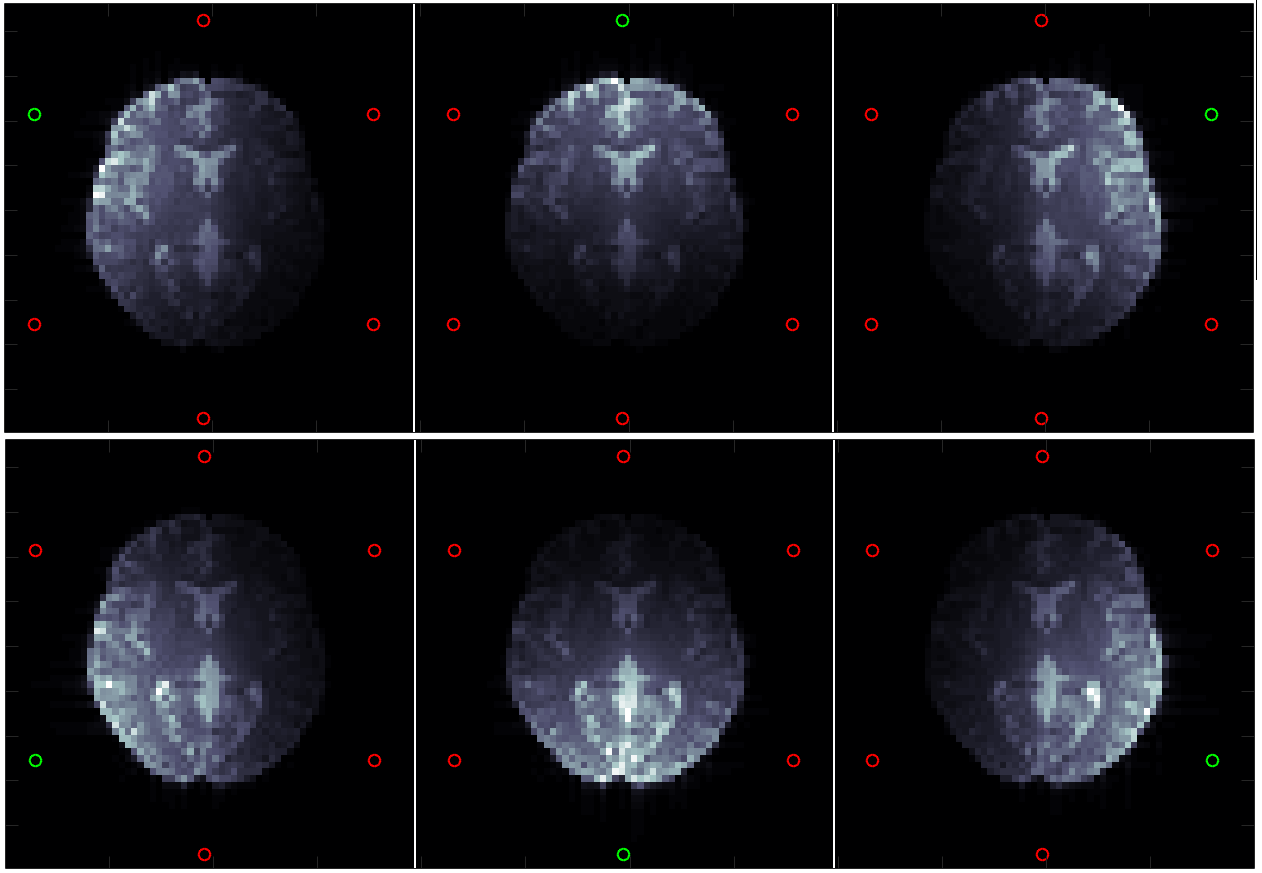
\includegraphics[width=1\textwidth,keepaspectratio]{brains1sigma}
    \caption{A 6-channel phased-array coil simulation for sensitivity maps of $\sigma = 72$}
    \label{fig:brains1sigma}
\end{figure}

%An example of a 4-array coil simulation (positioned North-South-West-East) which was run with the EPI sequence can be seen in Figure~\ref{fig:4arraycoil}.
% 
% \begin{figure}[H]
%     \centering
%     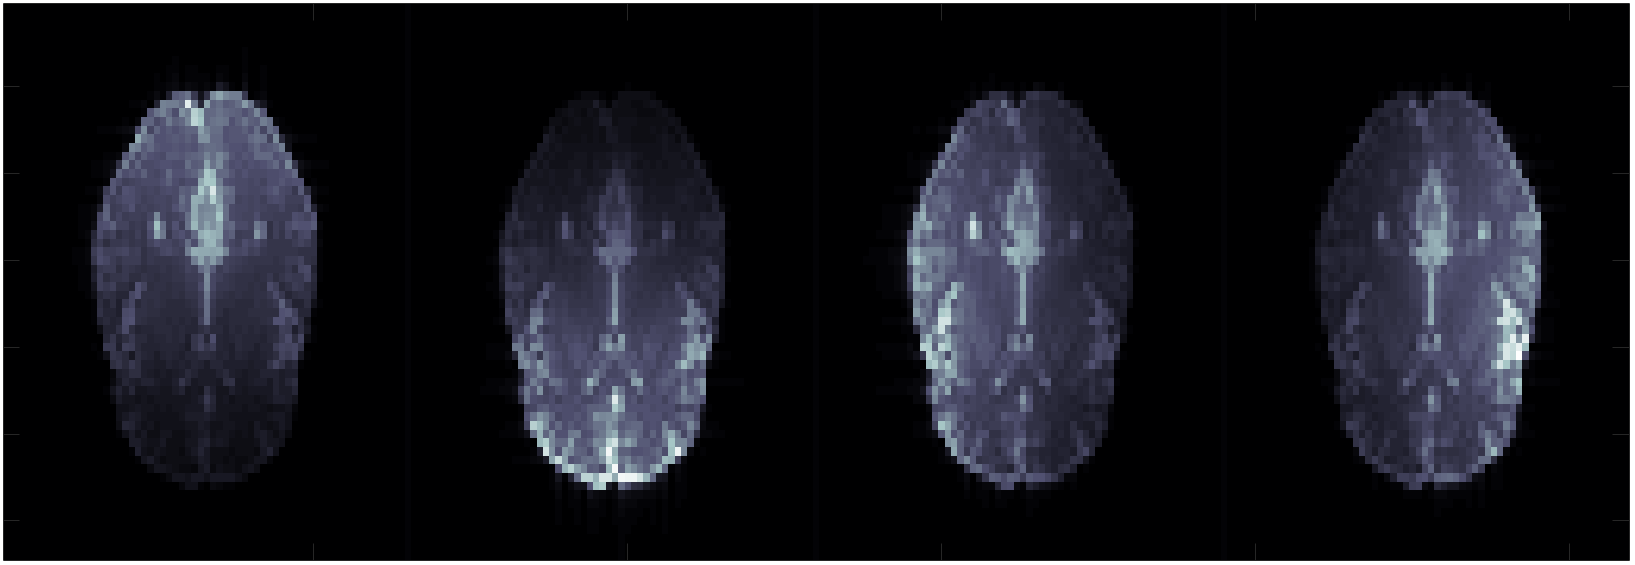
\includegraphics[width=1\textwidth,keepaspectratio]{4arraycoil}
%     \caption{todo caption }
%     \label{fig:4arraycoil}
% \end{figure}

%%%%%%%%%%%%%%%%%%%%%%%%%%
\section{Simulating aliased images in POSSUM}
\label{ch4sectionaliased}
Parallel imaging techniques have been developed in order to accelerate scanning time. As stated before, in order for this to happen, phase-encoding steps can be skipped. The missing information can be recovered by means of coil sensitivity profiles. We have seen in the previous sections how these were generated and then used to reconstruct the final MR image. In this section the focus will be on simulating an undersampled k-space by means of skipping phase-encoding steps.

When an MRI acquisition is performed, each of the scanner's hardware parts, such as the gradients and RF coils, are being controlled by a set of commands sent from the main console. The recipe for how and when to activate different magnetic fields within the scanner is called a pulse sequence. The simulation software has a similar approach as the real scanner in terms of controlling the RF fields, the gradient fields and the receiver electronics. 

To put it more simply, POSSUM defines the pulse sequence as a set of values at discrete time points for the gradient fields and the RF fields. On top of these, the matrix also contains values of $0$s or $1$s for signal read-out ($1$ for when signal should be read and $0$ otherwise). The pulse sequence used by POSSUM is therefore in matrix form which means that user-defined sequences are allowed as long as they preserve the same writing standard. An example was shown in Figure~\ref{fig:pulseseqtable}.

One of the pulse sequences defined by POSSUM is EPI (Echo Planar Imaging) as this software tool was initially designed for fMRI simulations. EPI is a fast imaging technique that allows entire slices to be acquired in one single shot. This means that the entire k-space matrix can be acquired after one RF pulse (for GE-EPI). A diagram of a standard GE-EPI pulse sequence in shown in Figure~\ref{fig:episequence} together with the corresponding k-space acquisition. 

\begin{figure}[H]
    \centering
    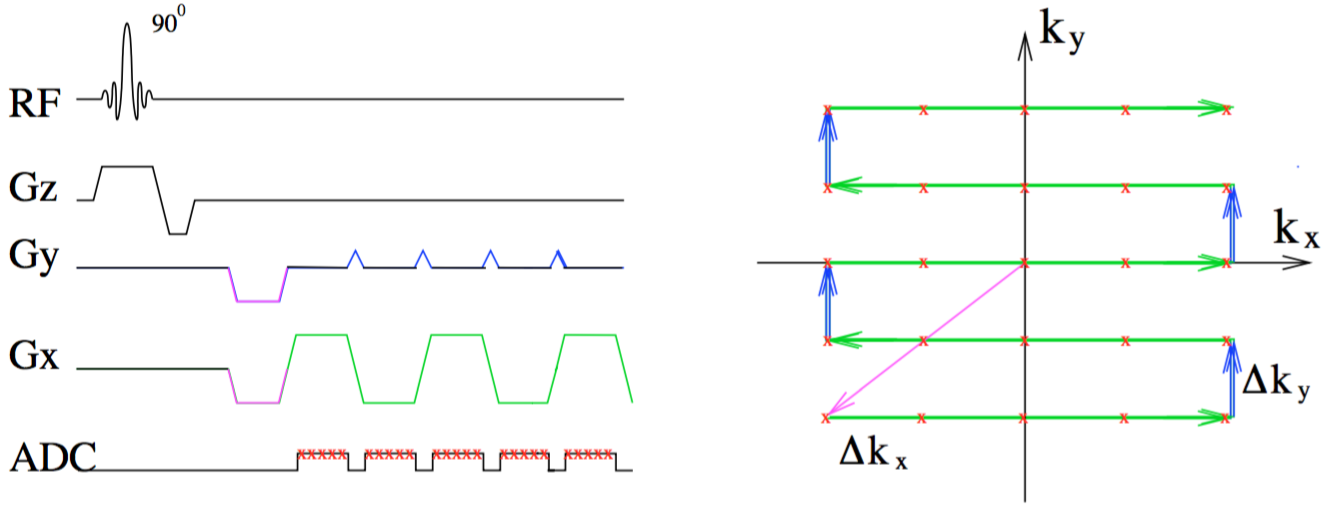
\includegraphics[width=1\textwidth,keepaspectratio]{episequence}
    \caption{Standard echo planar imaging (EPI) sequence together with the corresponding k-space sampling. Figure courtesy of \cite{Drobnjak07}}
    \label{fig:episequence}
\end{figure}

In order to accelerate the image acquisition process, two steps need to be done. First, the phase encoding gradients need to be increased by the same amount as the parallel imaging acceleration factor R. For example, to halve the acquisition time ($R = 2$), the phase encoding gradients, or "blips", need to become twice as strong as in a normal acquisition. This will translate into $\Delta k_y' = 2 \Delta k_y$ which is the same as skipping every other k-space line. Second, the number of k-space lines acquired needs to be decreased by the same factor R. This means that for a standard 128 x 128 k-space matrix, when using $R = 2$, the final k-space size will be reduced to 64 x 128, halving the amount of phase-encoding lines.

As we have discussed before in Chapter~\ref{chapterlabel2}, the 
k-space sampling interval in the phase-encoding direction is inversely proportional to the field-of-view: $\Delta k_y = \frac{1}{FOV_y}$ (eq. \ref{eq:270}). Also, the image spatial resolution is inversely proportional to the highest spatial frequency sampled in k-space. In mathematical terms, this translates into $\Delta y = \frac{1}{N_y \Delta k_y} = \frac{1}{2 k_{y,max}}$ (eq. \ref{eq:273}). This means that for an acceleration factor $R = 2$, the sampling interval will increase twofold leading to: $\Delta k_y' = 2 \Delta k_y = \frac{2}{FOV_y} = \frac{1}{\frac{FOV_y}{2}} = \frac{1}{FOV_y'}$. Therefore, the new field of view is half of the original one: $FOV_y' = \frac{FOV_y}{2}$. This leads to aliasing in the final images as the \textit{Nyquist-Shannon} condition is not met anymore.

This phenomenon was simulated in POSSUM. The results were as expected and the final reconstructions showed aliased images. An example of a simulation ran with an acceleration factor $R = 2$, meaning a halved field-of-view, can be found in Figure \ref{fig:figaliased}. The 6-channel array used was presented in Figure~\ref{fig:brains1sigma}.

\begin{figure}[H]
    \centering
    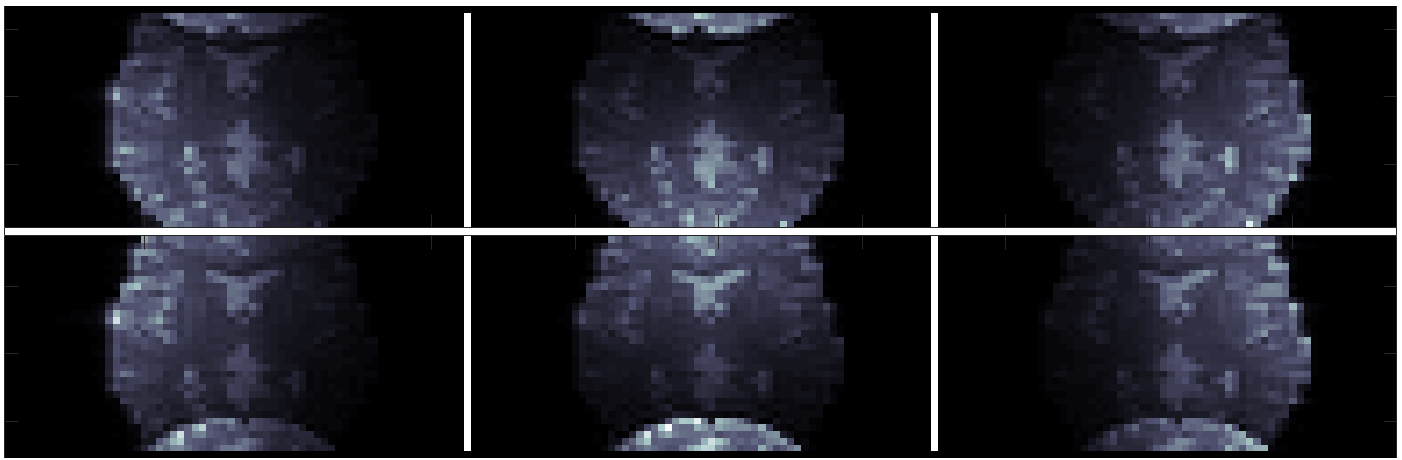
\includegraphics[width=1\textwidth,keepaspectratio]{figaliased}
    \caption{POSSUM simulating aliased images with a 6-coil array and with an acceleration factor $R = 2$}
    \label{fig:figaliased}
\end{figure}

For all our simulations that will be presented in the next chapter, we have used the (parallel imaging capable) Echo Planar Imaging pulse sequence. This is one of the most common MRI pulse sequences for single-shot k-space acquisitions, as it can acquire up to 128 phase-encoding steps in 20-100ms. Although it provides excellent temporal resolution and it is the most popular sequence for fMRI studies, the image quality can be poor \cite{Farzaneh1990}. This is due to various problems associated with this sequence such as signal dropout at the interfaces between different tissue types where magnetic susceptibility differences appear. It was therefore proposed by Griswold et al \cite{Griswold1999} and by Bammer et al \cite{Bammer2001} that the use of parallel imaging techniques can reduce image artifacts to a level that was only accomplished by interleaved EPI acquisitions \cite{Schmiedeskamp2010}. Although the investigation of whether this holds true with simulation is not the scope of this project, it could become future work.

%%%%%%%%%%%%%%%%%%%%%%%%%%
\section{SENSE reconstruction}
\label{ch4sectionsense}
So far we have seen how coil sensitivity maps were generated for various phased-array channel arrangements and how they can be used in POSSUM to simulate signal acquisition with coils that have a non-homogeneous spatial sensitivity. We have also discussed the simulation of aliased images in our MRI software tool. These two together are part of the parallel imaging pipeline being developed in POSSUM. This next section is concerned with the reconstruction algorithm that uses the folded images and the coil sensitivity profiles in order to retrieve the original image.

Pruessmann et al showed in 1999 that for 2D Fourier imaging with k-space coefficients being sampled in a Cartesian fashion, scan time can be reduced by increasing the relative distance between adjacent sampling positions \cite{Pruessmann1999}. This will invariably lead to a reduction of the FOV, causing folding in the final images. However, this is where parallel imaging reconstruction algorithms come into place. As we have discussed before, there are a couple of ways to recover full FOV images from aliased ones. One of these algorithms which does reconstruction in the image domain is SENSE and it is the topic of our discussion in this section.

The main idea behind SENSE (sensitivity encoding) is to use the sensitivity maps of the individual receiver channels in order to 'unfold' the aliased images. It therefore relies on two separate inputs: the set of images reconstructed for each of the individual coils from the multi-coil array and the collection of sensitivity profiles of these channels. Having these two, reconstruction works as long as there are more channels than folded intensities \cite{Pruessmann1999}. 

To better understand this phenomenon, let us follow an example. In Figure~\ref{fig:senserecbrains} we see on the left-hand side of the image the object of interest: a brain. Next, the middle column shows how each individual channel sees the object: every intensity value for each location in the image is weighted by the coil's sensitivity at those coordinates. Finally, in the right hand side column, we can see the reconstructed (aliased) images for each channel. In our example, acquisition was performed with an acceleration factor $R = 2$, which means that the final field-of-view will be halved. For qualitative purposes, the images shown are full FOV, for the purpose of seeing exactly where parts of our initial object are juxtaposing.

Figure~\ref{fig:senserecbrains} also shows that the two locations $A$ and $B$ are 'folded' in the final images, both intensities contributing to the final value found in the aliased images. Therefore, as long as the two locations experience different sensitivity weightings by each of the channels in the phased-array coil, a good reconstruction can be performed.

\begin{figure}[H]
    \centering
    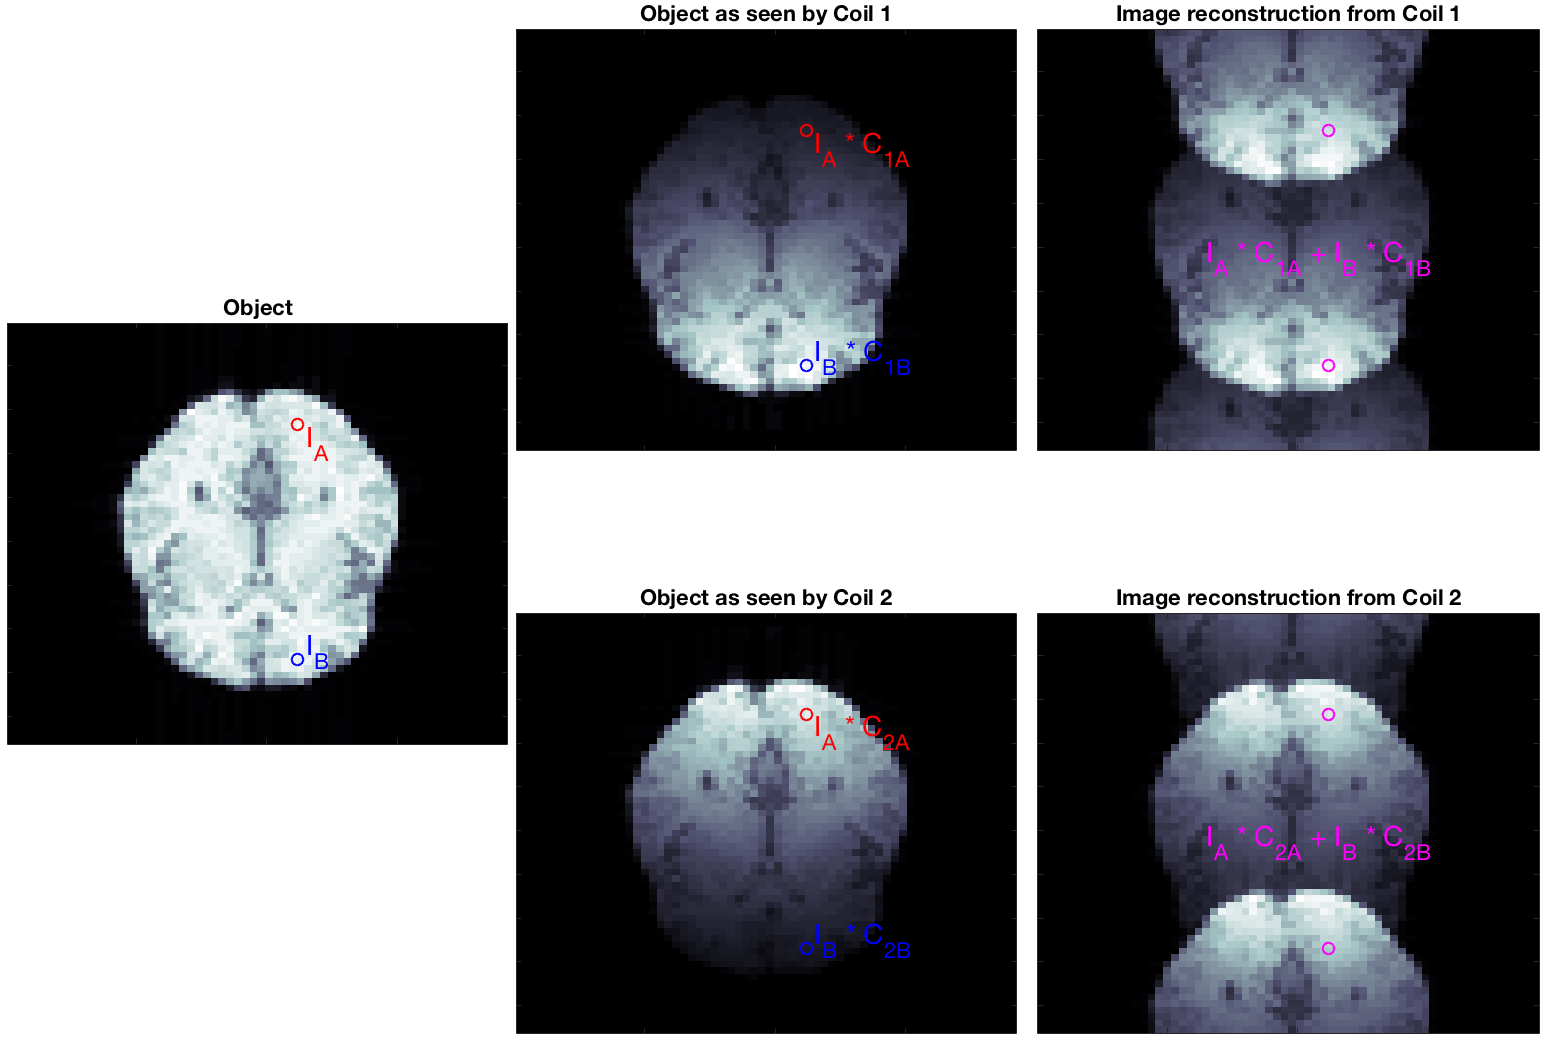
\includegraphics[width=1\textwidth,keepaspectratio]{senserecbrains}
    \caption{Aliased images from two coils. The signal value at folded locations shown in magenta is the sum between the object values at the two locations, A and B, for each coil.}
    \label{fig:senserecbrains}
\end{figure}

Now, in order to express this concept mathematically, a few other aspects need to be discussed. First, we take into account the fact that the acceleration factor $R$ contributes to a reduction of the FOV from $L$ to $L/R$, where $L$ is the length of our full field-of-view. Second, the total number of replicates (overlapping signals) at each voxel location is $N_A = 2 N(AR/L) + 1$, where $N(u) = -[(1-u)/2]$ is defined to be the \textit{largest integer less than or equal to} operation and $A$ is the length of the FOV which encompasses the object of interest. Third, we define the number of channels in the coil array as $N_c$ and the sensitivity profiles for each of them as $C_j$, for $j \in [0, N_c-1]$. Finally, for each location $y$ in the image, we can write the signal intensity $I(y)$ at that location as a sum of the weighted intensity values coming from each of the aliased locations. 

\begin{equation} \label{eq:45}
    I_j(y)  = \sum_{n=0}^{N_A-1} C_j(y+nL/R) M(y+nL/R)
\end{equation}
where $M$ holds the real intensity values from the object of interest for each location $y$.

Now, if $N_c \geq N_A$, the system of equations can be solved and $M(y+nL/R)$ can be retrieved. Writing $I$ as an $N_c$ x $1$ matrix, $C$ as an $N_c$ x $N_A$ matrix and $M$ as an $N_A$ x $1$ matrix, we get:

\begin{equation}
    I = \left[
    \begin{array}{ c }
          I_0(y) \\
          I_1(y) \\
          \cdots \\
           I_{N_c-1}(y)
    \end{array}
    \right],
\end{equation}

\begin{equation}
    C = \left[
    \begin{array}{ c c c }
          C_0(y) & \cdots & C_0(y+(N_A-1)L/R)  \\
          \cdots & \cdots & \cdots \\
          C_{N_c-1}(y) & \cdots & C_{N_c-1}(y+(N_A-1)L/R)
    \end{array}
    \right]
\end{equation}
and
\begin{equation}
    M = \left[
    \begin{array}{ c }
          M(y) \\
          M(y+L/R) \\
          \cdots \\
          M(y+(N_A-1)L/R)
    \end{array}
    \right]
\end{equation}

We can therefore write equation \ref{eq:45} in matrix form as:

\begin{equation}
    I = C M
\end{equation} 

In order to recover the unfolded image, a Moore-Penrose pseudo-inverse is performed:

\begin{equation}
    M = (C^T C) ^{-1} C^T I =  C^\dagger I
\end{equation}

The reconstruction step of the pipeline was implemented in MATLAB following a medical imaging reconstruction tutorial\footnote{\url{https://web.stanford.edu/class/ee369c/restricted/Solutions/assignment_4_solns.pdf}} offered by Stanford. The algorithm requires 3 inputs: the collection of aliased images, the set of coil sensitivity profiles and the acceleration factor R.

Moreover, a function for calculating the coil "g-factor" is implemented as well. The mathematical concepts behind the coil geometry factor have been presented in Section \ref{sect:senserec}. Nevertheless, it is an important notion that needs to be reminded. The coil "g-factor" is a measure of the added noise brought about the combination of multiple coils. It can be calculated with the following equation:

\begin{equation}
    g_y = \sqrt{ [(C^T \Psi^{-1} C )^{-1}]_{yy} (C^T \Psi^{-1} C )_{yy} }
\end{equation}

where $g_y$ is the g-factor at location $y$, $\Psi$ is the noise correlation matrix and $C$ is the sensitivity encoding matrix. This factor also influences the signal-to-noise ratio in the final reconstructed images. The signal drop is given by the next equation:

\begin{equation}
    SNR_{SENSE} = \frac{SNR_{Original}}{g \sqrt{R}}
\end{equation}

where $R$ is the acceleration factor and $SNR_{Original}$ is the signal-to-noise ratio of a similar MRI image taken without parallel imaging.

The simulations which will be presented in the next chapter will use the Stanford tutorial to perform SENSE reconstructions and g-factor maps for a combination of array channels, sensitivity profiles and acceleration factors.














\chapter{Results}
\label{chapterlabel5}

The aim of this section is to both test the proposed parallel imaging pipeline and the SENSE reconstruction algorithm for different scenarios. First, the proposed pMRI technique is performed using an acceleration factor $R = 1$ (no phase-encoding lines are skipped) for all defined sensitivity maps and for all previously described coil configurations. Second, the quality of reconstruction is tested for increasing acceleration factors. Finally, the outcome of the reconstruction when increasing levels of noise are added to the sensitivity profiles is presented. 
%Finally, motion during acquisition time is considered and the proposed pipeline is again investigated. 

%%%%%%%%%%%%%%
\section{Enhancing POSSUM with multi-coil acquisition}
This section is concerned with the proposed multi-coil acquisition pipeline. First, the design of the experiment is presented, followed by results and further discussion.

\subsection{Design}
The first step towards enhancing POSSUM with parallel imaging capabilities is to enable it to receive as input the sensitivity maps of the coils. For this reason, the current section is concerned with generating the coil sensitivity profiles for all subsequent simulations. Moreover, SENSE reconstructions will be performed without skipping phase-encoding lines (full FOV images).

As stated before, the object used as input in POSSUM, representing a brain, consists of 192 x 192 x 192 cuboid elements, with physical dimensions of 1mm x 1mm x 1mm, containing information about the properties (spin density $\rho$, $T_1$ and $T_2^*$ relaxation times) of each tissue type (WM, GM and CSF). For this reason, the sensitivity maps of each receiver channel were generated to be of the same size as the input object and to contain, for each voxel within, a value between 0 and 1 representing the sensitivity of the signal originating from that particular spatial location (a value of 1 represents maximum sensitivity, whereas for 0 no signal is perceived).

In compliance with realistic sensitivity profiles, the design of choice was to enforce the spatial variations of the sensitivity values to take a 2 dimensional Gaussian form of isotropic cross-section. Various standard deviations of the normal distribution were used to generate the sensitivity profiles, while different channel combinations were generated by shifting the center of the Gaussian to a different spatial location within a slice. 

Under these circumstances, the parallel imaging pipeline was tested with 2, 4, 6, 8, 12 and 16 phased-array coil combinations for various standard deviations of the normal distributions ranging from 6 to 96. The results are shown in the following section.

\subsection{Results}
Figure~\ref{fig:1coildifsigmas2} shows the coil sensitivity profiles as generated for this project. For qualitative reasons, the sensitivity profiles have been overlaid on top of the object of interest (the brain used as input for our simulations). As stated before, we have chosen to spatially vary their sensitivities by modelling normal distributions of various standard deviations. The $\sigma$ values go from $6$ to $96$. As can be seen, higher standard deviations will translate into more field-of-view coverage, while a lower standard deviation will only affect part of the domain. 

In order to test the reconstruction accuracy, we have chosen to create various arrangements of these sensitivity profiles. In all of our subsequent simulations, the number of channels chosen were: 2, 4, 6, 8, 12 and 16. Figure~\ref{fig:2coilsdifsigmas2} shows the 2-channel arrangement while the others are presented in Appendix~\ref{appendixlabel1}.

\begin{figure}[H]
    \centering
    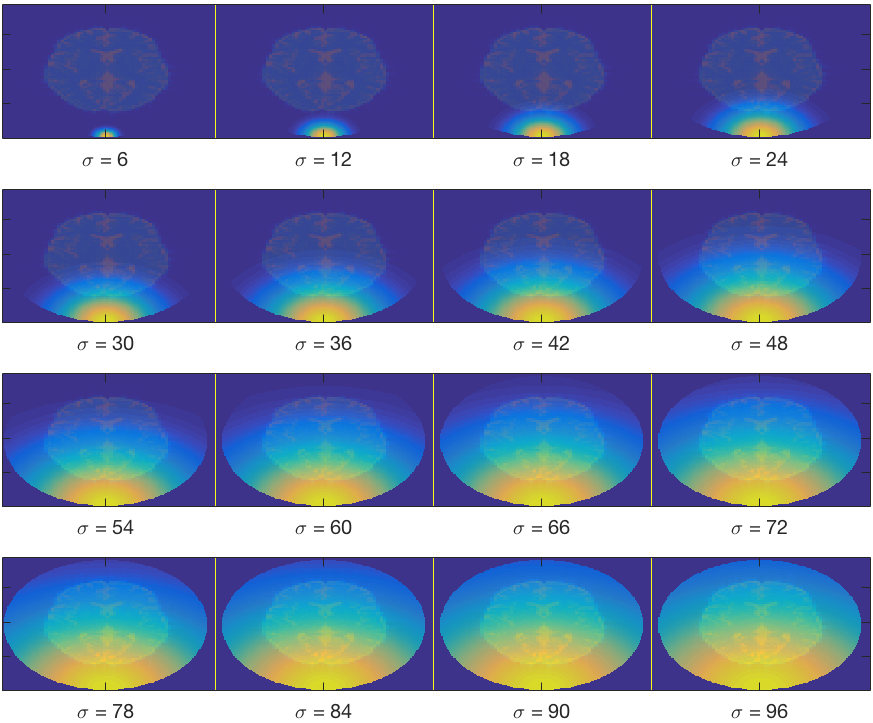
\includegraphics[width=.85\textwidth,keepaspectratio]{1coildifsigmas}
    \caption{Coil sensitivity profiles used in simulations}
    \label{fig:1coildifsigmas2}
\end{figure}

\begin{figure}[H]
    \centering
    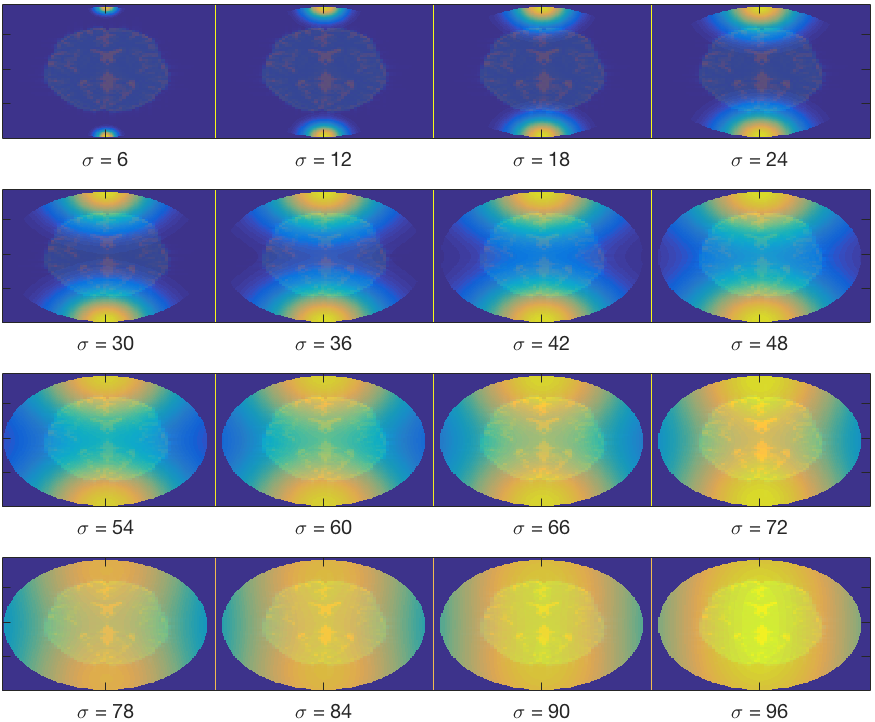
\includegraphics[width=.85\textwidth,keepaspectratio]{2coilsdifsigmas}
    \caption{Coil sensitivity maps of the 2-channel phased-array coil}
    \label{fig:2coilsdifsigmas2}
\end{figure}

All of the presented maps have been used as inputs to POSSUM in order to generate \textit{sensitivity-weighted} reconstructions. Due to the increasing computational time as the number of channels gets higher, the design of choice was to run POSSUM for each sensitivity map independently. This allows for faster simulations as on a cluster system each coil will be treated by a different job, in parallel. Moreover, the complexity of the array (coil location and number of channels) will not influence the running time significantly.

\begin{figure}[H]
    \centering
    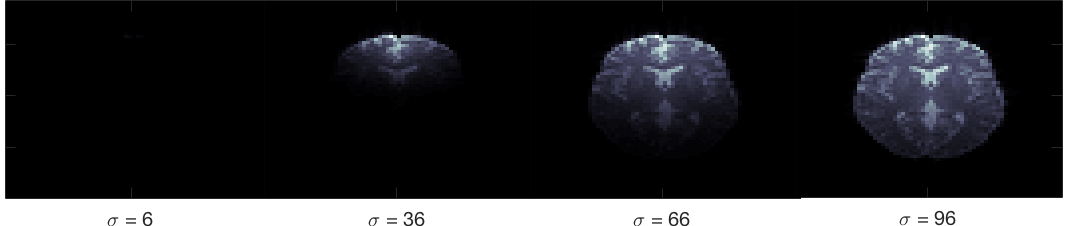
\includegraphics[width=1\textwidth,keepaspectratio]{brainsdifsigmas}
    \caption{Results of POSSUM enhanced simulations for increasing standard deviations of the sensitivity profiles of one channel}
    \label{fig:brainsdifsigmas}
\end{figure}

Figure~\ref{fig:brainsdifsigmas} shows the output of 4 simulations which were run for 4 of the previously described sensitivity maps. The lowest and highest standard deviations used are shown in this figure to better visualise the two extremes. Moreover, the figure only shows one output image per simulation corresponding to a coil positioned in the upper part of the object. Reconstructions of the final images given all coil combinations and different sensitivity maps are presented in Figure~\ref{fig:1brainsR1rec}. To better visualise the quality of reconstruction, Figure~\ref{fig:1brainsR1ssd} shows the sum of squared differences between each reconstruction and the original image. The latter was simulated with the equivalent of a homogeneous sensitivity map and with full FOV acquisition.

\subsection{Discussion}
In this first experiment we showed that multi-coil acquisition is now possible with POSSUM. The first step towards this goal was to create a collection of different sensitivity maps showing different amounts of object coverage in terms of coil sensitivity. SENSE reconstruction was also performed with $R = 1$ as was described in Section~\ref{ch4sectionsense}. 

Figure \ref{fig:1brainsR1rec} shows the SENSE reconstructions performed for increasing standard deviations of the sensitivity profiles and for all coil combinations. The trend shows an increased performance as coil geometry gets better. For example, for a 2-channel array, the algorithm is unable to reconstruct the image for the same sensitivity profile used in the 4/6/8/12/16-channel arrays. Moreover, a convergence seems to be reached in the last column, where all coil combinations perform well. This is backed up by Figure \ref{fig:1brainsR1ssd} which shows a similar trend. 

\begin{figure}[H]
    \centering
    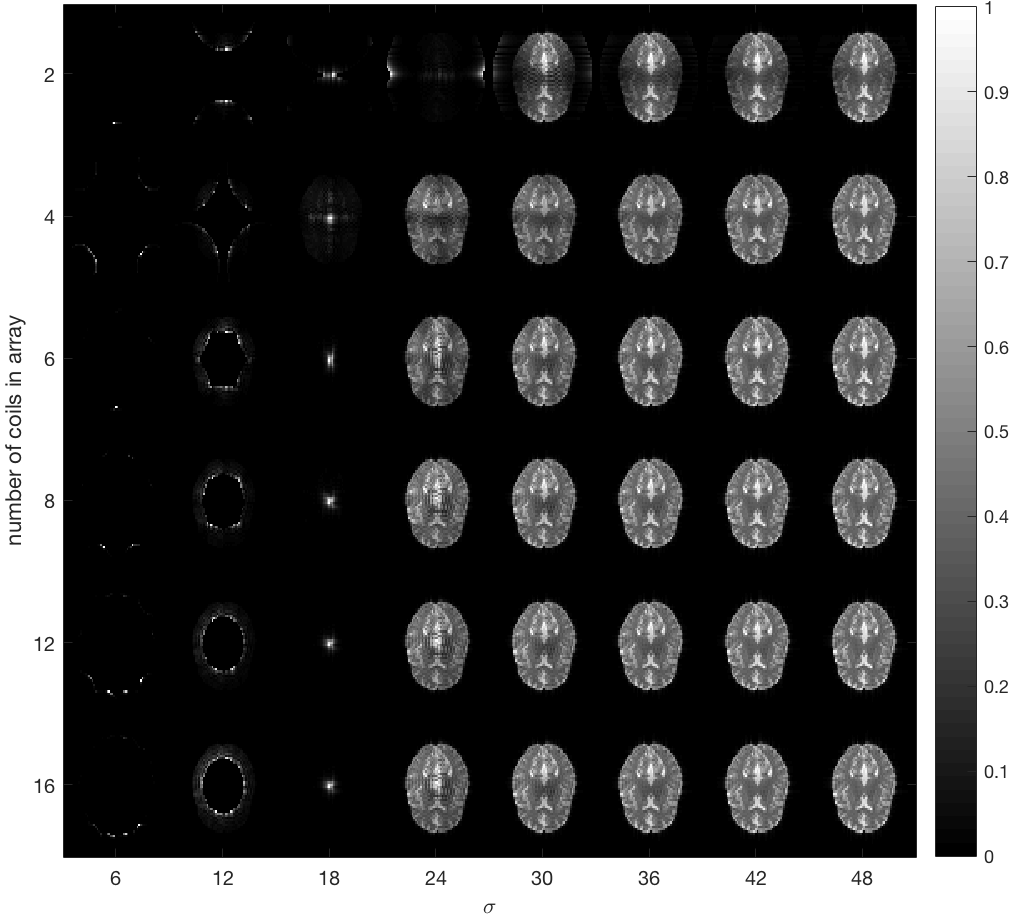
\includegraphics[width=1\textwidth,keepaspectratio]{1brainsR1rec}
    \caption{Reconstruction of multi-coil acquisitions for different numbers of channels and for different standard deviations of the associated sensitivity maps}
    \label{fig:1brainsR1rec}
\end{figure}

In conclusion, this first experiment tells us that multi-coil acquisition requires a good combination of at least two parameters: the standard deviation of the associated sensitivity map and the geometry of the coil array. As can be seen in Figures \ref{fig:1brainsR1rec} and \ref{fig:1brainsR1ssd}, choosing small standard deviations of the sensitivity profiles will translate into poor or even impossible reconstructions. However, in parallel imaging techniques, too much coverage can also be detrimental as in that case distinguishing between two or more spatial locations would become impossible. This happens because a very smooth sensitivity profile used in conjunction with a high number of channels can mean that many spatial locations within the object of interest will be "weighted" by the same sensitivity value. This will lead to incorrect reconstructions. In the following section, different acceleration factors are considered and SENSE reconstruction is again performed.

\begin{figure}[H]
    \centering
    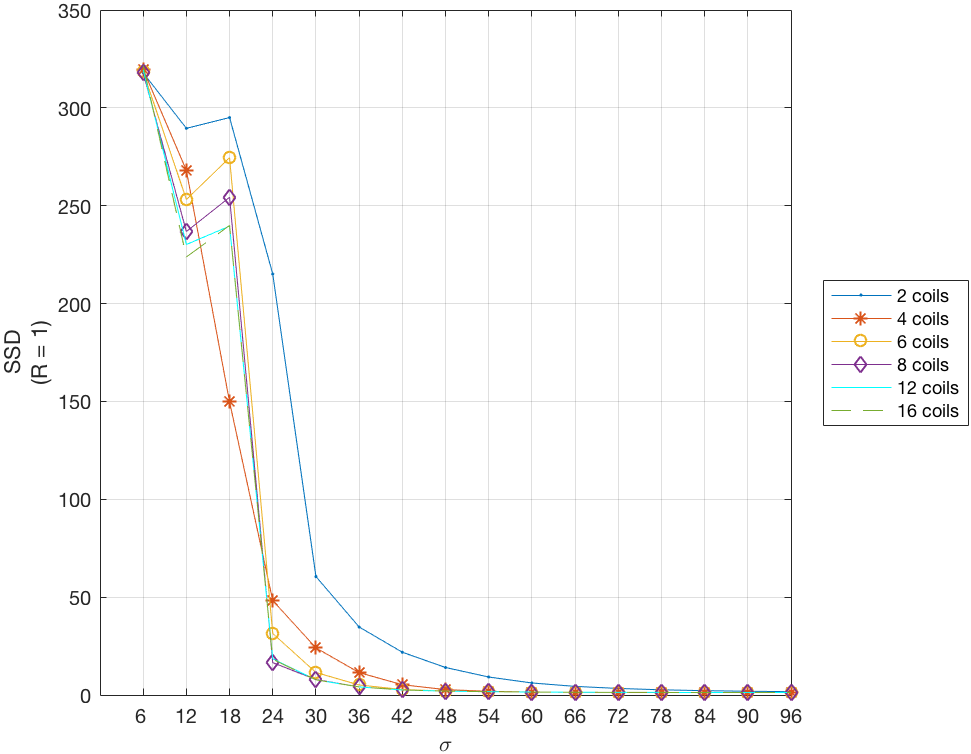
\includegraphics[width=1\textwidth,keepaspectratio]{1brainR1ssd}
    \caption{SSD between original image and the reconstructions coming from each multi-coil acquisitions for different numbers of channels and for different standard deviations of the associated sensitivity maps. The acceleration factor used is $R = 1$. The trend of the plot clearly shows an improvement in reconstruction as the standard deviation of the sensitivity profile and also as the number of channels in the array gets higher.}
    \label{fig:1brainsR1ssd}
\end{figure}

%%%%%%%%%%%%%%%
\section{SENSE reconstructions with different acceleration factors} \label{exp2}
This section is concerned with reconstructions performed with different acceleration factors, more specifically: $R = \left\{1, 2, 3, 4\right\}$. The aim of this experiment is to investigate how the quality of reconstruction is affected by increasing acceleration factors. The experiment design will be discussed first, followed by results and discussion.

\subsection{Design}
The next step towards implementing a parallel imaging pipeline in POSSUM is to enable simulations with undersampled acquisitions in the phase-encoding direction. The method of choice and its implementation in POSSUM was detailed in Section~\ref{ch4sectionaliased}. 

For this experiment 4 acceleration factors, more specifically $R = \left\{1, 2, 3, 4\right\}$, were considered. The sequence under test was an EPI sequence with a $N_x$ x $N_y$ of 64 x 64 sampling steps. In our case, this means that the number of phase-encoding lines acquired was decreased from a full 64 line acquisition, to 32 lines for $R = 2$, to 21 lines for $R = 3$, and, finally, 16 lines when $R = 4$. Higher acceleration factors were not taken into consideration as the amount of information left would have been too low for good reconstructions and are generally not used in clinical practices.

For each of these, simulations were run for all channel array combinations and for all sensitivity profiles presented before, with reconstructions shown in the next subsection. Moreover, as the quality of reconstruction depends on the coil "g-factor", this was also calculated for all possible combinations. As stated before, the "g-factor" is a measure of noise amplification at a given location in the final image and is, therefore, a location-specific indication of how well the signal can be retrieved given a specific coil combination and a certain acceleration factor.

\begin{figure}[H]
    \centering
    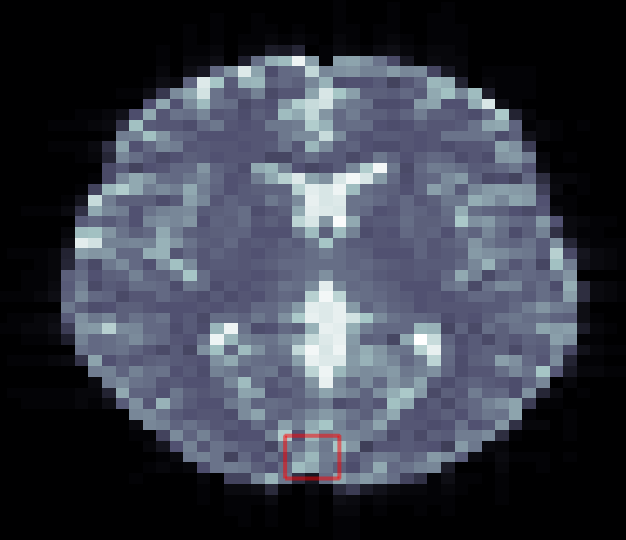
\includegraphics[width=.3\textwidth,keepaspectratio]{roigfact}
    \caption{The chosen ROI for the g-factor calculations}
    \label{fig:roigfact}
\end{figure}

Finally, a region of interest was considered (see Figure~\ref{fig:roigfact}) and the "g-factor", together with the relative decrease in signal-to-noise ratio, was calculated for all coil arrays and all sensitivity profiles.

\subsection{Results}
As stated before, this experiment is focused on the quality of reconstruction for different acceleration factors. Figures \ref{fig:R1brains}, \ref{fig:R2brains}, \ref{fig:R3brains} and \ref{fig:R4brains} show SENSE reconstructions for different acceleration factors, while Figures \ref{fig:R1gfact}, \ref{fig:R2gfact}, \ref{fig:R3gfact} and \ref{fig:R4gfact} show their associated "g-factor" maps.

For visualisation purposes, all "g-factor" maps have been normalised. Still, it is visible from the figures that increasing numbers of coils and also increasing coverage values of the sensitivity profiles will contribute with more uncertainty in the final images as can be seen from the "g-factor" maps and reconstruction figures. 

In addition to qualitatively assessing the reconstructions, a sum-of-squared differences was performed between each SENSE reconstruction and the non-aliased original image for all combinations of values. The results can be seen in Figure~\ref{fig:2SSD} where each plot is a different acceleration factor R.

A quantification of the dependency between our 3 varying parameters (number of coils, acceleration factors and standard deviations) and the quality of reconstruction is shown in Figure~\ref{fig:2gfactor}. It is visible from the plots that an increase in the number of channels used aids the reconstruction. In between plots, it is also visible that higher acceleration factors will decrease the subsequent quality of reconstruction, with a higher plateau reached as $R$ increases. This is due to the fact that when high acceleration factors are used in combination with an increased number of coils, the reconstruction becomes ill-conditioned.

As stated before, the g-factor values also contribute to the overall SNR of the reconstruction. Knowing that $SNR_{SENSE} = \frac{SNR_{Original}}{g \sqrt{R}}$, a region of interest was chosen to calculate the drop in relative SNR due to increasing acceleration factors and, hence, noise contribution coming from different coils. Figure \ref{fig:2SNRsense} shows these results. Again, all three parameters influence the quality of reconstruction. 

%% R1
\begin{figure}[H]
    \centering
    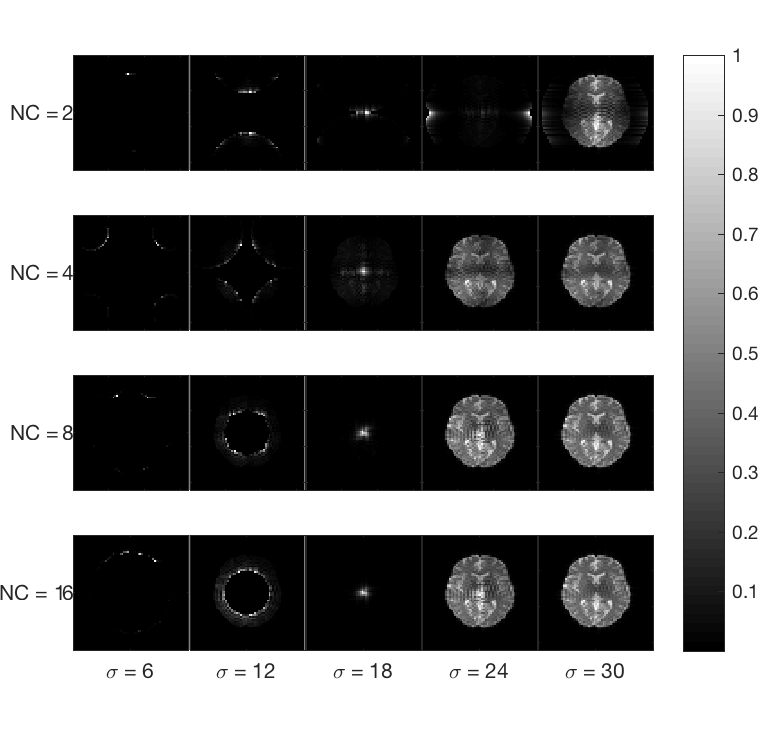
\includegraphics[width=1\textwidth,keepaspectratio]{R1brainsb}
    \caption{SENSE reconstructions for acceleration factor $R = 1$, for increasing numbers of coils on the y-axis and with varying standard deviations of their associated sensitivity profiles on the x-axis}
    \label{fig:R1brains}
\end{figure}

\begin{figure}[H]
    \centering
    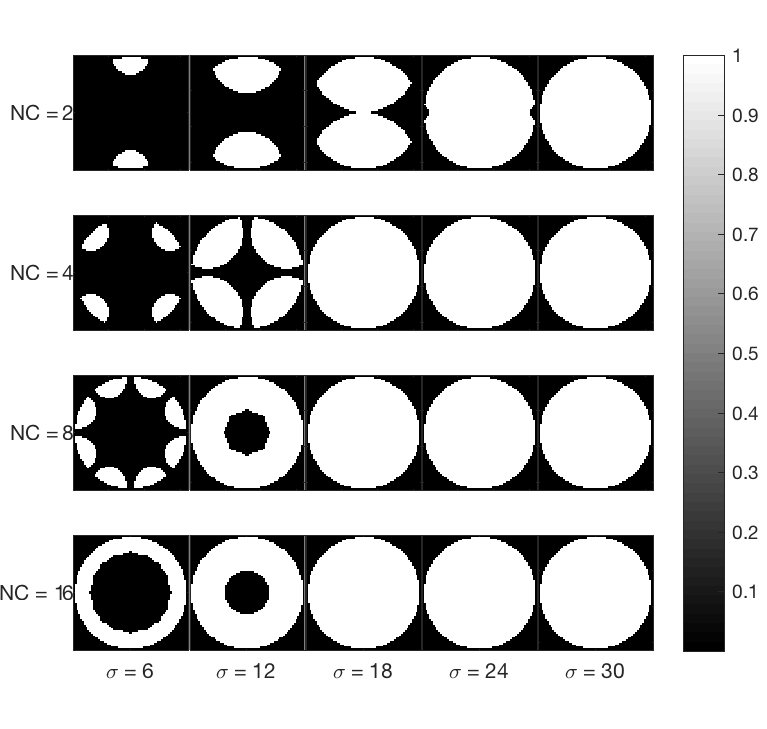
\includegraphics[width=1\textwidth,keepaspectratio]{R1gfactb}
    \caption{g-factor maps for acceleration factor $R = 1$, for increasing numbers of coils on the y-axis and with varying standard deviations of their associated sensitivity profiles on the x-axis}
    \label{fig:R1gfact}
\end{figure}

%% R2
\begin{figure}[H]
    \centering
    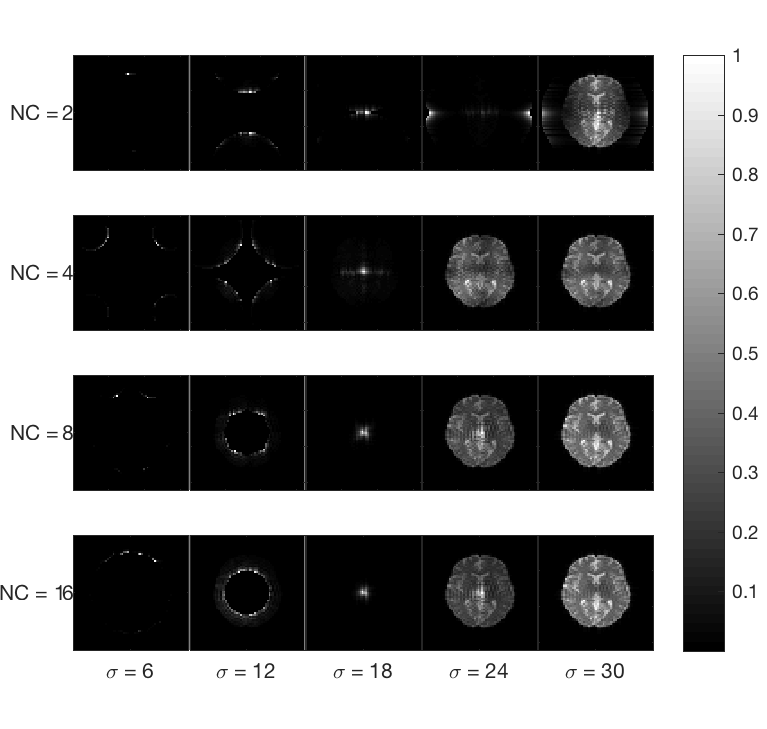
\includegraphics[width=1\textwidth,keepaspectratio]{R2brainsb}
    \caption{SENSE reconstructions for acceleration factor $R = 2$, for increasing numbers of coils on the y-axis and with varying standard deviations of their associated sensitivity profiles on the x-axis}
    \label{fig:R2brains}
\end{figure}

\begin{figure}[H]
    \centering
    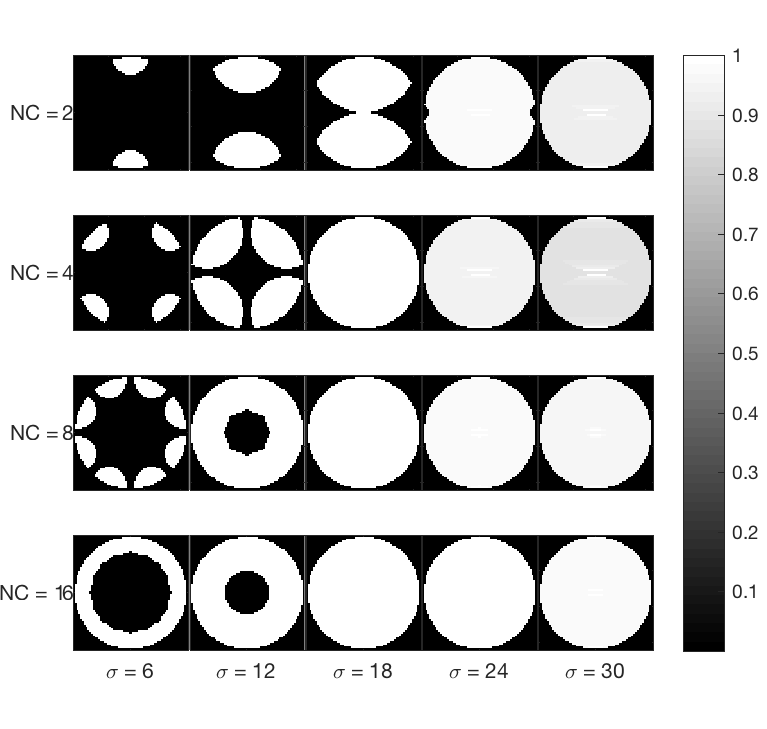
\includegraphics[width=1\textwidth,keepaspectratio]{R2gfactb}
    \caption{g-factor maps for acceleration factor $R = 2$, for increasing numbers of coils on the y-axis and with varying standard deviations of their associated sensitivity profiles on the x-axis}
    \label{fig:R2gfact}
\end{figure}

\subsection{Discussion}
In this experiment we have seen how varying different parameters such as the acceleration factor $R$, the number of coils used in the array and the standard deviations of the associated sensitivity maps can affect the quality of the SENSE reconstruction. 

Now, going back to Figures \ref{fig:R1brains}, \ref{fig:R2brains}, \ref{fig:R3brains} and \ref{fig:R4brains}, which show SENSE reconstructions for increasing acceleration factors, it is interesting to visually inspect the differences between the four results. One striking difference between them is that of the appearance of \textit{residual aliasing} as R is increased. This is, in fact, the main artifact associated with parallel imaging techniques. These artifacts can generally be caused by the bright edges of the images and appear wherever the unfolding process becomes ill-conditioned. 

Moreover, the regions where these artifacts appear are also paired with a decrease in SNR. Indeed, that can be seen in all of our results: Figures \ref{fig:R1gfact}, \ref{fig:R2gfact}, \ref{fig:R3gfact} and \ref{fig:R4gfact} show the locations where the noise caused by the coil geometry is higher.

In addition, our qualitative assessments are paired with quantitative results which are shown in Figure~\ref{fig:2SSD} where each plot is the sum of squared differences between each SENSE reconstruction and the non-aliased original image for a different acceleration factor R. Besides the evident increase in SSD as the acceleration factor becomes higher (due to noise enhancement), the trend of the plot is also interesting to discuss for $R > 2$. For all coil combinations, the SSD increases when the standard deviation of the sensitivity map becomes higher showing that a higher field-of-view coverage, paired with too high acceleration factors is detrimental to reconstructions. 

Finally, Figures~\ref{fig:2gfactor} and \ref{fig:2SNRsense} show the "g-factor" value and the decrease in relative signal-to-noise ratio for all combinations of parameters for a region of interest chosen in the lower part of the brain. The same trend as before can be seen here as well: higher acceleration factors paired with higher standard deviations of the sensitivity maps will cause noise enhancement and thus a drop in SNR. As another very important aspect of parallel MRI is the coil geometry, it is also visible from the plots that the 2-coil and 4-coil arrays apparently perform better than in terms of quality of reconstruction. This is true for $R = 2$, but for higher acceleration factors both perform badly. It is only in terms of coil geometry noise amplification that they score better.

%perform better in terms of quality of reconstruction. This is due to the fact that for our simulations, an increase in the number of channels causes too much overlap between the sensitivity maps and too many pixels must be unfolded. Of course, for acceleration factors higher than the number of coils in the array, the reconstruction is impossible and the results are not meaningful.

In conclusion, it is evident from our findings that a good balance needs to be met for SENSE-type reconstructions to work. This means that in a clinical scenario a good trade-off needs to be found. If acceleration is extremely important, than the final images will suffer from low SNR values. On the other hand, if high acceleration factors are not needed, than a good geometry of the coil array is important in order to achieve high quality reconstructions.

%The following experiment will consider different levels of noise added to the sensitivity maps which are used to perform SENSE reconstructions.

%% R3
\begin{figure}[H]
    \centering
    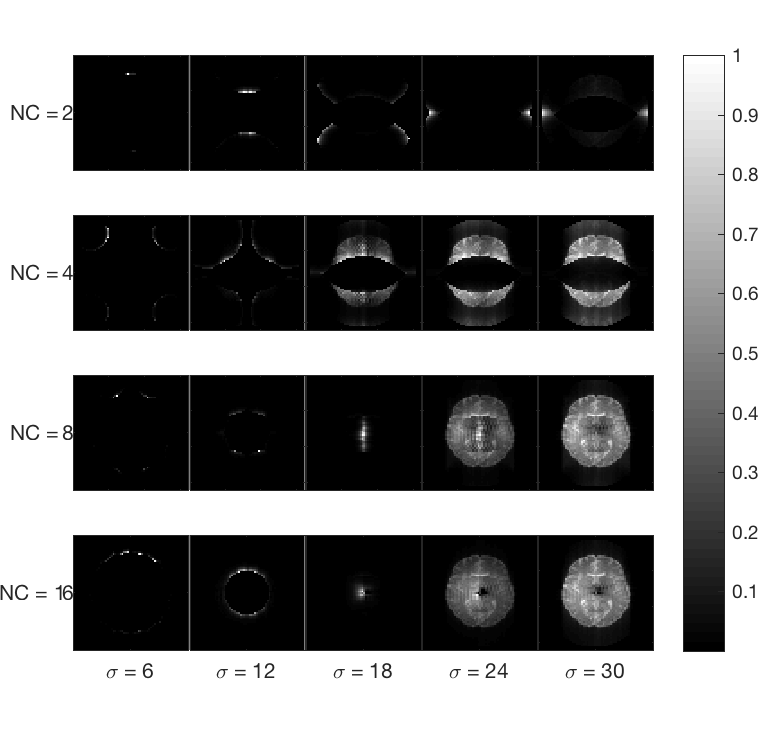
\includegraphics[width=1\textwidth,keepaspectratio]{R3brainsb}
    \caption{SENSE reconstructions for acceleration factor $R = 3$, for increasing numbers of coils on the y-axis and with varying standard deviations of their associated sensitivity profiles on the x-axis}
    \label{fig:R3brains}
\end{figure}

\begin{figure}[H]
    \centering
    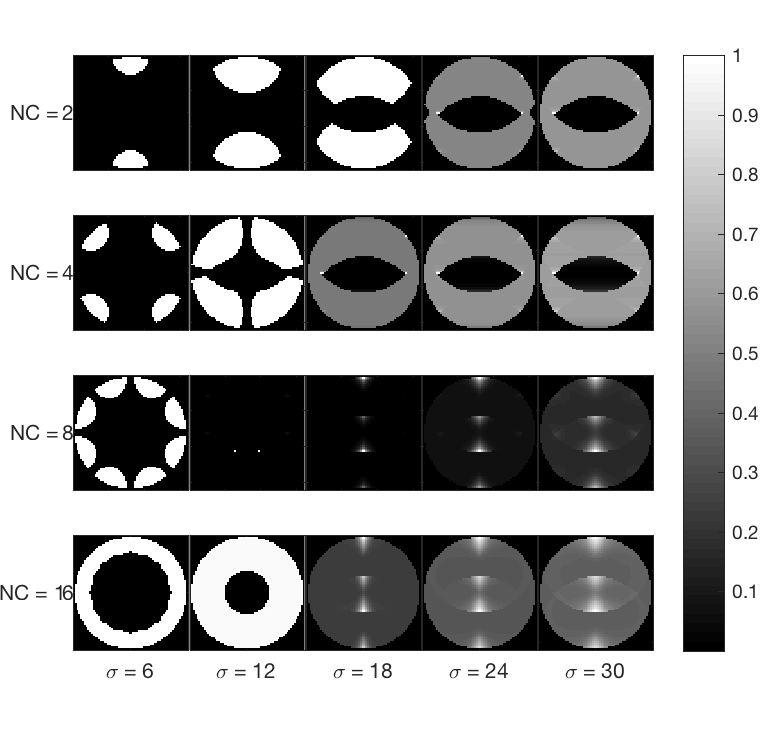
\includegraphics[width=1\textwidth,keepaspectratio]{R3gfactb}
    \caption{g-factor maps for acceleration factor $R = 3$, for increasing numbers of coils on the y-axis and with varying standard deviations of their associated sensitivity profiles on the x-axis}
    \label{fig:R3gfact}
\end{figure}

%% R4
\begin{figure}[H]
    \centering
    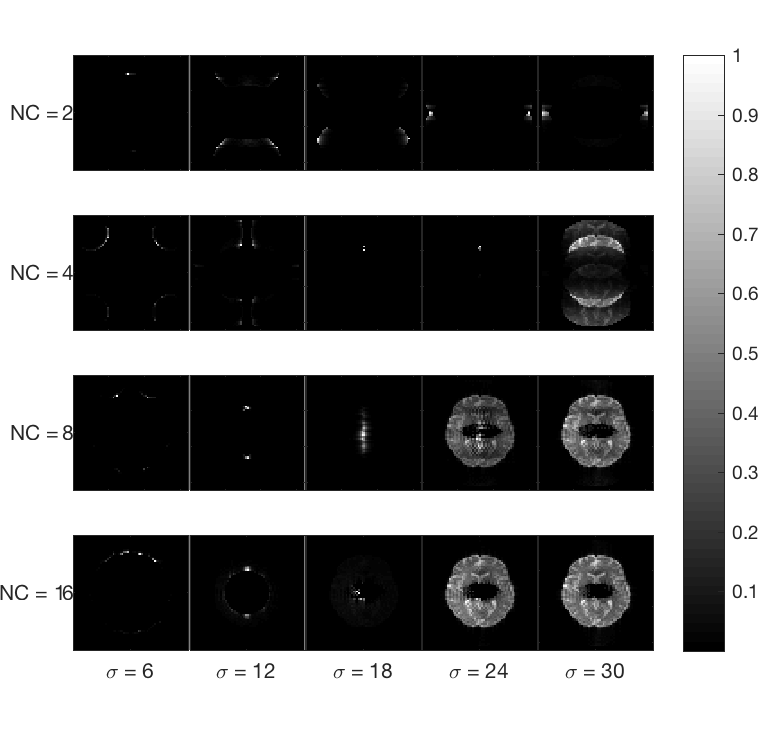
\includegraphics[width=1\textwidth,keepaspectratio]{R4brainsb}
    \caption{SENSE reconstructions for acceleration factor $R = 4$, for increasing numbers of coils on the y-axis and with varying standard deviations of their associated sensitivity profiles on the x-axis}
    \label{fig:R4brains}
\end{figure}

\begin{figure}[H]
    \centering
    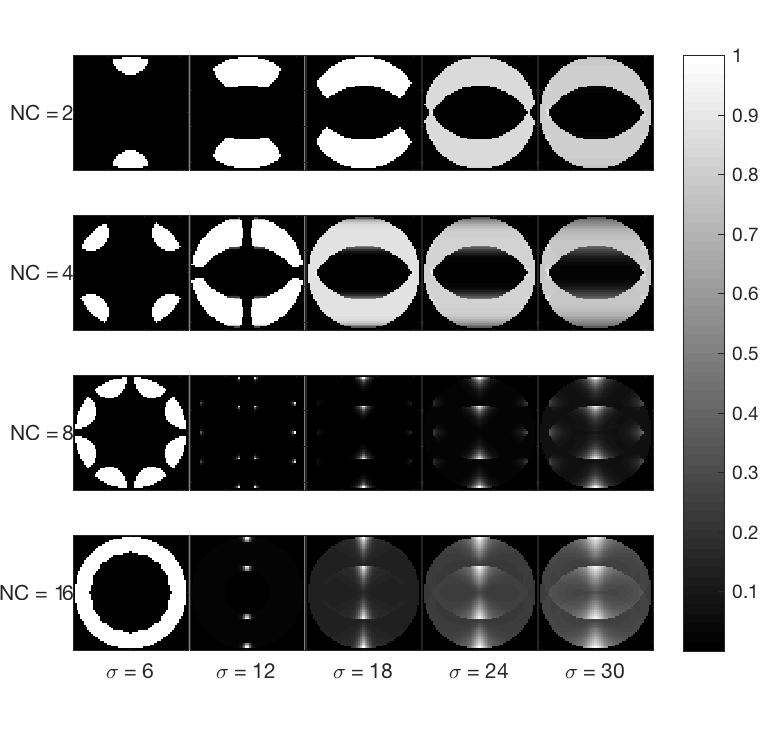
\includegraphics[width=1\textwidth,keepaspectratio]{R4gfactb}
    \caption{g-factor maps for acceleration factor $R = 4$, for increasing numbers of coils on the y-axis and with varying standard deviations of their associated sensitivity profiles on the x-axis}
    \label{fig:R4gfact}
\end{figure}

%%%%%% SSD PLOT
\begin{figure}[H]
    \centering
    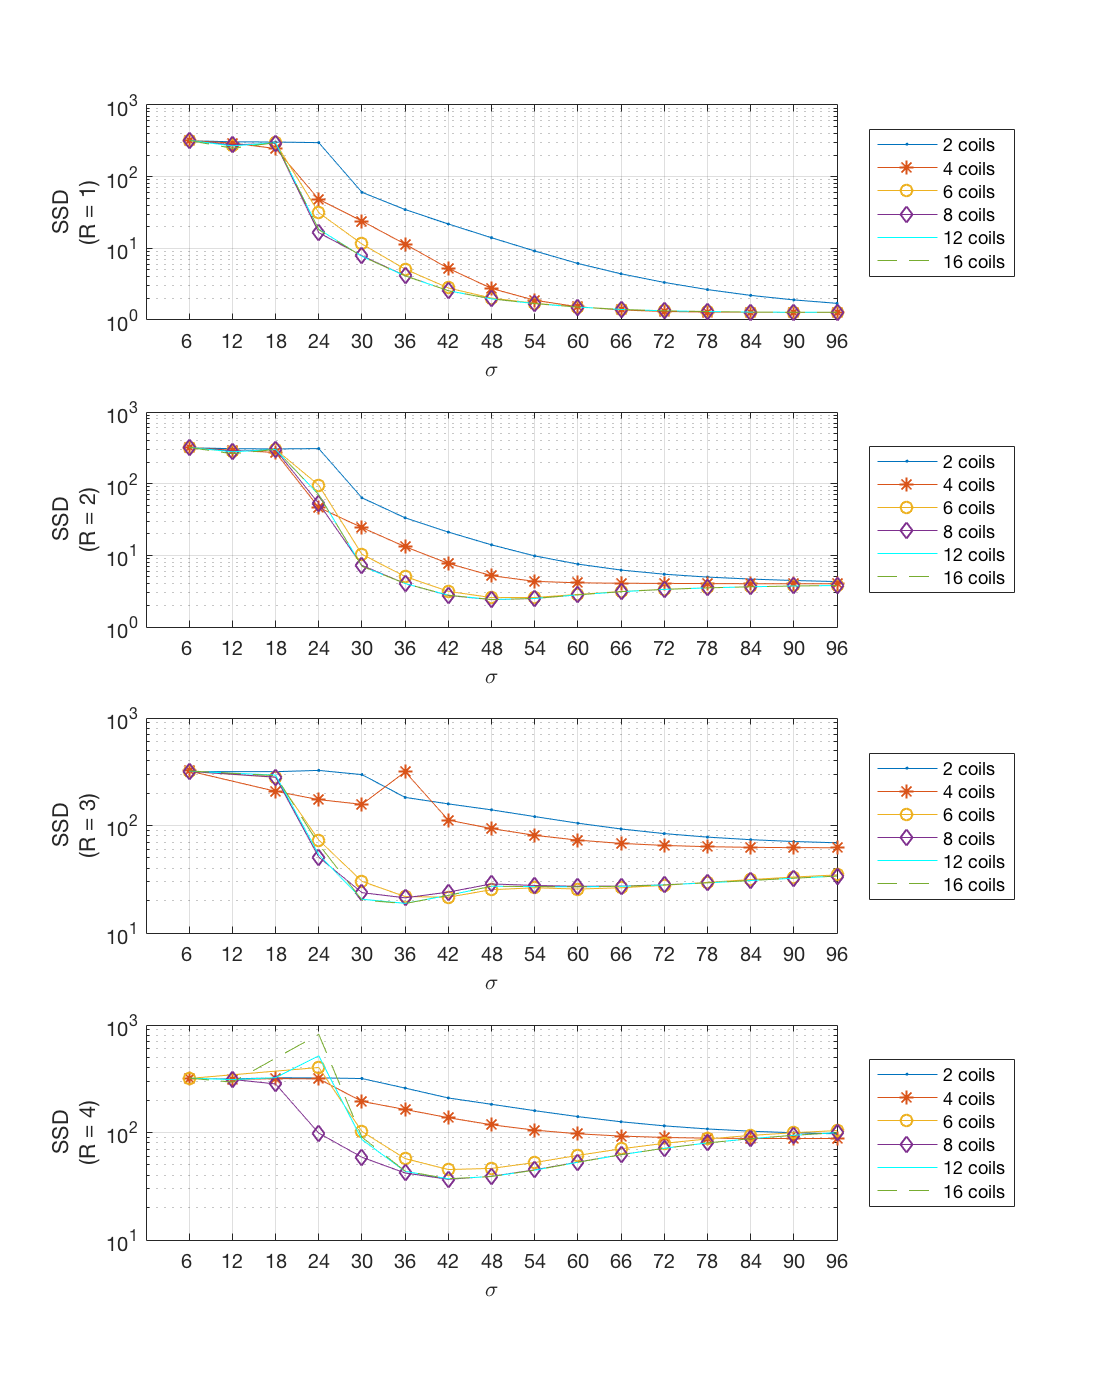
\includegraphics[width=1\textwidth,keepaspectratio]{2SSD}
    \caption{SSD for all acceleration factors, for all coil combinations and for all deviations of their associated sensitivity profiles}
    \label{fig:2SSD}
\end{figure}

\begin{figure}[H]
    \centering
    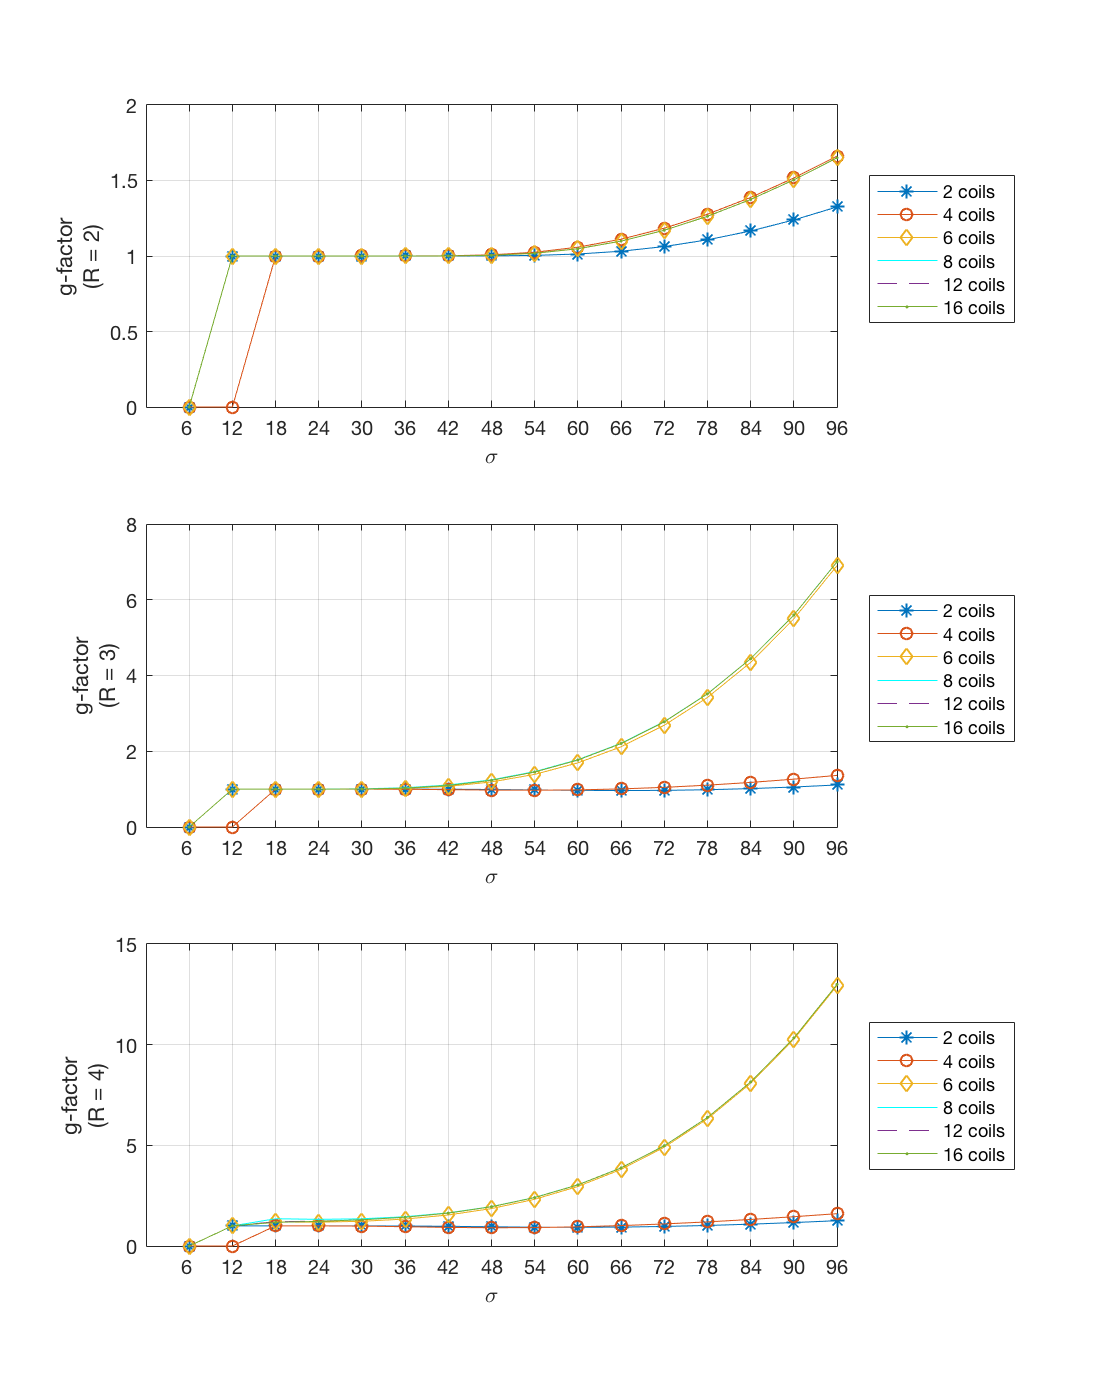
\includegraphics[width=1\textwidth,keepaspectratio]{2gfactor}
    \caption{ROI "g-factor" values for increasing acceleration factors, coil numbers and standard deviations of the associated sensitivity maps}
    \label{fig:2gfactor}
\end{figure} 

\begin{figure}[H]
    \centering
    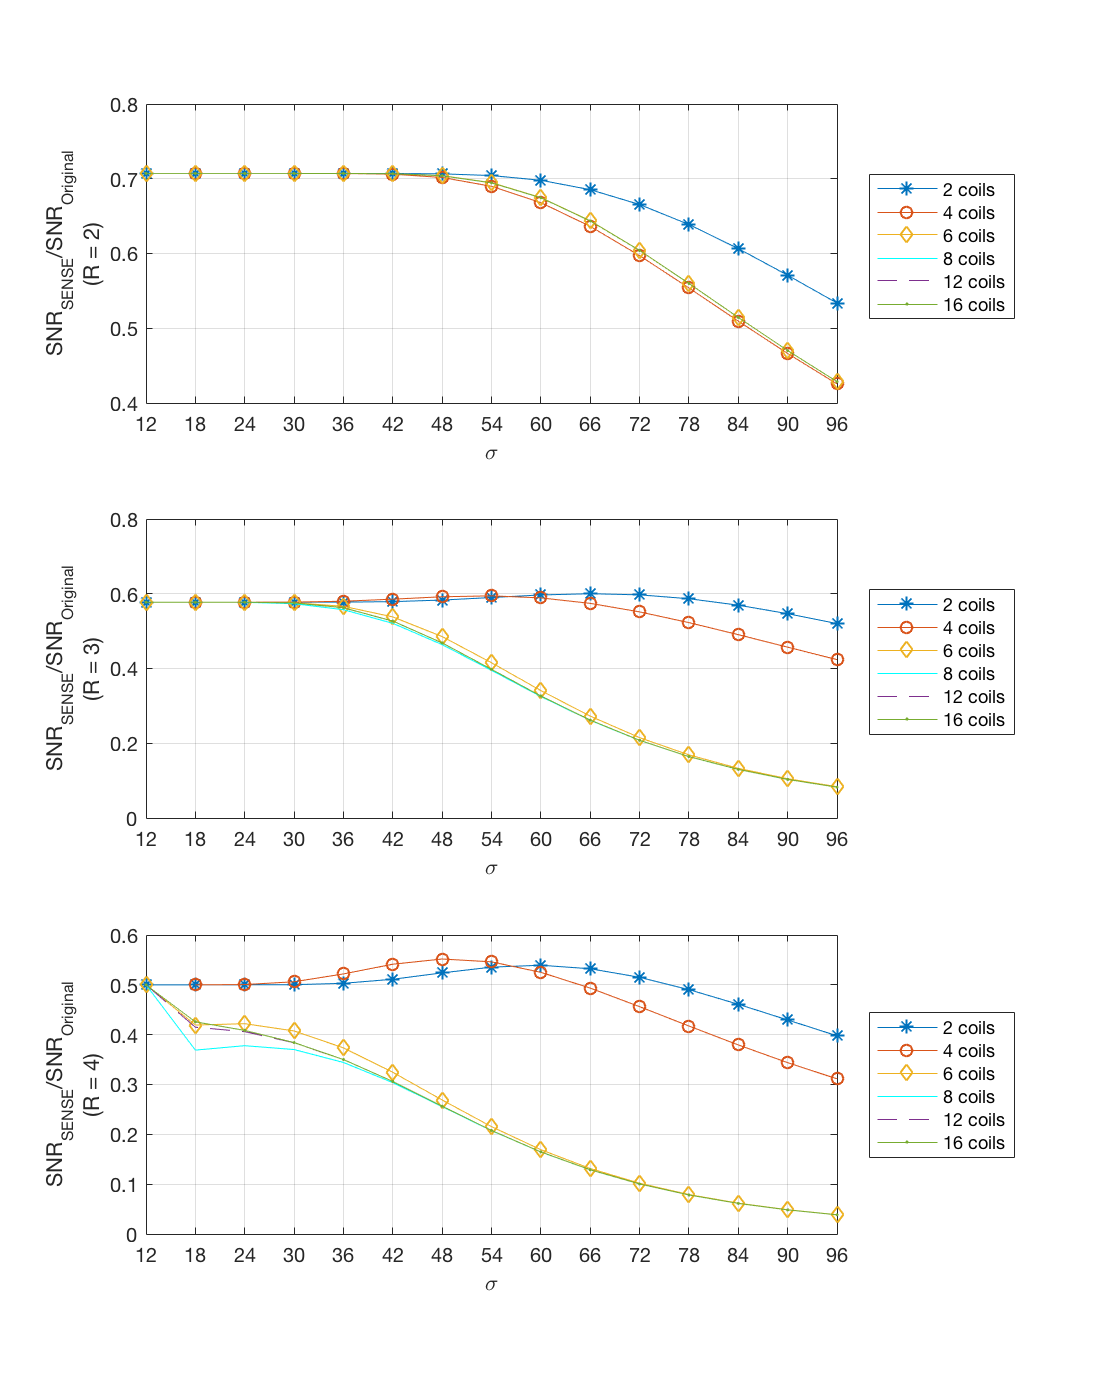
\includegraphics[width=1\textwidth,keepaspectratio]{2SNRsense}
    \caption{The relative decrease in SNR for increasing acceleration factors, coil numbers and standard deviations of the associated sensitivity maps}
    \label{fig:2SNRsense}
\end{figure}


%%%%%%%%%%%%%%%
\section{Influence of noise on SENSE reconstructions}
We have seen so far how SENSE reconstruction is performed with accurate sensitivity maps. However, in a clinical setting, the sensitivity profiles are never perfect and have inherent noise. Moreover, the maps used for reconstruction are acquired during a pre-scan and any patient movement will lead to inaccurate sensitivity profiles and low quality reconstructions. 

Therefore, this section is concerned with reconstructions performed with different levels of noise added to the coil sensitivity maps. The aim of this experiment is to investigate how the quality of reconstruction under these circumstances is affected. One of the major drawbacks of SENSE is not having accurate sensitivity profiles for reconstruction. Errors in these maps will translate into poor reconstructions or even residual aliasing \cite{Deshmane2012}. 

\subsection{Design}
As before, in this experiment we will consider four acceleration factors, different numbers of coils in the array and increasing standard deviations of their associated sensitivity maps. POSSUM simulations were performed with noise-free sensitivity profiles, leaving the white noise addition to the reconstruction step.

The noise was generated from a zero-centered normal distribution $\mathcal{N}(0, \sigma^2)$. We varied the standard deviation of the noise to test the robustness of the reconstruction algorithm and performed simulations for increasing acceleration factors and different numbers of coils. The results can be seen in the following subsection.

\subsection{Results}
As stated before, this experiment is focused on the quality of reconstruction for different levels of noise added to the sensitivity maps. The standard deviation of the normal distribution used to model the noise was ranged from 0 to 2, where for $\sigma = 0$ means no amount of noise is added. More specifically, the values used are: $\sigma_n = \{ 0, 0.001, 0.005, 0.01, 0.05, 0.1, 0.5, 1, 1.5, 2\}$.

The simulations were run for all combinations of coils and for all acceleration factors. The standard deviation of the coil sensitivity profile was set to $\sigma = 48$. The reason behind this decision is that, as can be seen in Figure~\ref{fig:2SSD}, it is one of the points of minimum SSD between accelerated reconstructions and the original image. From this point upward the quality of reconstruction decreases, so it was considered to be a good trade off between all the varying parameters.

The results for SENSE reconstructions are presented in Figures \ref{fig:R1recsnoisej}, \ref{fig:R2recsnoisej}, \ref{fig:R3recsnoisej} and \ref{fig:R4recsnoisej}, whereas the geometry factor maps are presented in Figures \ref{fig:R1gfactnoisej}, \ref{fig:R2gfactnoisej}, \ref{fig:R3gfactnoisej} and \ref{fig:R4gfactnoisej}. Moreover, a sum-of-squared differences was performed between every reconstruction and the original, non-aliased, image. The results are presented in Figure~\ref{fig:ssdnoise}, where every plot shows a different acceleration factor.

\subsection{Discussion}
In this experiment we varied the standard deviation of the noise added to the sensitivity maps used for reconstruction. We then performed SENSE reconstructions for all considered acceleration factors and combinations of coil arrays.

Undoubtedly, the results show that an increase in the level of noise will affect the subsequent reconstructions. The main reason behind this phenomenon is that SENSE-type algorithms rely on accurate sensitivity maps to recover the underlying signal. This is because the first assumption that is made in image based parallel imaging techniques is that every folded spatial location within the aliased images is a juxtaposition of the individual coil sensitivity weighted signal values. Therefore, when the coil maps are changed, the underlying signal can no longer be accurately recovered. This is, of course, directly related to the amount of change brought to these maps, meaning that when the standard deviation of the noise is small, the sensitivity profiles are not changed significantly and relatively accurate reconstructions can still occur. This is also visible in Figures \ref{fig:R1recsnoisej}, \ref{fig:R2recsnoisej}, \ref{fig:R3recsnoisej} and \ref{fig:R4recsnoisej}, where SENSE reconstructions are shown for $\sigma_n$ values between $0$ and $2$.

In fact, as it is presented in Figure~\ref{fig:ssdnoise}, all parameters which were varied in this experiment contribute to a certain extent to the final reconstructions. First, keeping the acceleration factor and the number of coils fixed, it is visible that an increase in noise will directly affect the reconstruction. Clearly, when the acceleration factor is bigger than the number of coils in the array, reconstructions are no longer reliable. That is because in order to unfold aliased locations, one needs at least as many coils as the folded pixels to contribute with the missing information from skipped phase-encoding lines. Second, when the number of receiver channels is increased, the SSD between reconstructions and the original image decreases. This means that when multiple channels are used, reconstructions are more robust to noise. Finally, increasing the acceleration factor leads to worse reconstructions for lower standard deviations of the noise. 
%Actually, this is one of the biggest drawbacks of SENSE-type reconstructions: the need for correct sensitivity profiles of the coils in order to perform as expected and to accurately unfold the aliased images. 

Admittedly, this experiment only shows how different levels of noise added to the sensitivity maps used for SENSE reconstructions affect the quality of the final images. However, two other cases can be identified. First, MRI images are known to be affected by noise. A different experiment would therefore be constructed around accurate sensitivity maps and noisy MRI data, with different levels of noise considered and reconstructions performed for each. Second, as in reality, every piece of electronic equipment has inherent noise, both sensitivity maps and aliased images would have noise added to them. These two scenarios are left for future work.

%% R1
\begin{figure}[H]
    \centering
    \includegraphics[width=1\textwidth,keepaspectratio]{R1recnoiseb}
    \caption{SENSE reconstructions for acceleration factor $R = 1$, for increasing numbers of coils and for different standard deviations of the noise}
    \label{fig:R1recsnoisej}
\end{figure}

\begin{figure}[H]
    \centering
    \includegraphics[width=1\textwidth,keepaspectratio]{R1gfactnoiseb}
    \caption{g-factor maps for acceleration factor $R = 1$, for increasing numbers of coils and for different standard deviations of the noise}
    \label{fig:R1gfactnoisej}
\end{figure}

%% R2
\begin{figure}[H]
    \centering
    \includegraphics[width=1\textwidth,keepaspectratio]{R2recnoiseb}
    \caption{SENSE reconstructions for acceleration factor $R = 2$, for increasing numbers of coils and for different standard deviations of the noise}
    \label{fig:R2recsnoisej}
\end{figure}

\begin{figure}[H]
    \centering
    \includegraphics[width=1\textwidth,keepaspectratio]{R2gfactnoiseb}
    \caption{g-factor maps for acceleration factor $R = 2$, for increasing numbers of coils and for different standard deviations of the noise}
    \label{fig:R2gfactnoisej}
\end{figure}

%% R3
\begin{figure}[H]
    \centering
    \includegraphics[width=1\textwidth,keepaspectratio]{R3recnoiseb}
    \caption{SENSE reconstructions for acceleration factor $R = 3$, for increasing numbers of coils and for different standard deviations of the noise}
    \label{fig:R3recsnoisej}
\end{figure}

\begin{figure}[H]
    \centering
    \includegraphics[width=1\textwidth,keepaspectratio]{R3gfactnoiseb}
    \caption{g-factor maps for acceleration factor $R = 3$, for increasing numbers of coils and for different standard deviations of the noise}
    \label{fig:R3gfactnoisej}
\end{figure}

%% R4
\begin{figure}[H]
    \centering
    \includegraphics[width=1\textwidth,keepaspectratio]{R4recnoiseb}
    \caption{SENSE reconstructions for acceleration factor $R = 4$, for increasing numbers of coils and for different standard deviations of the noise}
    \label{fig:R4recsnoisej}
\end{figure}

\begin{figure}[H]
    \centering
    \includegraphics[width=1\textwidth,keepaspectratio]{R4gfactnoiseb}
    \caption{g-factor maps for acceleration factor $R = 4$, for increasing numbers of coils and for different standard deviations of the noise}
    \label{fig:R4gfactnoisej}
\end{figure}

%% SSD
\begin{figure}[H]
    \centering
    \includegraphics[width=1\textwidth,keepaspectratio]{ssdnoise}
    \caption{SSD between reconstructions and original non-aliased image, for all acceleration factors, for all coil combinations and for all standard deviations of the noise}
    \label{fig:ssdnoise}
\end{figure}

%%%%%%%%%%%%%%%%%%%%%%%%%%%%%%%%
% \section{Motion effects on Parallel Imaging reconstructions}
% Parallel imaging techniques are widely used clinically as they reduce scan time without losing spatial resolution of the final images. This improves patient comfort, is more cost effective and can also reduce motion artifacts. As most MR acquisitions are prone to motion-related artifacts, this section is concerned with investigating the effects of motion when parallel imaging is performed.

% For this, SENSE reconstructions will be performed for different acceleration factors $R = \{1, 2, 3, 4\}$, for all presented channel array combinations (see Figure~\ref{fig:brainsAndCoilsDistrib}) and for all 16 coverage ranges (see Figure~\ref{fig:1coildifsigmas}). Reconstructions will be compared with the original, non-aliased image.

% \subsection{Design}
% In order to simulate motion, POSSUM requires as input a motion sequence file. This file must contain the following parameters, in the specified order: time (in seconds), $T_x$, $T_y$, $T_z$ (translations along all 3 axis, in meters) and $R_x$, $R_y$, $R_z$ (rotations about the specified axis, in radians). For this experiment, a motion file was designed such that the object rotates about the z-axis (yaw) starting from a certain time point. This design choice was made in order to see that parallel imaging techniques, as they require less time to acquire the data, will no longer be affected by the object's movements. The motion file is plotted in Figure~\ref{fig:motioniri}.

% \begin{figure}[H]
%     \centering
%     \includegraphics[width=1\textwidth,keepaspectratio]{motioniri}
%     \caption{Motion sequence file}
%     \label{fig:motioniri}
% \end{figure}

% When simulations are performed with acceleration factor $R = 1$, the 64 phase-encoding lines of k-space are acquired in 50ms, while the middle k-space is being acquired after the first 30ms ($TE_{eff} = 0.03s$). However, increasing acceleration factors will shorten the echo train making it less likely for the acquisition to be affected by motion. In this experiment we investigate whether this scenario holds true.

% As can be seen in Figure~\ref{fig:motioniri}, the motion sequence was designed to start after $TE_{eff}$, but before the end of the $R = 1$ slice acquisition. As the object (the brain, in our case) will rotate only during the latter part of the acquisition, blurring will be seen in the final image. As more than half of k-space lines were acquired when no motion was involved, the reason behind the blurring comes from the faulty lines acquired during motion. Figure~\ref{fig:motionvsnomotion} shows the motion corrupted image, as well as the no motion case and the absolute difference between the two.

% \begin{figure}[H]
%     \centering
%     \includegraphics[width=1\textwidth,keepaspectratio]{motionvsnomotion}
%     \caption{The two cases are presented: the no motion case can be seen in the left hand side of the figure, the motion corrupted case is found in the middle image, and the absolute difference between the two is presented in the right hand side of the figure. The blurring artifact is visible in the middle image.}
%     \label{fig:motionvsnomotion}
% \end{figure}

% For this experiment, simulations were run for all 4 acceleration factors, all 6 coil combinations and all 16 sensitivity maps. A region of interest was chosen on the final images and a sum-of-squared differences was performed between all reconstructions and the no motion case. These results were compared with the SSD between the motion case and no motion when parallel imaging was not used. The reason for this was to see that with higher acceleration factors, the reconstructions will be less prone to motion and therefore more close to the no motion case.

% \subsection{Results}
% Motion during MRI scans causes the excited spins to change position between phase-encoding gradients and signal reading. As a result, motion artifacts appear in the final images mainly in the phase-encoding direction. For this reason, the region of interest chosen in this experiment spans across the y-direction more so than across the x-direction. Figure \ref{fig:brainroi} shows the ROI in both the motion and no motion cases.

% \begin{figure}[H]
%     \centering
%     \includegraphics[width=1\textwidth,keepaspectratio]{brainroi}
%     \caption{The chosen ROI shown for both motion and no motion cases}
%     \label{fig:brainroi}
% \end{figure}

% As stated before, simulations were run for the motion case for all acceleration factors, all coil combinations and all sensitivity maps. Figure \ref{fig:resultsexp4} shows the results of this experiment. Each plot represents a different acceleration factor $R$, while the x-axis of these plots represents the standard deviations of the sensitivity profiles, in increasing order. The y-axis is in logarithmic scale and represents the sum-of-squared differences between the reconstructions and the no motion original image. Moreover, the green line shown in each plot represents the SSD between the motion and no motion cases presented in Figure~\ref{fig:motionvsnomotion}.

% The best results can be seen in the second plot, where acceleration factor $R = 2$. The SENSE reconstruction for the 2-coil array, for $\sigma = 72$ is shown in Figure~\ref{fig:bestrec}. The other combinations of parameters show promising results as well, although, when $\sigma < 72$, the reconstructions do not perform well enough. Moreover, the simulations performed with $R > 2$ do not perform as well due to ill-conditioned reconstructions. These drawbacks of the method were presented in Section \ref{exp2}. 

% \begin{figure}[H]
%     \centering
%     \includegraphics[width=1\textwidth,keepaspectratio]{resultsexp4all}
%     \caption{SSD between reconstructions and original non-aliased image, for all acceleration factors, for all coil combinations and for all standard deviations of the sensitivity profiles. In green, the SSD between the original non-aliased image and the original motion simulated image is shown. All values shown are for a chosen ROI as presented in Figure \ref{fig:brainroi}}
%     \label{fig:resultsexp4}
% \end{figure}

% \begin{figure}[H]
%     \centering
%     \includegraphics[width=1\textwidth,keepaspectratio]{bestrec}
%     \caption{The no motion and motion cases are shown in the left hand side and the right hand side of the image, while SENSE reconstruction for $R = 2$, $\sigma = 72$ and a 2 coil channel array is shown in the middle}
%     \label{fig:bestrec}
% \end{figure}

% \subsection{Discussion}
% In this experiment, a motion sequence was defined and used as input to our simulations in order to investigate the effect of object movement when parallel imaging is performed for various acceleration factors. Figure~\ref{fig:motionvsnomotion} shows the SSD between all SENSE reconstructions and the original non-aliased image. 

% First, it is visible from the plot that when no acceleration is in place, meaning $R = 1$, the reconstruction resembles the motion case as presented in Figure~\ref{fig:motionvsnomotion}. For the first 9 standard deviations of the sensitivity maps, the reconstruction is poor as the coil profile's coverage is not large enough to encompass the necessary field-of-view. For the last 7 sensitivity profiles, reconstruction can be performed. As all SENSE reconstructions are basically the original, motion simulated image, the SSD between the chose ROIs will be the same as the SSD between the two original cases, when parallel imaging is not involved.

% Second, when acceleration factor 2 is used, the echo train becomes small enough that it does not encompass the motion anymore. That is clearly visible from the second plot where all reconstructions, for the sensitive enough coil profiles, perform better in terms of SSD than the original motion simulated image. 

% Finally, when higher acceleration factors are used, as was presented in Section \ref{exp2}, the quality of reconstruction drops significantly. Moreover, when $R > 2$ and an array with 2 channels is used, reconstructions cannot be performed as the number of juxtaposed signals in the aliased images is greater than the available coil information. Thus, the results show an outlier which just happened to be closer to the original non-aliased image, making the SSD drop significantly.

% All in all, this has been a proof of concept experiment. It is evident from the results shown that motion is a highly complicated aspect of MRI simulation that requires more cases than the one presented. First of all, motion was present for less than half of the k-space acquisition time. As movement can happen throughout the read-out period, an experiment involving motion throughout the whole signal acquisition should be considered. Second, reconstructions for $R > 2$ did not perform well to begin with, making this experiment less likely to show major improvements for such cases. Next, the conclusions and future work will be presented.


















\chapter{Conclusions and Future Work}
\label{chapterconclusions}

%%%%%%%%%%%%%%%%%%%%%%
\section{Overview}
The main aim of this thesis was to enhance the functionality of the already existing MRI simulator POSSUM with parallel imaging capabilities. In particular, the entire pipeline was considered, from coil sensitivity maps generation to parallel imaging reconstruction. In addition, an image-based reconstruction algorithm was considered and tested with the newly implemented pipeline for various combinations of parameters. Towards the achievement of these goals, the next steps were taken:

\begin{itemize}
    \item Multi-coil acquisition capabilities were added to POSSUM. As the first step towards simulating partially parallel magnetic resonance imaging is to model acquisition with multiple receiver coils, different sensitivity profiles for non-homogeneous surface coils were generated and used in all the simulations presented in this thesis.
    
    \item The parallel imaging pipeline was simulated with the enhanced version of POSSUM. For this, the previously generated sensitivity profiles were used in a variety of scenarios. First, the number of coils in the array was varied. Simulations were done with arrays of 2, 4, 6, 8, 12 and 16 channels. Second, different spatial variations of the sensitivity profiles was considered in order to encompass both too low coil sensitivity and too high sensitivity as the range extremes. 
    
    \item The performance of a SENSE-type reconstruction algorithm was evaluated. For this, the quality of the proposed reconstruction algorithm was tested under increasing acceleration factors. Moreover, noise was added to the sensitivity maps of the coils and SENSE reconstructions were again performed for all combinations of the parameters described above in order to evaluate its robustness to noise.
\end{itemize}

%%%%%%%%%%%%%%%%%%%%%%
\section{Conclusions}
Partially parallel magnetic resonance imaging techniques were born from the need of reducing MRI scan time. Indeed, other approaches have been made towards this goal, but all of them were focused on developing faster sequences which eventually reached a technical plateau. The advantage of pMRI is that it works in conjunction with already established MRI sequences. In fact, these techniques are popular enough that they are part of the standard imaging pipeline of many clinically available scanners. However, as with any other MRI technique, these are also prone to a handful of problems which need to be investigated in a controlled and reliable manner.

That being said, the only way of accurately assessing the reconstruction schemes which are used in pMRI is to simulate the parallel imaging acquisition pipeline. As a result, the main aim of this thesis was to enhance an already existing MRI simulator called POSSUM with parallel imaging capabilities and to test a popular image based reconstruction algorithm called SENSE under various combinations of parameters. In doing so, the following points can be concluded:

\begin{itemize}
    \item The newly enhanced POSSUM can now simulate the parallel imaging pipeline. When this option is considered, a collection of coil sensitivity maps, together with the acceleration factor desired, must be provided as input to the simulator. In doing so, POSSUM will generate non-aliased (when $R = 1$) or aliased (when $R > 1$) images for each individual coil. 

    \item Having generated this dataset, an image based parallel imaging reconstruction algorithm was then tested. As SENSE-type algorithms are known to be affected by the reduction of phase-encoding lines and by the accuracy of the sensitivity maps, both these scenarios were investigated:
    
    \begin{itemize}
        \item First, different acceleration factors were considered and tested for various combinations of coils and sensitivity profiles. It was found that a good balance between the coil geometry and the acceleration factor needs to be found as both parameters are generally extremely important for accurate reconstructions. In fact, there are two types of imaging artifacts which are known to affect SENSE reconstructions: residual aliasing and noise enhancement. Both were found in our simulations as a consequence of the high dependency between the considered parameters.
        
        \item Second, as the quality of SENSE reconstructions is known to be directly affected by the accuracy of the coil sensitivity profiles, an experiment was devised in which different levels of noise were added to the maps used for reconstructions. As expected, it was found that all of the above described parameters are important. More specifically, increasing the acceleration factor will lead to poorer reconstructions for lower levels of noise, while increasing the number of channels in the array will lead to more accurate reconstructions and therefore a higher robustness to noise. 
        
    \end{itemize}

\end{itemize}

All in all, the main aim of this thesis was achieved. This was the first step towards a full integration within POSSUM of the parallel imaging pipeline. In addition, we showed that a popular image based pMRI reconstruction algorithm can be tested with the simulated data sets under various scenarios. That being said, this current work leads to promising avenues for future research.

%%%%%%%%%%%%%%%%%%%%%%
\section{Future Work}
The research done in this thesis is not without limitations. That being said, this section is concerned with looking at future improvements and directions.

The first direction which will be taken as a consequence of this work is to improve upon the literature review chapter. The main aim here is to turn this early work into a \textit{review paper of MRI simulators}.

In addition, the current state of this work will be extended. The first step towards this goal is to \textit{integrate the parallel imaging pipeline within POSSUM}, together with the reconstruction algorithm. Moreover, a tutorial for how to seamlessly interact with the newly enhanced software will be created for anyone to easily use the new capabilities.

Next, \textit{coil geometry} should be investigated. In parallel imaging techniques, great thought is put into developing the phased-array coil used for signal acquisition. One of its most important aspects is the physical positions of the coils with respect to the object being imaged. More specifically, for accurate reconstructions, the array of channels must be positioned in such a way that their inherent sensitivity profiles are spatially varying in the direction of acceleration. As a lot of research is done in this area, a more informed approach to the creation of the coil arrays could improve the subsequent reconstructions.

% On top of that, \textit{coil sensitivity profiles} are of utmost importance for . In this thesis, the coil sensitivity profiles were generated to spatially vary isotropically starting at the coil centre. A more realistic way of generating sensitivity maps is described by Pruessmann et al \cite{Pruessmann1999} in their SENSE paper. The authors state that sensitivity map determination can be done by acquiring a collection of full FOV images during a pre-scan for each individual coil and dividing each one of them to the "sum-of-squares" of the set. However, this approach leads to noisy maps which have to be smoothed out with a 2D polynomial fit in each pixel location. Nevertheless, it is an avenue worth exploring.

Moreover, \textit{K-space reconstruction algorithms} should be added. In this thesis the focus was on image based reconstructions. A second type of reconstruction algorithms, which are also used clinically, are called k-space reconstruction algorithms. These techniques have a different approach on determining the missing phase encoding lines as they work directly with the undersampled k-space. Moreover, they require a special pre-scan which collects the middle k-space for each coil without acceleration and uses that information to reconstruct the missing data. A comparison between the 2 types of reconstructions could therefore be evaluated.

Also, as a major source of imaging artifacts is patient movement, \textit{simulating motion} would be of great importance. Motion can be a determining factor when it comes to image quality in magnetic resonance imaging. For this reason, pMRI accelerated sequences are used to acquire signal in between heart beats or respiration. However, motion can still affect the quality of reconstruction especially during readout as different spatial locations within the object will be weighted differently by the sensitivity maps of the channels. Simulating motion would be challenging, but it is an avenue worth exploring.

As a long term goal, given the fact that the main aim of my PhD project is to develop novel MRI biomarkers to measure progression in neurodegenerative diseases, such as Parkinson’s Disease (PD), based on DW-MRI data, the current work will be extended to incorporate diffusion. This could allow for a more accurate representation of the underlying brain microstructure.

% Parkinson’s Disease is a common progressive neurodegenerative disease that manifests clinically with symptoms including tremors and/or imprecise movements. The disease is known to attack substantia nigra, a gray matter structure lying deep inside the brain. Advanced DW-MRI techniques, such as NODDI, have the potential to help us detect the earliest signs of the disorder in terms of subtle changes to tissue microarchitecture, long before the onset of clinical symptoms. This may open an earlier therapeutic window to develop effective preventative treatments.

% However, DW-MRI datasets suffer from a range of imaging artifacts and challenges that are more acute in patients with PD. Common imaging artifacts include severe geometric distortions due to magnetic susceptibility differences at the air-tissue interfaces and eddy currents induced by diffusion sensitising gradients. In patients with PD, these are compounded by patient motion. Furthermore, substantia nigra, the key region of interest, is plagued with poor signal-to-noise ratio. Simulation provides a controlled way of studying these, understanding how they impact the quantification of tissue microstructure, and ultimately develop methods to mitigate their impact.

\addcontentsline{toc}{chapter}{Appendices}

% The \appendix command resets the chapter counter, and changes the chapter numbering scheme to capital letters.
%\chapter{Appendices}
%%%%%%%%%%%%%%%%%%%%%%%%%%%%%%%%%%%%%%%%%%%%%%%%%%%%%%%%%%%%%%%
%% APPENDIX 1
\appendix
\chapter{Coil sensitivity profiles by number of channels}
\label{appendixlabel1}

\begin{figure}[H]
    \centering
    \includegraphics[width=.8\textwidth,keepaspectratio]{2coilsdifsigmas}
    \caption{Coil sensitivity maps of the 2-channel arrangement}
\end{figure}

\begin{figure}[H]
    \centering
    \includegraphics[width=.8\textwidth,keepaspectratio]{4coilsdifsigmas}
    \caption{Coil sensitivity maps of the 4-channel arrangement}
\end{figure}

\begin{figure}[H]
    \centering
    \includegraphics[width=.8\textwidth,keepaspectratio]{6coilsdifsigmas}
    \caption{Coil sensitivity maps of the 6-channel arrangement}
\end{figure}

\begin{figure}[H]
    \centering
    \includegraphics[width=.8\textwidth,keepaspectratio]{8coilsdifsigmas}
    \caption{Coil sensitivity maps of the 8-channel arrangement}
\end{figure}

\begin{figure}[H]
    \centering
    \includegraphics[width=.8\textwidth,keepaspectratio]{12coilsdifsigmas}
    \caption{Coil sensitivity maps of the 12-channel arrangement}
\end{figure}

\begin{figure}[H]
    \centering
    \includegraphics[width=.8\textwidth,keepaspectratio]{16coilsdifsigmas}
    \caption{Coil sensitivity maps of the 16-channel arrangement}
\end{figure}

%%%%%%%%%%%%%%%%%%%%%%%%%%%%%%%%%%%%%%%%%%%%%%%%%%%%%%%%%%%%%%%
%% APPENDIX 2
% \chapter{"g-factor" maps for different acceleration factors}
% \label{appendixlabel2}

% %% R = 1
% \begin{figure}[H]
%     \centering
%     \includegraphics[angle=90,width=.6\textwidth,keepaspectratio]{R1gfactsgm916_new}
%     \caption{g-factor maps for acceleration factor $R = 1$, for increasing numbers of coils on the y-axis and with varying standard deviations of their associated sensitivity profiles on the x-axis}
% \end{figure}

% \begin{figure}[H]
%     \centering
%     \includegraphics[angle=90,width=.6\textwidth,keepaspectratio]{R1gfactsgm18_new}
%     \caption{g-factor maps for acceleration factor $R = 1$, for increasing numbers of coils on the y-axis and with varying standard deviations of their associated sensitivity profiles on the x-axis}
% \end{figure}

% %% R = 2
% \begin{figure}[H]
%     \centering
%     \includegraphics[angle=90,width=.6\textwidth,keepaspectratio]{R2gfactsgm18_new}
%     \caption{g-factor maps for acceleration factor $R = 2$, for increasing numbers of coils on the y-axis and with varying standard deviations of their associated sensitivity profiles on the x-axis}
% \end{figure}

% \begin{figure}[H]
%     \centering
%     \includegraphics[angle=90,width=.6\textwidth,keepaspectratio]{R2gfactsgm916_new}
%     \caption{g-factor maps for acceleration factor $R = 2$, for increasing numbers of coils on the y-axis and with varying standard deviations of their associated sensitivity profiles on the x-axis}
% \end{figure}

% %% R = 3
% \begin{figure}[H]
%     \centering
%     \includegraphics[angle=90,width=.6\textwidth,keepaspectratio]{R3gfactsgm18_new}
%     \caption{g-factor maps for acceleration factor $R = 3$, for increasing numbers of coils on the y-axis and with varying standard deviations of their associated sensitivity profiles on the x-axis}
% \end{figure}

% \begin{figure}[H]
%     \centering
%     \includegraphics[angle=90,width=.6\textwidth,keepaspectratio]{R3gfactsgm916_new}
%     \caption{g-factor maps for acceleration factor $R = 3$, for increasing numbers of coils on the y-axis and with varying standard deviations of their associated sensitivity profiles on the x-axis}
% \end{figure}

% %% R = 4
% \begin{figure}[H]
%     \centering
%     \includegraphics[angle=90,width=.6\textwidth,keepaspectratio]{R4gfactsgm18_new}
%     \caption{g-factor maps for acceleration factor $R = 4$, for increasing numbers of coils on the y-axis and with varying standard deviations of their associated sensitivity profiles on the x-axis}
% \end{figure}

% \begin{figure}[H]
%     \centering
%     \includegraphics[angle=90,width=.6\textwidth,keepaspectratio]{R4gfactsgm916_new}
%     \caption{g-factor maps for acceleration factor $R = 4$, for increasing numbers of coils on the y-axis and with varying standard deviations of their associated sensitivity profiles on the x-axis}
% \end{figure}


% \chapter{Colophon}
% \label{appendixlabel3}
% \textit{This is a description of the tools you used to make your thesis. It helps people make future documents, reminds you, and looks good.}

% \textit{(example)} This document was set in the Times Roman typeface using \LaTeX\ and Bib\TeX , composed with a text editor. 
 % description of document, e.g. type faces, TeX used, TeXmaker, packages and things used for figures. Like a computational details section.
% e.g. http://tex.stackexchange.com/questions/63468/what-is-best-way-to-mention-that-a-document-has-been-typeset-with-tex#63503

% Side note:
%http://tex.stackexchange.com/questions/1319/showcase-of-beautiful-typography-done-in-tex-friends 
% You could separate these out into different files if you have
%  particularly large appendices.

% This line manually adds the Bibliography to the table of contents.
% The fact that \include is the last thing before this ensures that it
% is on a clear page, and adding it like this means that it doesn't
% get a chapter or appendix number.
\addcontentsline{toc}{chapter}{Bibliography}

% Actually generates your bibliography.
\bibliography{example}

% All done. \o/
\end{document}
